\documentclass[a4paper, twoside, notitlepage, 10pt]{report}

% admin
\title{MscThesisVenderbosch}
\author{Marijn Venderbosch}
\date{\normalsize \textsf{\today}}

% essentials
\usepackage{type1cm}%arbitrary font size
\usepackage[english]{babel}
\usepackage[top = 1in, left = 1.1in, bottom = 1in, right = 1in]{geometry}
\usepackage{graphicx}
\usepackage{mathtools}
\usepackage{float}
\usepackage{amsmath}
\usepackage{amssymb}
\usepackage[colorlinks = true, linkcolor = Blue2, citecolor = SpringGreen4]{hyperref}%
\usepackage{subcaption}
\usepackage{url}
\usepackage[x11names]{xcolor}
\usepackage{cleveref}
\usepackage{subfiles}
\usepackage[toc,page]{appendix}
\usepackage{tabularx}
\usepackage{array}
\usepackage{setspace}

% braket notation
\DeclarePairedDelimiter\bra{\langle}{\rvert}
\DeclarePairedDelimiter\ket{\lvert}{\rangle}
\DeclarePairedDelimiterX\braket[2]{\langle}{\rangle}{#1 \delimsize\vert #2}

% unit vector
\usepackage{bm}

% enumerate
\usepackage[]{enumitem}
\setlist[enumerate]{itemsep = 2pt, topsep = 4pt}

% appearance
\usepackage[labelfont = {bf, sf}, width=\textwidth]{caption}
\captionsetup{font = {stretch = 1}, figurename = Fig., tablename = Tab.}
\usepackage[bf, sf]{titlesec}
\usepackage{microtype}
\renewcommand{\figurename}{Fig.}
\setstretch{1.09}
\usepackage{blindtext, color}
\setlength{\parskip}{0pt}

% itemize spacing
\setlength{\itemsep}{0pt}

% font
\usepackage[T1]{fontenc}
\usepackage[scaled=1.04]{XCharter}%serif
\usepackage[scaled=0.95]{helvet} % sans serif
\usepackage[]{newtxmath} % math font, options in []. Leave.
\usepackage[scaled=0.9]{DejaVuSansMono} % mono

% page header
\usepackage{fancyhdr}
\setlength{\headheight}{14pt}
\pagestyle{fancy}
\addtolength{\linewidth}{\marginparsep}
\addtolength{\linewidth}{\marginparwidth}
\renewcommand{\chaptermark}[1]{\markboth{\thechapter\ #1}{}}
\renewcommand{\sectionmark}[1]{\markright{\thesection\ #1}}
\fancyhf{}
\cfoot{\textsf{\thepage}}
\fancyhead[LE]{\textsf{{\rightmark}}}
\fancyhead[RO]{\textsf{{\leftmark}}}
\fancypagestyle{plain}{%
	\fancyhead{} % get rid of headers
	\renewcommand{\headrulewidth}{0pt} % and the line
}

% bibliography
\usepackage[backend = bibtex8, , giveninits = true, sorting = none, url = false, isbn = false, maxnames = 3]{biblatex}
\addbibresource{bibliography.bib}

% table of contents
\setcounter{tocdepth}{2}

% acronyms
\usepackage[printonlyused]{acronym}

% section numbering depth
\setcounter{secnumdepth}{3}
% start with roman numbering for frontmatter
\pagenumbering{roman}

% boxes/frames
\usepackage{mdframed}

% metadata pdf
\hypersetup{pdftitle={MScThesisVenderbosch},pdfsubject={Holographic Optical Tweezers for Arrays of Neutral Atoms},pdfauthor={Marijn Venderbosch}}



%DOCUMENT%

\begin{document}


\begin{titlepage}
	\begin{centering}
		\vspace*{3cm}
		
		\textsf{\LARGE \textbf{Holographic Optical Tweezers for Arrays of Single Atoms}}
		
		\vspace{2.5cm}
		
		\textsf{\Large Marijn Leonardus Venderbosch}
		
		\vspace{2cm}
		
		\textsf{\large Supervisors:}
		
		\vspace{0.5cm}
		
		\textsf{\large dr. E.J.D. Vredenbregt\\
			dr. S.J.J.M.F. Kokkelmans
			}
		
		\vfill
		
		\begin{figure}[h]
			\centering
			
\includegraphics[width=6cm]{figures/TUeLogo.png}
		\end{figure}
		
		\textsf{Coherence \& Quantum Technology group}
		
		\vspace{0.4cm}	
		
		\textsf{CQT 2021-03}
		
		\textsf{January 2022}
		
		\vspace{1cm}
		
		
	\end{centering}
\end{titlepage}




\clearpage

\newgeometry{left = 3cm, top = 4cm, right = 3cm, bottom = 4cm}
    \hspace{0pt}
    \vfill
        \renewcommand{\abstractname}{\Large{Abstract}}
        \begin{abstract}
            \thispagestyle{plain}
            \vspace*{0.5cm}
            \normalsize
            %\noindent Recently, quantum computation and simulation have attracted significant interest within the ultra-cold atom community.
We report on the progress towards a neutral-atom based quantum co-processor.
As a first step towards this goal, we constructed a novel apparatus capable of laser-cooling Rb atoms near the Doppler temperature in an optically contacted glass cell (atom number $\sim 10^5, T\sim 200$ $\mu$K). 
Subsequently, the atoms are loaded in an array of optical tweezers made by a spatial light modulator (Meadowlark, $1920 \times 1200$) and a glass-compensated ultra-long working distance microscope objective (Mitutoyo, 0.5 NA) at $\lambdaup = 820$ nm.
We measured the tweezer potentials directly using a 0.85 NA objective, finding a near-diffraction limited waist of $0.79\pm0.05$ $\mu$m (theory: 0.75 $\mu$m) in the radial direction and a Rayleigh range of $6.2 \pm 0.5$ $\mu$m (diffraction theory: 3.0 $\mu$m) in the axial direction.
After aberration correction using the spatial-light modulator we find a corrected Rayleigh range $3.6\pm0.6$ $\mu$m.
The tweezer arrays light distributions showed a typical non-homogeneity of $\sim 10\%$ without active feedback-loop compensation for the hologram producing the spot arrays. 
Atoms in the tweezer array are imaged into a sCMOS camera (Zyla, 5.5 MP) by splitting off the fluorescence using a long pass dichroic mirror.

        \end{abstract}
    \vfill
    \vspace{100pt}
    \clearpage
    
    \hspace{0pt}
    \vfill
        \renewcommand{\abstractname}{\Large{Acknowledgments}}
        \begin{abstract}
            \thispagestyle{plain}
            \vspace*{0.5cm}
            \normalsize
            %\renewcommand{\abstractname}{\textsf{\Large{Acknowledgements}}}

\begin{abstract}
\vspace*{0.5cm}

Er zijn heel veel mensen die me hebben geholpen bij mijn afstudeerproject, daarom zou ik ze graag willen bedanken. Allereerst Edgar, ik heb je begeleiding als zeer prettig ervaren. Niet alleen heb je superveel kennis van zaken, maar als ik weer op een zijspoor zat greeg je me altijd weer op de goede weg met je pragmatische visie. Het was ook prettig dat je vanuit je experimentele ervaring realistische doelen stelde.

Dan Servaas, bedankt voor je nuttige en creatieve ideeën tijdens de wekelijkse bespreekmomenten. Je had altijd een enthousiaste en positieve instelling en stelde spontane dingen voor als een gesprek met Rick van Bijnen.

Vervolgens zou ik de persoon willen bedanken met wie ik de meeste tijd heb doorgebracht. Deon, een groot gedeelte van de voortang met de rubidium tweezer machine zijn te wijden aan jouw aanpassings- en improvisatievermogen. Ook hadden we veel lol in het lab en daarbuiten, bedankt daarvoor. 

Vanaf een iets grotere fysieke afstand, was een ook heel fijn dat ik af en toe even kon sparren met Ivo. Bedankt voor je suggesties en tips over SLM's en optica. Als je naar Eindhoven kwam om een biertje te drinken was het ook altijd gezellig. Ook Alex bedankt voor je enthousiaste en gedetailleerde feedback tijdens de gezamenlijke vergaderingen, en bedankt dat Rik en ik in jullie lab mochten langskomen om te zien wat er bij komt kijken met een ultrakoud strontium experiment. Ook Florian en Robert bedankt voor feedback.

Terug naar Eindhoven zijn veel mensen binnen onze groep die geholpen hebben. Robert en Madhav, bedankt voor inspirerende discussies op theoretisch gebied. Technische hulp was er vanuit Eddy, Harry, Hein en Jeroen, bedankt daarvoor! Ook stonden collega's in het lab altijd klaar om te helpen als ik iets nodig had, bedankt Rik, Luc, Tim, Yang, Sheng en Daniel. Als laatste wil ik de andere groepleden bedanken voor alle koffiepauzes, seminars en borrels. Ik kijk met veel plezier terug op het afgelopen jaar bij CQT! 

\end{abstract}

\newpage
        \end{abstract}
    \vfill
    \vspace{100pt}
\restoregeometry


\tableofcontents
\newpage

% link page containing acronyms
\section*{List of Acronyms}

% add Table of Contents
\addcontentsline{toc}{section}{List of Acronyms}

% surpress fancy header
\thispagestyle{plain}
\pagestyle{fancy}

\vspace*{1cm}

% negative item separation to surpress enters between lines
\begin{acronym}\itemsep=-10pt
    \acro{NISQ}{noisy intermediate-scale quantum era}
    
    \acro{MOT}{magneto-optical trap}
    
    \acro{ODT}{optical dipole trap}
    
    \acro{VQE}{variational quantum eigensolver}
    
    \acro{UHV}{ultra-high vacuum}
    
    \acro{RWA}{rotating wave approximation}
    
    \acro{AOD}{acousto-optic deflector}
    
    \acro{SLM}{spatial light modulator}
    
    \acro{EOM}{electro-optic modulator}
    
    \acro{AOM}{acousto-optic modulator}
    
    \acro{QPU}{quantum processing unit}
    
    \acro{DFT}{discrete fourier transform}
    
    \acro{FFT}{fast fourier transform}
    
    \acro{CGH}{computer generated hologram}
    
    \acro{LUT}{look-up table}
    
    \acro{GSW}{weighted Gerschberg-Saxton}
    
    \acro{RF}{radio frequency}
    
    \acro{NA}{numerical aperture}
    
    \acro{PSF}{point spread function}
    
    \acro{Ti:S}{titanium sapphire}
    
    \acro{PM}{polaziation-maintaining}
    
    \acro{LED}{light-emitting diode}
    
    \acro{Sr}{stontium}
    
    \acro{Rb}{rubidium}
    
    \acro{CCD}{charge-coupled device}
    
    \acro{IFTA}{iterative fourier transform algorithm}
    
    \acro{RoI}{region of interest}
    
    \acro{LoG}{Laplacian of Gaussian}
\end{acronym}
\newpage

\pagenumbering{arabic}

\chapter{Introduction}\label{ch:introduction}
    \section{Quantum Computing}

Classical computers have been getting exponentially faster over the last 50 years, as observed by Moore's law \cite{Moore1965}. Still, it was suggested as early as 1982 that a classical computer may never be efficient at modeling a quantum mechanical system \cite{Feynman1982}. This is because of superposition (\cref{sub:Superposition}) and entanglement (\cref{sub:Entanglement}). The idea of using a quantum computer is to make use of these very same properties that make a quantum system challenging to simulate, but to use them to one's advantage instead. If this would be possible, we can simulate new molecules and chemical reaction mechanisms, opening up the road to novel medicine \cite{Robert2021} and materials \cite{Ma2020}. 

\subsection{Superposition}\label{sub:Superposition}

Consider a single two-level quantum system, quantum bit or 'qubit' $\ket{\psi}$, for example, the spin of an electron, which we can define as a basis with basis states $\ket{0}$ (spin-up) and $\ket{1}$ (spin-down). According to quantum mechanics, this qubit can be in a superposition state \cite{Griffiths2004}:

\begin{equation}\label{eq:SuperPositionBasic}
	\ket{\psi}=a\ket{0}+b\ket{1},
\end{equation}

where $a,b \in \mathbb{C}$, where one will measure $\ket{0}$ (spin up in this example) with probability $|a|^2$ and and $\ket{1}$ (spin down) with $|b|^2$. Without loss of generality, we can let the variable $\theta$ keep track of the probability of measuring $\ket{0}$ or $\ket{1}$, and define $\phi$ as the relative phase between the two. This is powerful because we can plot the Hilbert space of the qubit on a unit sphere called the Bloch sphere representation \cite{Nielsen2011}

\begin{equation}\label{eq:BlochSphere}
	\ket{\psi} = 
	\cos{\frac{\theta}{2}} \ket{0} + e^{i \phi} \sin{\frac{\theta}{2}} \ket{1}
\end{equation}

This Bloch sphere is shown in \cref{fig:BlochSphere}. Classical binary bits are shown as well, which in this analogy occupy only the poles of the sphere, whereas the quantum state can be anywhere on this unit sphere. This is the first hint of the computational potential of a quantum computer. But to build a quantum computer, we are going to need more than one qubit. While we cannot easily graphically represent multi-qubit states like for the Bloch sphere, we can still write them down, for which we will introduce the concept of entanglement.

\begin{figure}
	\centering
	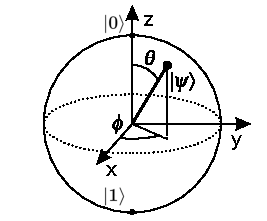
\includegraphics[width=.28\linewidth]{figures/BlochSphereCropped.pdf}
	\caption{The Bloch sphere representation. A classical bit can only be $\ket{0}$ or $\ket{1}$, whereas a qubit can occupy any point on the sphere with coordinates $\theta, \phi$. Figure adapted from \cite{Jones2012}.}
	\label{fig:BlochSphere}
\end{figure}

\subsection{Entanglement}\label{sub:Entanglement}

We will extend from 1 to 2 electrons. Now, they can be independently spin up $\ket{0}$ and down: $\ket{1}$, for a total of 4 basis states. Quantum physics teaches us this system can be in a superposition of all its basis states \cite{Nielsen2011}:

\begin{equation}\label{eq:TwoQubits}
	\ket{\psi_{2q}} = 
	\alpha_{00} \ket{00} + \alpha_{01} \ket{01} + \alpha_{10} \ket{10} + \alpha_{11} \ket{11}.
\end{equation}

Where $\ket{00}$ is a shorthand notation for both qubits being in the spin-up state, etc. In general, the size of the Hilbert space will grow as $2^N$ for $N$ qubits \cite{Henriet2020,Nielsen2011}. For $N=300$, this is already larger than the estimated amount of particles in the observable universe at some $\sim 10^{80}$. However, to access the full Hilbert space, the qubits need to be entangled. These are an inherent quantum feature, having no classical analog. One of the most instructive examples of an entangled state is 

\begin{equation}\label{eq:Entangled}
	\ket{\Phi^+} = \frac{1}{\sqrt{2}} \ket{00}+ \frac{1}{\sqrt{2}} \ket{11}
\end{equation}

This is one of the so-called Bell states \cite{Nielsen2011} and it is said to be entangled: upon measuring just one of the qubits we immediately know the state of the other qubit as well. This implies the qubits are correlated and cannot be described as a product of independent single qubits. In the operation of a quantum computer, entanglement is a crucial step during the computation stage \cite{Henriet2020}. 

\section{The NISQ Era}

Apart from controlling the quantum states of individual qubits, qubits are to be shielded from the environment, as noise from the environment can change the quantum states of the qubits.  This effect is known as decoherence \cite{DiVincenzo2000}. Decoherence errors can be corrected but this requires significant overhead in the available number of qubits and is unachievable in the near term \cite{Peres1985,Ladd2010}. Therefore, quantum computing is currently said to be in the \ac{NISQ} \cite{Preskill2018}. During the \ac{NISQ} era, the algorithms that run on quantum computers should be optimized for finite coherence times and fidelities. One algorithm proposed by \cite{Peruzzo2014} is thought to run especially well on non error-corrected hardware, so we will briefly describe its basic principle here \cite{McClean2016}. 

\subsection{The Variational Quantum Eigensolver}

The \ac{VQE} is a hybrid quantum algorithm: by making use of classical hardware it aims to reduce the number of quantum gates needed, which is advantageous on NISQ era hardware with finite coherence times \cite{McClean2016}. Essentially, \ac{VQE} tries to find approximately the ground state energy of an atom or molecule according to the variational principle \cite{Griffiths2004}, which states that the expectation value of a given Hamiltonian $\mathcal{H}$ will always be an upper bound for the ground state energy $E_g$:

\begin{equation}\label{eq:VariationalPrinciple}
	\left\langle \mathcal{H} \right\rangle = \bra{\Psi}\mathcal{H} \ket{\Psi} \geq E_g.
\end{equation}

This is equivalent to finding the eigenvalues of the matrix $\mathcal{H}$. Even for relatively simple molecules, $\mathcal{H}$ quickly becomes large and the task op diagonalizing it intractable, at least for a classical computer. In \ac{VQE}, $\mathcal{H}$ is not directly diagonalized but the Hamiltonian is prepared in a quantum co-processor or \ac{QPU} \cite{Henriet2020,Peruzzo2014}, taking advantage of the large Hilbert state of the quantum hardware. Given an ansatz $\theta$, a trial state $\ket{\Psi(\theta)}$ is prepared. The Hamiltonian is written in the form of a sum of Pauli strings: $P_{\alpha}$ with weights $h_{\alpha}$ \cite{McClean2016,Moll2018}

\begin{equation}\label{eq:PauliDecomposition}
	\mathcal{H} = \sum_{\alpha} h_{\alpha} P_{\alpha}
\end{equation}

\begin{figure}
	\centering
	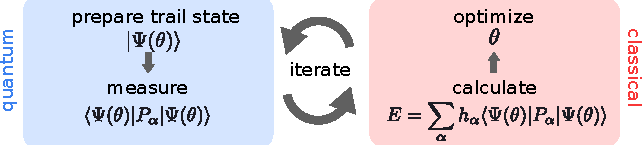
\includegraphics[width=0.75\linewidth]{figures/VQE.pdf}
	\caption{The \ac{VQE} visualized. Meant to run on a hybrid quantum computer, starting from an ansatz for the wave function it is prepared and the expectation function of its energy measured by a series of measurements on the \ac{QPU}. Next, a CPU uses a non-linear optimization to find a new ansatz that will decrease the expectation value of $\mathcal{H}$. Iterated until convergence. Figure adapted from \cite{Moll2018}}
	\label{fig:VQE}
\end{figure}

The Pauli string is essentially a tensor product of Pauli spin matrices, the definition is given in appendix \ref{ch:PauliExpectation}. Because of the decomposition in Pauli strings, estimating the various terms of the Hamiltonian $\bra{\Psi} P_{\alpha} \ket{\Psi}$ boils down to measuring populations of individual qubits, this is explained in appendix \ref{ch:PauliExpectation}. The total expectation value of the Hamiltonian is obtained by summing over contributions of the Pauli strings. This is done on classical hardware. Subsequently, a non-linear optimizer is run to minimize the energy using a new trial state, which is fed back into the \ac{QPU}. \cite{Moll2018}. The algorithm is visualized in \cref{fig:VQE}. The quantum and classical components of the algorithms feed into each other, therefore \ac{VQE} is referred to as a hybrid algorithm. 

\subsection{Hardware Implementation}

There are many options for implementing the algorithm on quantum hardware. \cite{DiVincenzo2000} formulated a list of criteria the hardware is to adhere to. Based on this, several quantum computer realizations have been proposed \cite{Ladd2010}. Examples include infrared photons \cite{Matthews2009},  trapped ions \cite{Benhelm2008,Schindler2013}, electron spins \cite{Press2008} and superconducting currents \cite{DiCarlo2009,Arute2019}. 

Another implementation is to use qubits encoded in the electronic states of neutral atoms. These atoms are assembled in arbitrary geometries using laser cooling and trapping techniques. One of those techniques is using tightly focused laser beams to trap atoms, also known as optical tweezers. This technique is thought to easily scale to a higher number of qubits by increasing the trapping laser power \cite{Henriet2020}. The atoms are held in place by optical dipole traps \cite{Chu1986}, each trap is non-deterministically loaded with single atoms \cite{Schlosser2001}. Multiple dipole traps spaced a couple of micrometers from each other are made using holography techniques \cite{Bergamini2004}. Interactions between qubits are realized using excitation to very high principle quantum numbers (Rydberg states) \cite{Levine2018,Madjarov2020}. Lastly, projections of qubit states are measured using laser induced fluorescence. An overview of the different steps in neutral atom quantum computing is shown in \cref{fig:ComputingSteps}.

\begin{figure}
	\centering
	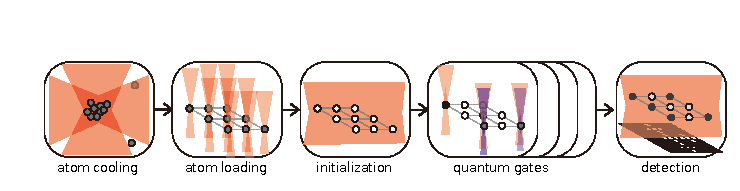
\includegraphics[width=\linewidth]{figures/ComputingSteps.pdf}
	\caption{Steps involved in running a \ac{QPU} based on neutral atoms in optical tweezers. Figure from \cite{Wu2021}.}
	\label{fig:ComputingSteps}
\end{figure}

\section{This Thesis}

In a collaboration with the \textit{Schreck} group, we aim to realize a \ac{QPU} based on strontium (Sr) atoms, which was recently shown to achieve high-fidelity quantum gates and measurements \cite{Madjarov2020}. The purpose of this thesis is to give an update of the first steps carried out in our group towards this goal. Therefore, this work is mostly about the first two steps in \cref{fig:ComputingSteps}. To to this the work is organized in the following way:

\begin{itemize}
	\setlength\itemsep{-1pt}
	\item Background information about laser cooling and trapping techniques, as well as for Sr specifically is presented in \cref{ch:coolingtrapping}. 

	\item Chapter \cref{ch:tweezer} is about focusing a laser beam to the smallest possible spot inside of a vacuum chamber, to realize an optical tweezer.

	\item Chapter \ref{ch:arrays} elaborates on how to make arrays of tweezers in arbitrary geometries by using holography techniques.

	\item Finally, in \cref{ch:implementation} we describe how to implement the setup in an ultracold experiment. Because the Sr atom source and laser system is set to arrive after this thesis was completed, we show progress towards trapping rubidium (Rb) instead, but the tweezer platform should work for Sr as well. 
\end{itemize}












\chapter{Laser Cooling and Trapping}\label{ch:coolingtrapping}
    In assembly, computation, and readout of single atoms, laser cooling and trapping techniques play a central role. This chapter will give some background on how this technique works, and how we intend to apply it onto strontium (Sr).
%stress difference between near-resonant regime dominated by scattering 2 level and off-resonant

\section{Magneto-Optical Trap}

The workhorse for producing clouds of ultracold atoms is the 3D \ac{MOT}. In essence, it consists of three sets of counter-propagating beams as well as a magnetic field gradient, together providing a dampening as well as a confining force. 

\subsection{Doppler Cooling}

Consider an atom with ground state $\ket{g}$ and excited state $\ket{e}$ separated by energy splitting $\hbar \omega_0$. This convention will be used for the remainder of this work. We drive a laser with omega $\omega$ that is near-resonant, but \emph{detuned} slightly from the transition by an amount $\delta$:

\begin{equation}\label{detuning}
	\delta = \omega - \omega_0
\end{equation}

It will turn out that detuning is one of the most important parameters in laser cooling. In this work we will always have $\delta <0$. Because of the Doppler effect, the atom 'sees' a slightly different light frequency depending on its velocity $v$ according to $\delta'=\delta+kv$ and the laser may become resonant: $\delta' = \omega_0$, causing the atom to absorb a photon absorbing momentum $\hbar k$ and promoting an electron to the excited state $\ket{e}$. When spontaneous emission causes the atom to fall back in a time $\tau = 1/\gamma$ where $\gamma$ is the linewidth of the transition, the electron is decayed back to the ground state, but the emitted photon is emitted in a random direction. This can be repeated many times per second at a scattering rate $\Gamma_{\text{sc}}$ \cite{Metcalf1999}

\begin{equation}\label{eq:ScatteringFrequency}
	\Gamma_{\text{sc}} = \frac{ \gamma s_0 /2}{1+s_0+\left[2(\delta+ k v)/\gamma\right]^2},
\end{equation}

where $s_0 = I/I_{sat}$ is the saturation parameter as a function of the light intensity $I$ for saturation intensity $I_{sat} = \hbar c \gamma \pi/3\lambdaup^3$ for wavelength $\lambda$ and linewidth $\gamma$. Because the absorption occurs in a fixed direction and the emission is a random event, the atom will experience a net force scattering force $F = \hbar k \Gamma_{sc}$.

\subsection{Optical Molasses}

We can reflect the laser beam using a mirror, such that the force works in both directions of the spatial coordinate. We will only consider one spatial coordinate which we will denote as $z$, but the treatment can be easily extended to 3 dimensions. The total force from both contributions from \cref{eq:ScatteringFrequency} is \cite{Kowalski2010}

\begin{equation}\label{eq:OpticalMolasses}
	F = \frac{\hbar k \gamma s_0}{2}\left\{\
	\left[1 + s_0 + 4\frac{(\delta+kv)^2}{\gamma^2}\right]^{-1}+
	\left[1 + s_0 + 4\frac{(\delta-kv)^2}{\gamma^2}\right]^{-1}
	\right\}
\end{equation}

We have plotted the result of \cref{eq:OpticalMolasses} in \cref{fig:MOTcooling} as a function of velocity in units of $\hbar / k$, such that it is dimensionless. Contributions of both beams, as well as their total force, are shown in units of $\hbar k \gamma$. Doing a series expansion to first order around $v = 0$. For $\delta<0$ we find we can linearize the force $F$ as \cite{Metcalf1999}

\begin{figure}
	\begin{subfigure}{.42\textwidth}
		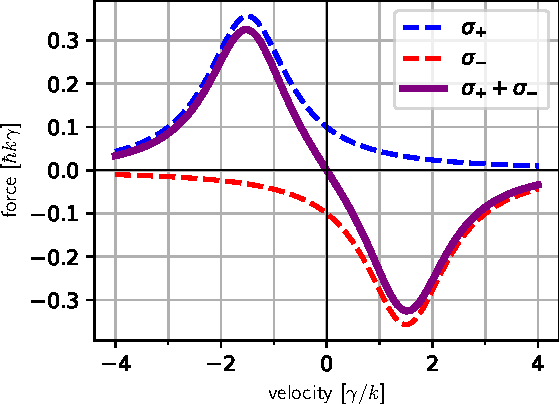
\includegraphics[height=4.5cm]{figures/MOTplot.pdf}
		\caption{}
		\label{fig:MOTcooling}
	\end{subfigure}
	\hfill
	\begin{subfigure}{.55\textwidth}
		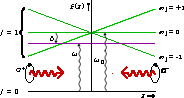
\includegraphics[height=4.5cm]{figures/OpticalMolasses.pdf}
		\caption{}
		\label{fig:MOTconcept}
	\end{subfigure}
	\caption{\textbf{a)} Cooling force from a magneto-optical trap. Contributions from the $F^+$, $F^-$ and the total force are shown for $\delta = -\gamma$ and $I/I_0 = 2.$ \textbf{b} Concept of optical molasses in 1D. Atomic frequency is detuned from the atomic transition by $\delta<0$. Because of the linear magnetic field, for $z>0$, the $m_j=-1$ atoms become resonant with only $\sigma^+$ light because of selection rules, and vice versa.}
	\label{fig:MOTPlots}
\end{figure}

\begin{equation}\label{eq:ForceLinearized}
	F \sim - \hbar k^2 s_0 \frac{-2\delta/\gamma}{\left[1+s_0+(2\delta/\gamma)^2\right]^2} \equiv -\beta v
\end{equation}

Where $\beta$ is the slope of the scattering force around $v=0$. The resulting force has a dampening character on the velocity, which if applied in all 3 dimensions can cool atoms to ultracold temperatures. 

The treatment so far would suggest that this can be used to cool atoms to temperatures of absolute zero. This is not the case, as the random character of the scattering force means the atom fluctuates around the equilibrium velocity according to a Brownian motion. 
%balance betweeen cooling and recoil heating. For higher s0 it is doppler broadened by a factor 
For $\delta=-\gamma/2$, \cref{eq:ForceLinearized} ($\beta$) is at a maximum, yielding the lowest possible temperature achievable using Doppler cooling: the Doppler temperature $T_D$ \cite{Metcalf1999}

\begin{equation}\label{eq:DopplerTemperature}
	T_D = \frac{\hbar}{2k_b} \gamma.
\end{equation}

where $k_b$ is Boltzmann's constant. Apparently, this cooling limit is only dependent on the linewidth of the transition $\gamma$, apart from physical constants. This result will be used later in \cref{sec:Sr}.

\subsection{Magnetic Trapping}

Apart from cooling the atoms, we want to trap them at a specific location to increase the density of atoms. We can use the Zeeman effect for this, which tells us the atomic energy levels will be split an amount $\Delta E$ according to \cite{Griffiths2004}

\begin{equation}\label{eq:Zeeman}
	\Delta E = \mu_{\emph{B}} g_J m_j B,
\end{equation}

where $\mu_{\emph{B}}$ Bohr magneton, $g_J$ the Landé g-factor, $m_j$ is the magnetic quantum number and $B_{\text{ext}}$ the applied magnetic field. The magnetic field is tuned in such a way that it is linear in all 3 dimensions and zero at the center of the \ac{MOT} by using a set of magnetic field coils in an anti-Helmholtz configuration. Because of the Zeeman splitting, the chance of the atoms coming in resonance with the laser varies with the position from the origin according to \cite{Kowalski2010}

\begin{equation}\label{eq:DetuningFull}
	\delta' = \delta + k v - \frac{\mu'B}{\hbar}
\end{equation}

Where $\mu' = (g_e m_e-g_g m_g)\mu_B$ is the effective magnetic moment for the transition \cite{Kowalski2010}. To ensure that atoms only absorb momentum kicks in the right direction, the laser beams are circularly polarized: $\sigma^+$ from the left and $\sigma^-$ from the right. Because the sign of the Zeeman shift is dependent on the magnetic quantum number $m_j$, selection rules prescribe that atoms displayed by $z>0$ are only resonant with $\sigma^-$-light and vice versa. This is sketched in \cref{fig:MOTconcept}. Inserting \cref{eq:DetuningFull} in \cref{eq:OpticalMolasses} yields

\begin{equation}\label{eq:MOTfull}
	\frac{F}{\hbar k \gamma s_0} = \frac{1}{2}\left\{\
	\left[1 + s_0 + 4\frac{(\delta+kv+\mu'B/\hbar)^2}{\gamma^2}\right]^{-1}+
	\left[1 + s_0 + 4\frac{(\delta-kv-\mu'B/\hbar)^2}{\gamma^2}\right]^{-1}
	\right\}
\end{equation}

Expanding \cref{eq:MOTfull} around $(v,z) = (0,0)$, keeping only first order terms finally leaves us with \cite{Kowalski2010}

\begin{equation}\label{eq:ForceMOT}
	F_{\text{MOT}}(z,v) \sim -\beta v - \kappa z.
\end{equation}

Where $\beta$ is the same we found in \cref{eq:ForceLinearized} and $\kappa \equiv \mu' \beta /\hbar k \cdot \partial B/\partial z$. Apart from the dampening force, we now also have a restoring force. When applied in 3 dimensions this can be used to make clouds of ultracold atoms. 

\section{Optical Dipole Traps}\label{sec:OpticalDipoleTrap}

While magneto-optical traps are excellent for producing clouds of ultracold atoms, the constant photon scattering is unwanted during qubit operation. Therefore, after the atom cloud is cooled in the \ac{MOT}, it is typically loaded in another type of trap: the \ac{ODT}. An ODT uses far-off-resonant light. Though this means that the coupling and therefore the trapping is weaker, it has negligible scattering, which is important to maintain coherence of quantum states. We consider a radiation field $\mathbf{E}$. This field will induce a dipole moment $\mathbf{p}$ in the atom according to 
	
\begin{equation}\label{eq:DipoleMoment}
	\mathbf{p} = \alpha \mathbf{E}.
\end{equation}

Consequently, the dipole potential will interact with the electric field leading to and an interaction dipole potential $U_{\text{dip}}$ as a function of the position vector $\mathbf{r}$ \cite{Grimm2000}

\begin{equation}\label{eq:DipolePotential}
	U_{\text{dip}}(\mathbf{r}) = -\mathbf{p}\mathbf{E} = 
	-\frac{1}{2} \left\langle \mathbf{p}\mathbf{E} \right\rangle = \frac{\operatorname{Re}(\alpha)}{2\epsilon_0 c} I(\mathbf{r}),
\end{equation}

where the $\left\langle\right\rangle$ brackets denote the time average. We average over this radidly varying phase term, yielding a factor $1/2$. Furthermore we used $I(\mathbf{r}) = |\mathbf{E}(\mathbf{r})|^2/(2\epsilon_0 c)$ where $\epsilon_0$ is the electric constant. The dipole force thus scales with the in-phase part of the polarizability with the light field. An additional factor $1/2$ comes in because the dipole moment is induced and not permanent \cite{Grimm2000}. The gradient of \cref{eq:DipolePotential} gives rise to the dipole force:

\begin{equation}\label{eq:DipoleForce}
	\mathbf{F}_{\text{dip}}(\mathbf{r}) = - \frac{\operatorname{Re}(\alpha)}{2\epsilon_0c}\nabla I(\mathbf{r})
\end{equation}

The dipole force can be used to coherently trap our qubits. To maximize the dipole force \cref{eq:DipoleForce}, we have to maximize the gradient of the light intensity profile. This can be done by focussing the laser on the smallest possible spot. How we do this is explained in \cref{ch:tweezer}. The scattering rate from the ODT can be found by averaging over the derivative of the dipole moment with the electric field \cite{Grimm2000}

\begin{equation}\label{eq:ScatteringRate}
	\Gamma_{\text{sc}}(\mathbf{r}) = \frac{\left\langle \mathbf{p} \mathbf{E} \right\rangle}{\hbar \omega}
	 = \frac{\operatorname{Im}(\alpha)}{\hbar \epsilon_0 c} I(\mathbf{r}).
\end{equation}

\cref{eq:DipoleForce,eq:ScatteringRate} are general expressions for any potential. The fact that $\alpha(\omega)$ is complex means there is a phase delay between the electric field and the dipole response. The task that remains is finding the polarizability $\alpha(\omega)$. As a starting point, we will consider the electron as a (classical) damped harmonic oscillator, which is for Alkali species already fairly accurate \cite{Grimm2000}.

\subsection{Classical}

In the classical picture, we assume a classical light field, as well as a classical electron (harmonic oscillator). We can write down a general expression for the the light field propagating in the $z$-direction polarized in the $\bm{\hat{\epsilon}}$ direction perpendicular to it:

\begin{equation}\label{eq:ClassicalField}
	\mathbf{E}(z,t) = \mathbf{E}_0 \cos{(k z - \omega t)} 	\bm{\hat{\epsilon}}
\end{equation}
	 
The electron is modeled as a damped harmonic oscillator (Lorentz oscillator). Integrating the equation of motion for the electron, assuming a dipole moment $\mathbf{p} = e \mathbf{r}$ where $r$ is the position yields after equating to \cref{eq:DipoleMoment} for the polarizability \cite{Grimm2000}

\begin{equation}\label{eq:LorentzOscillator}
	\alpha(\omega)=6 \pi \epsilon_{0} c^{3} \frac{\Gamma / \omega_{0}^{2}}{\omega_{0}^{2}-\omega^{2}-\mathrm{i}\omega^3\Gamma/\omega_0^2}
\end{equation},

Where $\Gamma$ is the on-resonant damping rate in terms of the electron mass $m_e$. 

\begin{equation}\label{eq:ResonantDampingRate}
	\Gamma = \frac{e^2 \omega_0^2}{6\pi \epsilon_0 m_e c^3}
\end{equation}

Inserting \cref{eq:LorentzOscillator} in \cref{eq:DipolePotential,eq:ScatteringRate} yields, after assuming $\delta \ll \omega, \Gamma \ll \omega$

\begin{equation}\label{eq:DipoleClassicalResult} 
	U_{\text{dip}}(\mathbf{r}) = 
	\frac{3\pi c^2}{2\omega_0^3}\frac{\Gamma}{\delta} I(\mathbf{r}),
	\quad
	\Gamma_{\text{sc}}(\mathbf{r}) = 
	\frac{3\pi c^2}{2\hbar\omega_0^3}\left(\frac{\Gamma}{\delta}\right)^2 I(\mathbf{r})
\end{equation}

From \cref{eq:DipoleClassicalResult} the relation these two quantities is $\hbar \Gamma_{sc} =\Gamma U_{\text{dip}}/\delta$. Thus, to keep scattering events to a minimum a large detuning should be used. To still have sufficiently deep traps, high light intensities are used. 


\subsection{Semi-Classical}

In the semi-classical picture, we consider the same classical light field \cref{eq:ClassicalField}, but consider an atom with quantized energy levels. We will consider a two-level atom with eigenstates $\ket{g}$ (ground) with energy $\hbar \omega_g$ and $\ket{e}$ (excited) with $\hbar \omega_e$, see \cref{fig:2LevelAtom}. Then the atomic Hamiltonian in this basis reduces to \cite{Loudon2000}

\begin{figure}
	\centering
	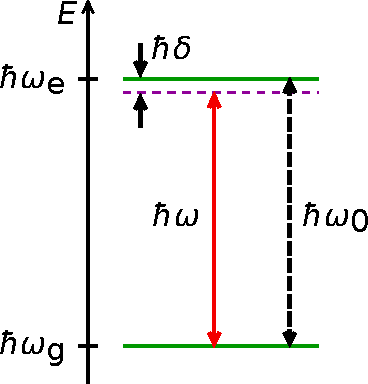
\includegraphics[height=4.1cm]{figures/2LevelAtom.pdf}
	\caption{Energy level scheme for the 2-level case. The two energies are split by $\omega_e - \omega_g = \omega_0$. The detuning is $\delta = \omega-\omega_0<0$ is shown as well.}
	\label{fig:2LevelAtom}
\end{figure}

\begin{equation}\label{eq:AtomHamiltonianMain}
	\mathcal{H}_A = \hbar \omega_g \ket{g}\bra{g} + \hbar \omega_e \ket{e}\bra{e}
\end{equation}

The radiation field is modeled as a time-dependent perturbation such that the total Hamiltonian is \cite{Leeuwen2017}

\begin{equation}\label{eq:PerturbationMain}
	\mathcal{H} = \mathcal{H}_A + \mathcal{H}_{I}(t),
\end{equation}

We can write down the combined wave function in the basis of the unperturbed eigenstates, its time evolution given by

\begin{equation}\label{eq:TwoLevelMain}
	\ket{\psi(t)} = c_g(t) e^{-i \omega_g t} \ket{g} + c_e(t) e^{-i \omega_e t} \ket{e}.
\end{equation}

In appendix \ref{ch:LightMatter} the Schrodinger equation is solved for the 2-level atom using the dipole approximation as well as the \acf*{RWA}. The following matrix equation is derived for the 2 level atom (\cref{fig:2LevelAtom}) \cite{Foot2005}

\begin{equation}\label{eq:MatrixEvolution}
	i \hbar \begin{pmatrix}
		\dot{c}_g \\ 
		\dot{c}e
	\end{pmatrix}
	= \frac{\hbar}{2} \begin{pmatrix}
		\delta & \Omega \\ \Omega^* & -\delta 
	\end{pmatrix} 
	\begin{pmatrix}
		c_g \\ c_e,
	\end{pmatrix}
\end{equation}.

where the coupling between the atomic eigenstates and the radiation field is described by the Rabi frequency \cite{Metcalf1999}:

\begin{equation}\label{eq:RabiFrequencyMain}
	\Omega \equiv \frac{e E_0}{\hbar} \bra{g}\mathbf{r}\ket{e}.
\end{equation}

The Hamiltonian of \cref{eq:MatrixEvolution} has eigenvalues 

\begin{equation}\label{eq:EigenValues}
	E_{\pm} = \pm
	\frac{\hbar}{2} \sqrt{\Omega^2+\delta^2}.
\end{equation}

Assuming $|\delta| \gg \Omega$, the eigenenergies are thus 

\begin{equation}\label{eq:SemiClassicalEigenvalues}
	E_g \sim  \frac{\hbar \delta}{2} +\frac{\hbar \Omega^2}{4 \delta}, \quad
	E_e \sim -\frac{\hbar \delta}{2} -\frac{\hbar \Omega^2}{4 \delta}
\end{equation}

When turning on the laser, the energies are thus shifted by an amount $\Delta E = E(\Omega)-E(\Omega=0)$. This is called the light shift or AC Stark shift \cite{Metcalf1999}, sketched in \cref{fig:DipoleForce}.

\begin{figure}
    \centering
	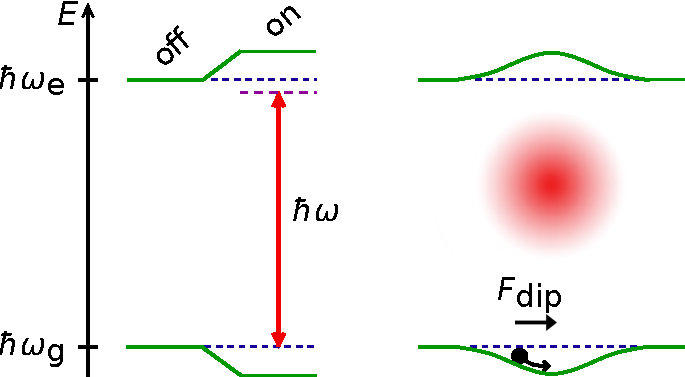
\includegraphics[height=3.8cm]{figures/LightShift.pdf}
	\caption{Light shift when the off-resonant laser is turned on, as well as the spatially varying light shift for a laser beam profile for $\delta<0$. Figure not to scale.}
	\label{fig:DipoleForce}
\end{figure}

\begin{equation}\label{eq:Stark}
	\Delta E_{e,g} \sim \pm \frac{\hbar \Omega^2}{4 \delta}.
\end{equation}

The light shift is proportional to the light intensity over the detuning: $\Omega^2 / \delta \propto I / \delta$, which we already found for the classical treatment in \cref{eq:DipoleClassicalResult}. This behavior of \cref{eq:Stark} is shown in \cref{fig:DipoleForce}. Because the field is off-resonant, atoms only occupy the ground state. For $\delta <0$ ('red detuned'), the ground state light state is negative. To calculate the new eigenstates, we repeat the treatment for a quantized light field. This is known as the dressed atom picture.

\subsection{Dressed Atom Picture}\label{sec:DressedApproach}

To calculate the new shifted eigenstates, the full Hamiltonian has to be considered, included a quantized light field with Hamiltonian $\mathcal{H}_L$ \cite{Dalibard1985}

\begin{equation}
	\mathcal{H} = \mathcal{H}_A + \mathcal{H}_L + \mathcal{H}_I(t)
\end{equation}

where the light field has eigenenergies separated by the photon energy and eigenstates of $n$ photons: $\ket{n}$ \cite{Vredenbregt2020}

\begin{equation}\label{eq:RadiationModes}
	\mathcal{H}_L = \sum_n \hbar \omega \left(n+\frac{1}{2}\right) \ket{n}\bra{n}
\end{equation}

The eigenmodes of the light field can only couple to one energy pair of the $\mathcal{H}_A + \mathcal{H}_I$ part, such that the Hamiltonian can be written down as a direct product of 2 x 2-matrix Hamiltonians \cite{Vredenbregt2020,Hussin2005} $\mathcal{H}_n$:

\begin{equation}\label{eq:CunningsHamiltonian}
    \mathcal{H}_n = \hbar 
    \begin{pmatrix}
        (n + 1)\omega -\omega_0 / 2                     & -\frac{1}{2}\sqrt{\Omega^2+\delta^2(n+1)} \\
        -\frac{1}{2}\sqrt{\Omega^2 + \delta^2(n+1)}  & n\omega + \omega_0/2
    \end{pmatrix}
\end{equation}

This is known as the Jaynes-Cummings Hamiltonian, which is one of the few problems in quantum optics analytically solvable. It has eigenvalues \cite{Hussin2005}

\begin{equation}\label{eq:CunningsEigenvalues}
    E_{\pm} = \hbar\omega\left(n+\frac{1}{2}\right) \pm \frac{\hbar}{2} \sqrt{\delta^2 + \Omega^2(n+1)}.
\end{equation}

Note the similarity to \cref{eq:SemiClassicalEigenvalues}. From \cref{eq:CunningsEigenvalues} the new eigenstates can be found to be \cite{Hussin2005}

\begin{subequations}\label{eq:CummingsEigenstates}
    \begin{align}
        \ket{+,n} &= \cos{({\theta_n}/2)} \ket{n+1,g} -\sin{(\theta_n/2)} \ket{n,e}, \\
        \ket{-,n} &= \sin{(\theta_n/2)}\ket{n+1,g} + \cos{(\theta_n/2)} \ket{n,e}.
    \end{align}
\end{subequations}

Which are sketched in \cref{fig:DipoleForce} as well. In \cref{eq:CummingsEigenstates} the mixing angle $\theta_n$ for $n$ photons in the system is $\theta_n = \arctan{(\Omega\sqrt{n+1} / \delta})$. Here, \cref{eq:CummingsEigenstates} are known as the \emph{dressed} states. The \emph{bare} atomic states in \cref{fig:2LevelAtom} are shifted by the light shift because the light field energy is admixed with the atomic eigenstates, leading to the new mixed (dressed) eigenstates of \cref{eq:CummingsEigenstates}. The bevavior pictured in \cref{fig:DipoleForce} still applies, but if the eigenenergies of the light field are included, the splitted energies of \cref{fig:DipoleForce} are situated along an infinite ladder of photon energies. This is presented in \cref{fig:DressedStatePicture}. The light space eigenenergies \cref{eq:RadiationModes}, spaced by $\hbar \omega$ is superimposed on the light shift eigenenergies. 

\begin{figure}
    \centering
    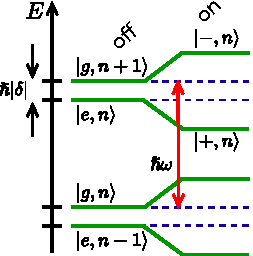
\includegraphics[width=0.3\linewidth]{figures/DressedStates.pdf}
    \caption{Dressed States. The same shift as shown in \cref{fig:DipoleForce} is shown, superimposed on the  eigenenergies spaced by $\hbar \omega$. Figue not to scale. }
    \label{fig:DressedStatePicture}
\end{figure}


\section{Strontium}\label{sec:Sr}

Historically, people started laser cooling experimentation on group 1 or alkali atoms (Na, Rb, Cs). Because they only have one valence electron, the level structure is relatively straightforward. Also, diode lasers are available for their transition frequencies. In this work, trapping of \textsuperscript{85}Rb (an alkali) is described in \cref{ch:implementation}.

However, also group 2 atoms, also called alkali-earth (and similar atoms like Yb) are possible candidates. Because of their two valence electrons, the level structure is much more complicated, making laser cooling harder, but possibly also opening up new possibilities. The element we wish to use for our new machine in Eindhoven is Sr. For more extensive coverage of Sr, the reader is referred to \cite{Stellmer2013}. Three of them are bosonic, with ${}^{88}$Sr being the most abundant at $\sim82.6\%$. There is one stable fermionic isotope: ${}^{87}$Sr has a nuclear spin of $I=9/2$ and an abundance of $\sim7.0\%$ \cite{Coursey1999}. Initially, we plan to run the machine in Eindhoven on \textsuperscript{88}Sr. Because of the lack of hyperfine structure, this isotype is a bit easier to work with, but in principle, one can use all isotopes in the same machine as the energy splitting between the isotopes is in the MHz regime, easily covered by AODs and EOMs \cite{Stellmer2013}.

\subsection{Relevant Transitions}

A simplified version of the level diagram of \textsuperscript{88}Sr is shown in \cref{fig:SrLevel}. The notation is $(n_1l_1 n_2l_2)^{2S+1}L_J$ where $n_{1,2}$ is the principal and $l_{1,2} = s, p, d, \ldots$ the azimuthal quantum number. Furthermore $S$, $L$ and $J$ are the total spin, orbital angular momentum, and total angular momentum respectively \cite{Cowan1981}.  This level scheme shows 6 out of 7 lasers to be used in this experiment. 

\begin{itemize}
	\item 461 nm. Broad transition, meaning a strong scattering force (\cref{eq:ScatteringFrequency} and high aborption-emmision cycling frequency. This is useful to slow down the hot atomic beam coming from the oven, as well as catching the atoms in a so-called blue \ac{MOT} with 'hot' temperatures of $\sim$ 1 mK.)
	
	\item 689 nm. Being much narrower than the blue transition, its Doppler temperature \cref{eq:DopplerTemperature} is much lower at $179$ nK, although in practice cooling is limited by the recoil limit to some $\sim 1$ $\mu$K \cite{Stellmer2013,Boyd2007}.
	
	\item 698 nm. The ultra-narrow clock transition ($\gamma = 1$ mHz). Used in atomic clocks because of its spectroscopic accuracy \cite{Bloom2014}. It will turn out that this feature can be put to good use in quantum computers as well, and we will use it to coherently 'drive' the qubits between the qubit basis states using this clock transition. More about this in \cref{sec:QubitScheme}
	
	\item 679, 688, and 707 nm. All repump lasers. 707 and 688 are used to cycle back atoms from ending up in ${}^3P_2$ from the decay channel shown by the grey dotted line in \cref{fig:SrLevel}. 679 is used to prevent repump leaks to ${}^3P_0$ \cite{Stellmer2013,Xu2003}.
\end{itemize}

There will also be a 813 nm laser used for the dipole trapping. This is also the most powerful laser, as it determines the limit of optical dipole traps (optical tweezers) one can make. More about this transition in \cref{sec:Magic}.

\begin{figure}
	\centering
	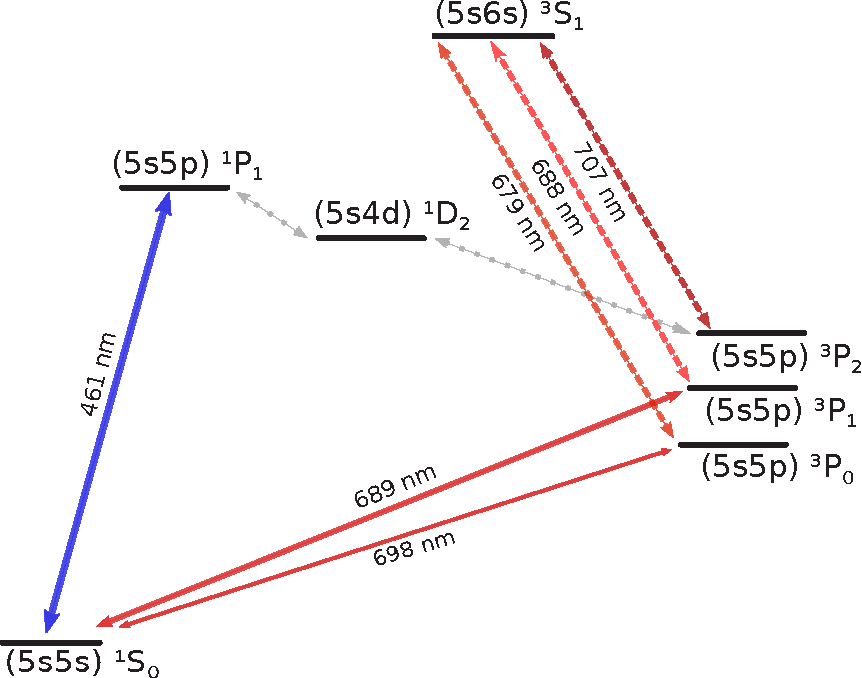
\includegraphics[width=0.55\linewidth]{figures/SrLevel.pdf}
	\caption{Simplified level scheme for \textsuperscript{88}Sr. Shown: blue transition for initial slowing and cooling. Narrower 689 nm transition of the red \ac{MOT}, and the \textsuperscript{1}S\textsubscript{0} - \textsuperscript{3}P\textsubscript{0} clock transition, which we will be used to drive the qubits. To increase density and trap lifetime 3 repump lasers are used. Not shown: 813 nm dipole trapping laser because it is driven far-off-resonant. Energies not to scale. Figure made by Ivo Knottnerus.}
	\label{fig:SrLevel}
\end{figure}

\subsection{Laser Cooling and Trapping of Sr}

Because the melting temperature of Sr is $777$ ${}^{\circ}$C, to get any relevant vapor pressure, the Sr is heated in an oven after which it sublimates. To obtain a small atomic beam divergence, the atoms are directed through a bundle of high aspect ratio capillary tubes \cite{Stellmer2013}. 

Because of the oven, the atoms are moving way too fast to be efficiently captured by the MOT. Therefore, they are slowed by a Zeeman slower. This machine uses a similar design used in the optical molasses technique, only the slowing beam is only opposing the atomic beam and not traveling along with it. A spatially varying magnetic field ensures a wide range of velocities is at some point resonant with the laser according to \cref{eq:DetuningFull}. 

Depending on the length of the Zeeman slower, only a fraction of the atoms will be slowed. To separate the hot from the cool atoms (the former are unwanted in a vacuum chamber) a deflection stage is used. The blue transition of Sr is used for this stage because of the strong scattering force. The Zeeman slowing and deflection stage is explained more elaborately in the thesis of Rik van Herk \cite{Herk2022}.

After the deflection stage, the atomic beam enters a glass cell. The advantage of using a glass cell is that it allows for the maximum amount of optical axis. To allow for longer trap survival times, the glass cell has \ac{UHV} which is separated from the stages preceding it by a differential pumping stage. 

\begin{figure}
	\centering
	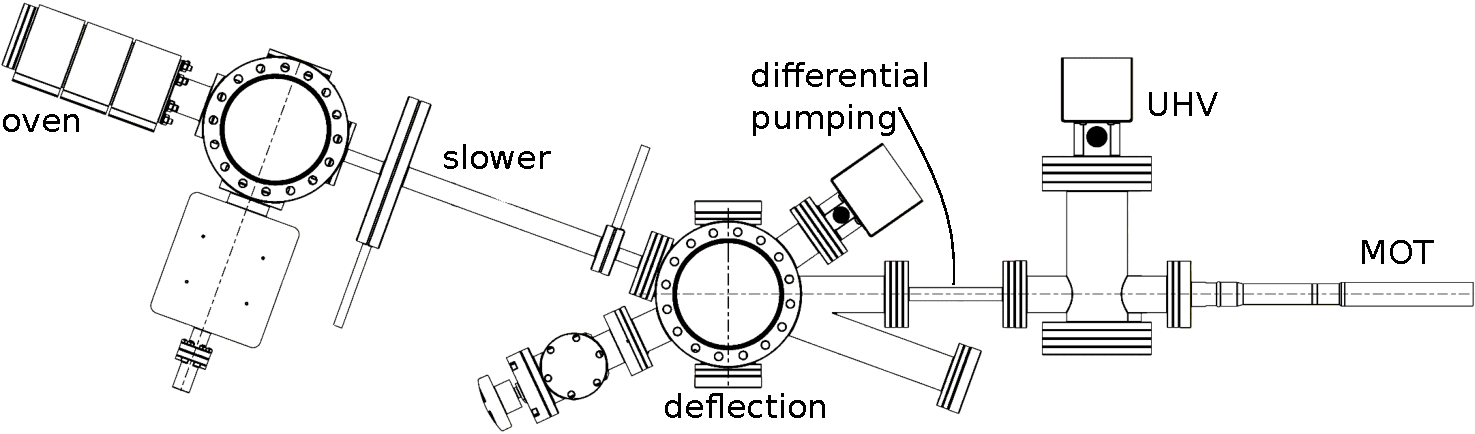
\includegraphics[width=0.8\linewidth]{figures/SrLoading.pdf}
	\caption{Sketch of the vacuum atom source design and vacuum chambers. Starting from the oven, the atomic beam traverses a Zeeman slower, deflection stage, and differential pumping stage before ending in the glass cell (MOT, right). The author did not contribute to this design. Figure by Patrick de Laat.}
	\label{fig:SrLoading}
\end{figure}

\subsection{Strontium as a Qubit}\label{sec:QubitScheme}

One of the main reasons we want to use strontium atoms for the quantum processing unit is the ${}^3P_0$ state and its very long lifetime. The clock transition is forbidden according to selection rules and only opens up after applying a magnetic field for the \textsuperscript{88}Sr isotope. Therefore,  ${}^3P_0$ is called meta-stable and can be considered a ground state on the time scale of the operation of a quantum processing unit. ${}^1S_0$ is the other clock state. Therefore, we effectily have two ground states and we can denote our qubit states as $\ket{g_1}$ and $\ket{g_2}$ (the clock states) as

\begin{equation}\label{eq:QubitManifold}
	\big\{\ket{0},\ket{1}\big\} = 
	\left\{
		\ket{{}^1S_0}, \ket{{}^3P_0} 
	\right\} = 
	\left\{ 
	    \ket{g_1}, \ket{g_2}
	\right\}.
\end{equation}

So we have two long-lifetime states connected by an extremely narrow linewidth coupling between them, that can be used to drive the qubits on the Bloch spheres. To entangle the qubits, Rydberg dressing can be used \cite{Wu2021} where a small part of a Rydberg state $\ket{r}$ is admixed in the higher energy ground state:

\begin{equation}\label{eq:RydbergDressing}
	\ket{\psi} \sim \ket{g_2} + \epsilon \ket{r}
\end{equation}

The amount of dressing is tuned by the (small) dressing parameter $\epsilon \propto \Omega / 2\delta$ where $\Omega$ is the Rabi frequency of the laser and $\delta$ the usual detuning. A Rydberg state is an electronic state with a very high principal quantum number $n$. Rydberg atoms are physically larger, as the electron orbit radius scales $\propto n^2$ \cite{Gallagher1994}. As a result of these exaggerated electron orbit sizes, neighboring atoms can 'feel' each other. For example, the van der Waals interaction coefficient scales as $\propto n^{11}$ \cite{Gallagher1994}. 

Other qubit implementations than the one above are possible as well. For example, \cite{Barnes2021} uses the fermionic ${}^{87}$Sr and maps the qubit states onto the nuclear spin states $\ket{{}^1S_0, F=9/2, m_F = -9/2}$ and $\ket{{}^1S_0, F=9/2, m_F = -7/2}$.

\subsubsection*{Magic Trapping of Strontium}\label{sec:Magic}

\begin{figure}
\centering
	\begin{subfigure}{.4\textwidth}
		\centering
		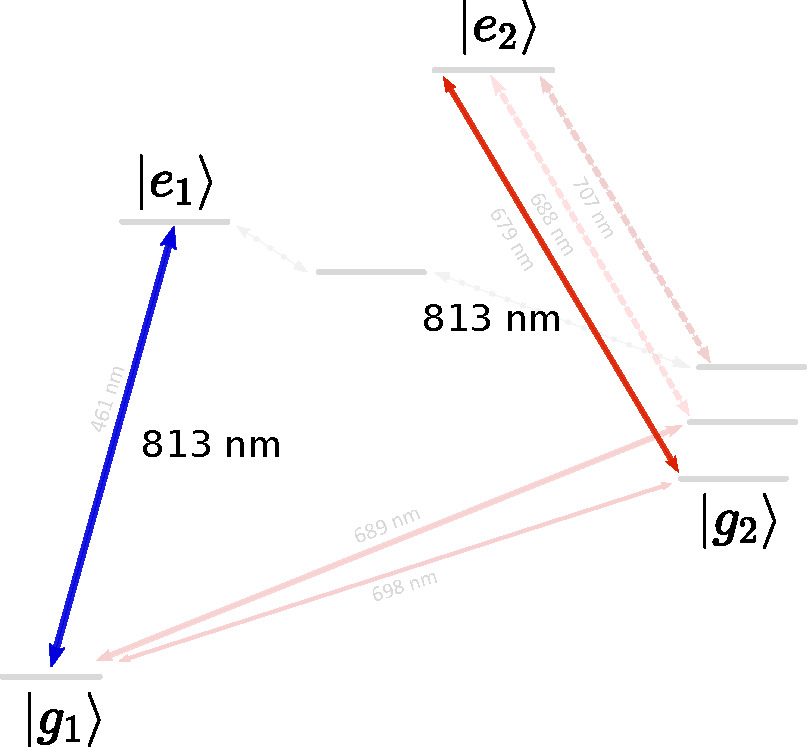
\includegraphics[height=5cm]{figures/2groundTweezer.pdf}
		\caption{}
		\label{fig:2LevelTweezer}
	\end{subfigure}
	\begin{subfigure}{.5\textwidth}
		\centering
		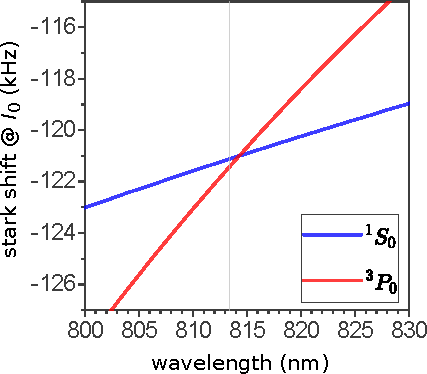
\includegraphics[height=5cm]{figures/Magic.pdf}
		\caption{}
		\label{fig:BoydMagic}
	\end{subfigure}
	\caption{\textbf{a)} Both clock states, here denoted $\ket{g_1}, \ket{g_2}$ are coupled to a different excited state: $\ket{e_1}, \ket{e_2}$ using the same trapping laser at 813 nm.\textbf{ b)} Atomic polarizabilities of ${}^1S_0$ and ${}^3P_0$ showing a magic crossing around 813 nm. Grey line: experimental result. Figure adapted from \cite{Boyd2007}.}
	\label{fig:GerschbergSaxton}
\end{figure}

To use the states in \cref{eq:QubitManifold} in a quantum processing unit, they should both be trapped. Because the trapping potential is wavelength dependent, in general, the trapping potential will not be the same for both qubit states when using the same trapping wavelength (\cref{eq:DipoleForce}: $U_{\text{dip}} \propto - \operatorname{Re}\{\alpha(\omega)\} I(\mathbf{r})$, meaning that the transition frequency between the qubit states would change as a function of the position within the potential which is unfavorable. Instead, \cite{Katori2003} proposed to use a wavelength where the polarizability $\alpha(\omega)$ or $\alpha(\lambdaup)$ is identical for both clock states as measured by \cite{Takamoto2005,Jun2008}.

Calculating this \textit{magic} crossing point of \cref{eq:MagicCrossing} is outside the scope of this thesis, but we will show the final result as found by \cite{Boyd2007} in \cref{fig:BoydMagic}. The reader is referred to \cite{Madjarov2020,Boyd2007} for more information. Plotting the polarizability for both clock states as a function of wavelength and one findes a magic crossing point around 813 nm. By trapping both qubit states in the same potential, one can coherently drive the qubits to any point on the Bloch spheres. 

Both qubit states coupled far-off-resonantly to a different excited states using this same magic potential. The excited states used can be found in \cref{fig:SrLevel}. That figure is one again plotted in \cref{fig:2LevelTweezer}, where the two different dipole trap schemes are highlighted.

\begin{equation}\label{eq:MagicCrossing}
    \operatorname{Re}\left\{\alpha(\lambdaup-\lambdaup_{\ket{g_1})})\right\} = 
    \operatorname{Re}\left\{\alpha(\lambdaup-\lambdaup_{\ket{g_2})})\right\}
\end{equation}





	



\chapter{Optical Tweezers}\label{ch:tweezer}
    The tool used in this work to achieve single-atom control is optical tweezers: by focussing a laser beam to a small enough spot it has been shown that under the right conditions, this trap can house at most one atom. 

\section{Loading Single Atoms}\label{sec:LoadingAtoms}

Single atom loading was first demonstrated by \cite{Schlosser2001}. 
Call the number of atoms in the tweezer $N$, \cite{Schlosser2002} suggested for the time-derivative of $N$ a model with contributions

\begin{equation}\label{LoadingTweezer}
	\frac{\text{d}N}{\text{d}t} = \alpha - \gamma N - \beta N(N-1)
\end{equation}

where the first term $\alpha$ is the loading rate or the amount of atoms entering the tweezer per second. 
Next, $\gamma$ is the atom loss as a result of collisions with the background gas. 
Lastly, $\gamma$ is a measure for the mainly 2 body loss as a result of light-assisted collisions.
3-body terms and higher are disregarded. 
In order to load single atoms, we must satisfy $\beta \gg \gamma$: the two-body collisions are dominant.
We can now look at two distinct scenarios:

\begin{itemize}
	\item Starting from 0 atoms in the tweezer: an additional atom entering will now load the tweezer to $N=1$. 
	
	\item Starting from $N=1$: when an additional atom is loaded, the atoms will immediately kick out each other because of the tiny tweezer volume and strong light intensity from the MOT beams. 
\end{itemize}

If the number of atoms at $t=0$ is larger than $N$, atoms will be lost in pairs until $N$ is either 0 or 1, after which the events above apply. 
Apparently, a loading event can lead to either 0 or 1 atom in the tweezer, both with $50\%$ probability. 
This is known as the collisional blockade effect. Experimentally demonstrated by \cite{Schlosser2001} and \cite{Schlosser2002} showed this effect to exits for 3 orders of magnitude in the loading rate $\alpha$.
Satisfying $\beta \gg \gamma$ can be done by keeping $\gamma$ to a minimum by going to the ultra high vacuum regime.
We intent to go to a pressure of the order of $10^{-10}$ mbar. In addition $\beta$ is maximized by going to high light-intensities and small trapping volumes. 
The remainder of this chapter is dedicated on how to minimize this trapping volume.

\section{Diffraction Limit}

The smallest achievable spot size is governed by the diffraction limit, which states that because light is a wave, it is impossible to focus down to an infinitely small spot even in the absence of aberrations.
Diffraction is elegantly described by Fourier optics \cite{Goodman2005}. 
We derive a result used throughout this work here.

\begin{mdframed}
    \subsection*{Intermezzo Fourier Optics}
    
    As we use the objective to make a tweezer, light is impinging on its back aperture. 
    We call its complex amplitude $U(x',y')$ and define the aperture at $z = 0$ on the optical axis.
    After the aperture, light will show diffraction. 
    An elegant description is provided by scalar diffraction theory.
    We will not repeat a full derivation here but we can refer the reader to \cite{Goodman2005}.
    Consider the Fresnel diffracion integral in cartesian coordinates. 
    After the aperture, the complex amplitude $U$ distribution is:
    
    \begin{equation}\label{eq:FresnelDiffraction}
        E(x,y,z) = 
        \frac{e^{ikz}}{i \lambda z} \iint_{-\infty}^{\infty} U(x',y',0) \exp{\frac{ik}{2z}} \exp{\left[(x-x')^2+(y-y')^2\right]} dx'dy'.
    \end{equation}
    
    In \cref{eq:FresnelDiffraction}, $\lambda$ is the wavelength, $k=2\pi/\lambda$ the wavenumber.
    In this thesis, we are usually not immediately interested in describing the light in the the near field of the aperture, but in the far-field. 
    More formally, the following needs to apply:
    
    \begin{equation}\label{eq:FraunhoferCriterion}
        z \gg k R^2/2,
    \end{equation}
    
    where $R$ is the maximum distance from the aperture to the optical axis. 
    While this criterion is in practice not met, it does hold in the focal point of a lens, because a lens projects an image in infinity to its focal length $f$. 
    Inserting \cref{eq:FraunhoferCriterion} in \cref{eq:FresnelDiffraction} yields:
    
    \begin{equation}\label{eq:FraunhoferDiffraction}
        E(x, y, z)=\frac{e^{i k z} e^{i k\left(x^{2}+y^{2}\right)/2}}{i \lambda z} \iint_{-\infty}^{\infty} U(x', y') \exp \left[\frac{-ik}{z}(x x'+y y')\right] dx' dy'
    \end{equation}. 
    
    This equation relates the field in the focus point point of the lens $U(x,y)$ to the field at the lens $U(x',y')$. 
    Contributins outside of the apeture can be discarded, and in practice we are not too intersted in the phase factor in front, such that we have
    
    \begin{equation}\label{eq:FraunhoferSimplified}
        E(x,y,z) \propto 
        \iint_{\text{aperture}} U(x',y') \exp{\left[- \frac{ik}{z}(xx'+yy')\right]}dx'dy'
    \end{equation}
    
    We recognize in \cref{eq:FraunhoferDiffraction} the spatial Fourier transform, in both $x$ and $y$ with respectively the frequencies $f_x = x/\lambda z$ and $f_y = y/\lambda z$, which is a result we will use later in this work. \cref{eq:FraunhoferDiffraction} is the Fraunhofer diffraction integral.
\end{mdframed}

 In this work, we are mostly concerned with circularly shaped apertures, for which a description in cylindrical coordinates is more natural.
 Ignoring the phase factor in front of the integral:

\begin{equation}\label{eq:FraunhoferRTheta}
    E(r,\theta, z) \propto \iint_{\text{aperture}} U(r') \exp{\left[
    -\frac{i k r r'}{z} \cos{(\theta-\theta')} 
    \right]}r'dr'd\theta'
\end{equation}

Using the integral definition of the Bessel function of the first kind\footnote{$J_0(x) = \frac{1}{2\pi} \int_0^{2\pi} \exp{(i x \cos{\alpha})} d\alpha$} we write \cref{eq:FraunhoferRTheta} as 

\begin{equation}\label{eq:FourierBessel}
    E(r,z) \propto 2\pi \int_0^{\infty} U(r') J_0\left( \frac{k r r'}{z}\right) r'dr'
\end{equation}

\cref{eq:FourierBessel} is the Fourier-Bessel or Hankel transform.
Now that the general formula has been derived, will make the problem more specific by introducing some parameters. 
In practice, we are interested in the focus point of the lens around $z \approx f$. 
We send a Gausian beam through the lens with an circular aperture function $U(r')$ with radius $R$, such that the input $E_i$ is

\begin{equation}\label{eq:GaussianAperture}
    E(r')=
    \begin{cases}
        e^{- w_i^2/R^2},& \text{if } r' < R\\
        0,               & \text{otherwise}
    \end{cases}
\end{equation}

Substituting \cref{eq:GaussianAperture} in \cref{eq:FourierBessel} yields

\begin{equation}\label{eq:FourierBesselAperture}
    E(r) \propto \int_0^R e^{-r'^2/w_i^2} J_0\left(\frac{k r r'}{f}\right)r'dr'
\end{equation}

\cref{eq:FourierBesselAperture} is analytically solvable for specific cases.
Letting $w_i/R$ go to infinity, which is to treat the incident Gaussian beam as a plane wave, we can neglect the exponential term in \cref{eq:FourierBesselAperture}. 
The integral is now tractable, yielding for the field amplitude

\begin{equation}\label{eq:AiryField}
    E(r) \propto \frac{f}{kRr} J_1\left(\frac{k R r}{f}\right)
\end{equation}

Taking the absolute value squared and normalizing yields the \ac{PSF}:

\begin{equation}\label{eq:NormalizedPSF}
    \frac{I}{I_0} = \left[
    \frac{2J_1(k r R/f)}{k r R/f}
    \right]^2
\end{equation}

\begin{figure}
    \centering
    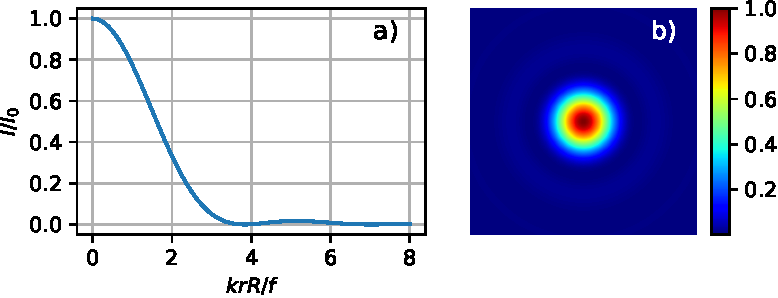
\includegraphics[width = 0.8\linewidth]{figures/AiryDisk.pdf}
    \caption{\textbf{a)} Normalized intensity of the perfect \ac{PSF} as a function of the azimuthal coordinate $r$ normalized in terms of units $f / kR$.
    \textbf{b) }2D plot of the Airy disk.  }
    \label{fig:AiryPlots}
\end{figure}

The point spread function of a circular aperture is shown in \cref{fig:AiryPlots}. 
Solving for the first zero of \cref{eq:NormalizedPSF}, and introducing the definition of numerical aperture for a compound microscope \ac{NA}: $R = \text{NA} \times f$ yields for this radius 

\begin{equation}\label{eq:Abbe}
    d_1 = 0.61 \frac{\lambdaup}{\text{NA}}
\end{equation}

This result is known as the Abbe limit or diffraction limit \cite{Hecht2002} and it is the smallest feature the imaging system can produce. 
To minimize the \ac{PSF} we can thus increase the \ac{NA} of our imaging system. In this work we will use $\text{NA} = 0.5$. 

In practice, it is not convenient to use \cref{eq:FourierBesselAperture} to fit data and it is more convenient to use a simpler function. 
A Gaussian function is commonly used, and can even fit better than \cref{eq:FourierBesselAperture} because the rings of the Airy disk are easily deformed becauese of aberrations \cite{Knottnerus2018}. 

\mbox{}\par
\begin{mdframed}
    \subsection*{Intermezzo Gaussian Beams}\label{sec:GaussianBeams}
    
    Because we will frequenty use the parameters of a Gaussian beam, we will review them here. 
    Starting from Maxwell equations, one can derive under paraxial approximation a description of the transverse electromagnetic mode (TEM\textsubscript{00}) \cite{Leeuwen2017} for the electric field $E$.
    This Gaussian beam is most conveniently written down in cylindrical coordinates $\{r,z\}$:
    
    \begin{equation}\label{eq:GaussianBeam}
    	E(r,z) = \frac{w_0}{w(z)} \exp{\left(\frac{-r^2}{w^2(z)}\right)} \exp{\left[-ikz-i\frac{kr^2}{2R(z)} - i\psi(z)\right]},
    \end{equation}
    
    with parameters
    
    \begin{equation}\label{eq:GaussianBeamParameters}
    	k = \frac{2\pi}{\lambdaup}, \quad 
    	w(z) = \sqrt{w_0 + \frac{z^2}{z_R^2}}, \quad \text{and} \quad
    	R(z) = z \left(1 + \frac{z^2}{z_R^2}\right).
    \end{equation}
    
    Respectively, the wave number in terms of the wavelength $\lambdaup$, the beam waist, the radius where the field drops $1/e$ in terms of $w(z)\equiv w_0$ and $R(z)$ is the wavefront curvature. $z_R$ is the Rayleigh range, the distance along the optical axis where the beam waist has increased a factor of $\sqrt{2}$: $w(z=z_R) = \sqrt{2}w_0$.
    Finally $\psi(z)$ is an extra phase term originating from the curvature of the wavefront known as the Gouy phase.
    We find the intensity of the Gaussian beam by taking the absolute value squared:
    
    \begin{equation}\label{eq:GaussianBeamIntensity}
    	I(r,z) = I_0 \frac{w_0^2}{w^2(z)} \exp{\left(\frac{-2r^2}{w^2(z)}\right)}
    \end{equation}
    
    A sketch of a Gaussian beam profile is given in \cref{fig:GaussianBeam}, showing the $1/e$ field radius, or $1/e^2$ intensity radius $w_0$ and the Rayleigh range $z_R$. 
    
    \vspace*{3mm}
    \centering
        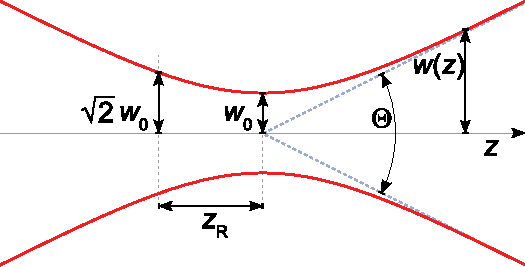
\includegraphics[width=0.5\linewidth]{figures/GaussianBeam.pdf}
        \captionof{figure}{Gaussian beam profile and some key parameters used in this work, the beam waist $w_0$ and Rayleigh range $z_R$. 
        Figure adapted from \cite{Hermans2009}.}
        \label{fig:GaussianBeam}
\end{mdframed}

Fitting this Gaussian as closesly as possible to an Airy pattern using a least-squares optimization, it can be shown that the equivalent Gaussian waist is \cite{Zhang2007}.

\begin{equation}\label{eq:GaussianAiryFit}
    w = 0.42 \frac{\lambdaup}{\text{NA}}
\end{equation}
 
If our measured waist is at this limit, the system is said to be diffraction limited, that is: the spot size is limited because of the wave character of light and not because of optical aberrations. 

\section{Optical Tweezers in Practice}\label{sec:TweezersPractice}

So to minimize the trapping volume, we need the highest possible numerical aperture. But there are more demands our lens should satisfy: the \ac{MOT} and subsequent \ac{ODT} are made in a vacuum chamber so the beam traverse a vacuum viewport. This poses additional requirements on the objective:

\begin{enumerate}
    \item Ultra-long working distance (the distance between the trap and the lens). For a single lens, this is equivalent to the focal length of course, though for a compound lens this is a bit more complicated. 
    
    \item Glass-thickness compensation. The relatively thick vacuum viewport will introduce significant (spherical) aberrations for high NA and therefore big angles. It is possible to correct for this by having an additional lens which will counteract this.
\end{enumerate}

To achieve this, we chose the G Plan Apo microscope objective from \textit{Mitutoyo}, as also used by \cite{Manuel2016,Ebadi2021}. 
This is an infinity-corrected objective, meaning light collected in its focussed is imaged at infinity (parallel beam) and an additional field lens is used to focus this image, such that the magnification is 

\begin{equation}\label{eq:InfinityMagnification}
    M = \frac{f_2}{f_1},
\end{equation}

where $f_2$ is the focal length of the field lens and $f_1$ the equivalent focal length of the objective\footnote{For a compound microscope objective, equivalent focal length means the focal length the objective would have when replaced by a single lens.}.
Relevant specifications of the objective are shown in \cref{table:MitutoyoSpecs}. 
From compound objectives, the equivalent focal length $f_1$ is defined in terms of the \ac{NA} and the back aperture radius of $R$ as $R = f_1 \text{NA} = 2$ mm. 

\begin{table}[h]
    \centering
    \caption{Key specifications of the objective from manufacterer Mitutoyo.}
    \label{table:MitutoyoSpecs}
    \begin{tabular}{l | l}
        \textbf{Specification}       & \textbf{Value} \\ \hline 
        NA                           & 0.5            \\ \hline
        Glass thickness compensation\footnote{We assume 3.5 mm of N-BK7 glass is used here, which has a slightly different refractive index than quartz for example.} & 3.5 mm         \\ \hline
        Equivalent focal length      & 4 mm           \\ \hline
        Working distance             & 15.08 mm      
    \end{tabular}
\end{table}

Because this objective was designed with visible wavelenghts in mind, it is probable that all of the lenses inside it are coated with a reflection coating that does not work well for the 800 nm regime. 
This is indeed the case, as we measured the tranmission of the objective to be just $(47 \pm 3)\%$ at 820 nm. We will therefore lose a significant of laser power. 
But this is not the only source of laser power loss: in producing the Airy pattern we assumed plane wave illumination, but in practice laser beams have Gausian shape. 
As a result, when working with a beam significantly larger than the back aperture this excess power is lost. 
Assuming the beam is aligned with the center of the aperture, the power tranmission $P/P_0$ as a function of the incident waist $w_i$ is

\begin{equation}\label{eq:fracPowerCircular}
    P/P_0 = 1 - e^{-2w_i^2/R^2}
\end{equation}

which tends to zero for very wide beams (plane waves). Clearly there is an optimum sommewhere.
To illustrate this, we will look at the other extreme case of $w_i \ll R$. 
The waist is much smaller than the aperture, according to \cref{eq:fracPowerCircular} all of the power is transmitted through the aperture.
We let the integration boundary run to infinity and using a Hankel tranform pair\footnote{$F_0(k) = \int_0^{\infty} e^{-1/2 a^2 r^2} J_0(k r)r dr = \frac{1}{a^2} e^{-\frac{k^2}{2a^2}}$} find 

\begin{equation}\label{eq:GaussianCase}
    U(r) \propto \frac{w_i^2}{2} \exp{\left(\frac{-k^2w_i^2 r^2}{2f^2}\right)}.
\end{equation}

The result is a Gaussian, but with a modified waist of $\lambdaup f / \pi w_0$.
This modified waist will go up for smaller $w_0$ (Fourier transform property). 
Clearly, this is not ideal either. 
To understand the optimum a bit better, we will define the concept of trap frequencies. 
But a priori we know the resulting potential will be something in between a Gaussian beam and an Airy pattern. 

\subsection{Tweezer Potential}

From \cref{eq:Stark} we know that the potential of the tweezer is proportional to the light intensity. 
Assuming a Gaussian tweezer beam, the potential $U$ in cylindrical coordinates will be roughly (\cref{eq:GaussianBeam,eq:GaussianBeamParameters}).

\begin{equation}\label{eq:GaussianPotential}
    U(r,z)=\frac{-U_{0}}{1+z^{2} / z_{R}^{2}} \exp \left(\frac{-2 r^{2}}{w_{0}^{2}\left(1+z^{2} / z_{R}^{2}\right)}\right)
\end{equation}

\cref{eq:GaussianPotential} is plotted in \cref{fig:GaussianPotential} for normalized radial coordinate $r/w_0$ as well as longitudinal coordinate $z_R$. 
This is not to scale: the Rayleigh range $z_R$ is typically bigger than the waist $w_0$.
Assuming a Gaussian is justified because near the center, an Airy disk and Gaussian beam are nearly identical.
We are interested in potentials much deeper than the temperature of the atoms, such that the atoms will mostly occupy the bottom of the tweezer. 
Taylor expanding \cref{eq:GaussianPotential} around $(r,z)=(0,0)$ to second order yields 

\begin{figure}
    \centering
    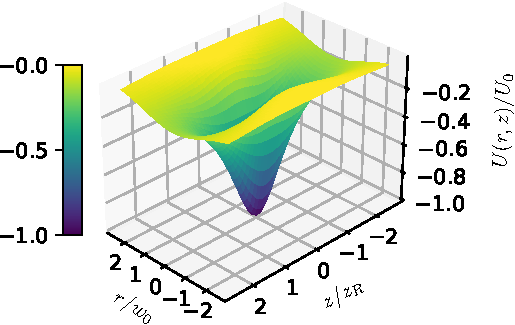
\includegraphics[width=.56\linewidth]{figures/GaussianPotential.pdf}
    \caption{Normalized potential from a Gaussian intensity shape. The independent coordinates are the normalized cylindrical coordiantes $r/w_0$ and $z/z_R$.}
    \label{fig:GaussianPotential}
\end{figure}

\begin{equation}\label{eq:ApproximateGaussianPotential}
    U(r,z) \sim -U_0 - 2U_0 \frac{r^2}{w_0^2} - 2U_0 \frac{z^2}{z_R^2}
\end{equation}

For this harmonic potential, one can compute the harmonic oscillation frequencies 

\begin{equation}\label{eq:TrapFrequencies}
    \omega_r = 2\left(\frac{U_0}{m w_0^2}\right)^{1/2}, \quad
    \omega_z= \left(\frac{2 U_0}{m z_R^2}\right)^{1/2}
\end{equation}

Because $z_R > w_0$, the longitudinal oscillation frequency is lower than the radial frequency. 
Trap frequencies are a nice property to optimize, because from the definition, higher trap frequencies translate to deeper as well as sharper tweezers. 
\cite{Madjarov2021} optimized \cref{eq:TrapFrequencies} for the $w_i/R$ ratio and found an optimum around $w_i\sim R$, which we will use in this work\footnote{Because trap frequencies can be probed exprimentally, they can be used to perform post-corrections on tweezer arrays as well as shown by \cite{Ebadi2021}.}.

\section{Measuring the Tweezer potential}

We would like to measure tweezer potential made by our microscope objective. 
We could use time symmetry and look at the reverse direction: using the objective to look at a pinhole, retrieving its \acf{PSF} \cite{Knottnerus2018,Sortais2007}
However, using this method the objective will produce a plane wave, when we know that in practice we do not send a plane wave to the objective as discussed in \cref{sec:TweezersPractice}
function. 

Instead, we used another microscope objective, to look into produced tweezer potential by the \textit{Mitutoyo}. 
In doing this, the tweezer potential will be convolved with the \ac{PSF} of the second microscope objective\cite{Baumgaertner2017}.
Therefore we used a second microscope objective\footnote{Newport M-60X 0.85 NA objective.} with significantly higher \ac{NA}, minimizing this effect. 

\subsection{Optical Setup}

In the actual machine, we use an optically contacted glass cell as our vacuum chamber. Because no objective exists that has significantly higher NA than 0.5 as well as ultra-long working distance, we can not look into the glass cell using this method. Therefore, we use a piece of glass with the same thickness and material (quartz glass, $d = 4.0$) mm to imitate the glass cell. The second objective will produce an image onto a linear CCD camera\footnote{Point Grey FLEA2 FL2-08S2M.}. Because alignment of the Mitutoyo objective with the incident beam, as well as alignment of the two objectives with respect to each other is crucial, both objectives are mounted on piezo-controlled 5 axis translation stages. 
This is drawn in the lower-right corner of \cref{fig:TiSandSLMsetup}.

On top we show the laser source used.
This laser is positioned on a separate table and its output is brought to the main table using a \ac{PM} optical fiber. 
The laser source is a \ac{Ti:S} ring laser\footnote{\textit{Coherent} 899-21 ring laser} (linewidth $\sim 1$ Mhz, output power max. $\sim 1$ W.). 
The crystal is pumped using a pump laser\footnote{\textit{Coherent} Verdi V18} (18W power, 532 nm). 
The \ac{Ti:S} is eaily tunable in wavelength over a wide range. For Sr 813 will be used, but for the experiments for Rb we used 820 nm. 
In between the laser source and the objective, there is a \ac{SLM}. But the SLM has its own \cref{ch:arrays}, so will not get into that now. 
In day to day tuning of the mirrors inside the Ti:S ring laser, the output angle and therefore the fiber coupling efficiency is slightly changed. 
To ease the coupling, we run a coax cable from a power meter on the main table to a multimeter on the Ti:S table. 

\begin{figure}
    \centering
    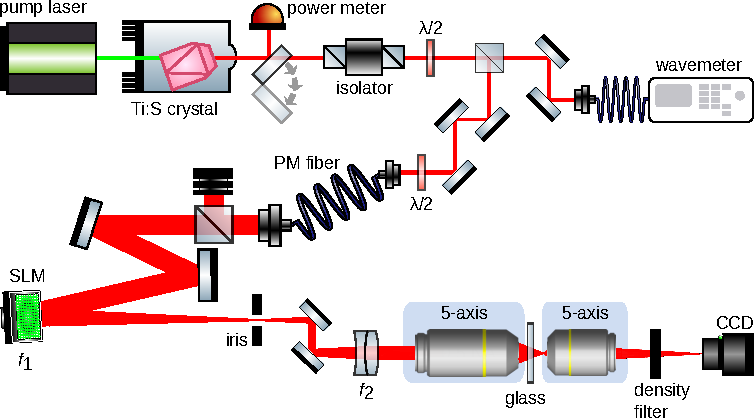
\includegraphics[width=0.8\linewidth]{figures/TiSandSLM.pdf}
    \caption{Optical setup for making an optical tweezer and imaging this tweezer onto a CCD camera. 
    Laser source decribed int the text and \ac{SLM} more thoroughly in \cref{ch:arrays}.
    The titanium sapphire laser is positioned on a separate table. 
    All cubes are polarizing.}
    \label{fig:TiSandSLMsetup}
\end{figure}

\subsection{Calibration Imaging System}

The 60X magnification of the 0.85 NA objective is only specified when used in a microscope with standard tube length distance, because it is finite conjugate corrected.
Because our CCD is not exactly at the distance where normally the eyepiece of the microscope would be, we have to calibrate its magnification.
We do this using a high resolution target\footnote{Edmund Optics high resolution microscope target.}.

This target is illuminated with incoherent light from a \ac{LED} because we noted that using a coherent source from a laser caused too much interference from the different lines. We neglect the slightly different focus point from the Newport objective for our laser frequency compared to white light. 

\begin{figure}
    \centering
    \includegraphics[width = 0.45\linewidth]{figures/linespacing.pdf}
    \caption{Image from the resolution target illuminated showing lines spaced by 45 lines per mm.}
    \label{fig:resolutionTarget}
\end{figure}

To detect the edges in \cref{fig:resolutionTarget}, we use an edge detection algorithm script that averages over all vertical pixels, blurs using a Gaussian to surpress noise and computes the derivative. 
When the derivative surpasses a set threshhold we define it as an edge.
The magnification was found to be $(50.3\pm0.5)$X.
This is smaller than the specified 60X, which we attribute to an incorrect tube length distance. 

\section{Tweezer Images: Radial}

An image of the CCD camera is shown in \cref{fig:SingleSpotZoomed}. 
There seems to be a small tilt aberration present as the side ring is more clearly visible on the right side. 
We found aberrations of this magnitude almost impossible to get rid of, as it could originate from anywhere between the input beam and the camera.

In \cref{fig:AzimuthalAverage} we have integrated the intensity in rings around the maximum with a width of 1 pixel, effectively computing an azimuthal average. 
This result is compared against the \ac{PSF} of the objective (\cref{eq:NormalizedPSF}), as well as the result from scalar diffraction theory using a Gaussian input beam equal to the aperture $w_i \sim R$, which was obtained by computing \cref{eq:FourierBesselAperture} for a sample of radial coordinates $r$. 
\begin{figure}
\centering
    \centering
	\begin{subfigure}{.49\textwidth}
		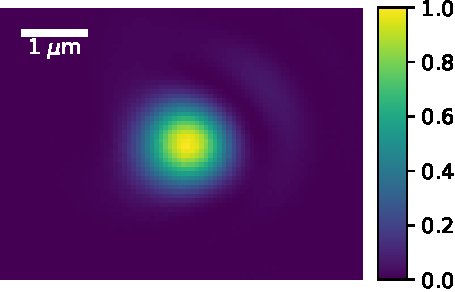
\includegraphics[height=4.9cm]{figures/SingleSpotZoomed.pdf}
		\caption{}
		\label{fig:SingleSpotZoomed}
	\end{subfigure}
	\begin{subfigure}{.49\textwidth}
		\centering
		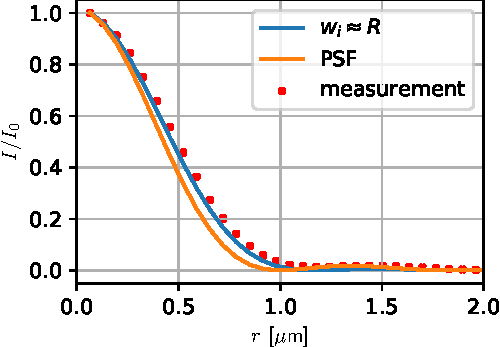
\includegraphics[height=4.9cm]{figures/AzimuthalAverage.pdf}
		\caption{}
		\label{fig:AzimuthalAverage}
	\end{subfigure}
	\caption{\textbf{a)} Tweezer as imaged by the second objective onto the CCD camera. 
	\textbf{ b)} Azimuthal average (red) plotted against the \ac{PSF}, \cref{eq:NormalizedPSF} of the objective as well as the Gaussian input beam formula \cref{eq:FourierBesselAperture}.}
	\label{fig:2Dresults}
\end{figure}

So, if a Gaussian input beam used, the resulting spot will be slightly broader.
Additionally, the rings of the Airy disk will be slightly surpressed, this effect is known as Gaussian apodization.
This plot is convenient for showing the general behavior, but is not accurate enough to extract data like the waist. 
For example: in this binning method, distance to the center pixel are calculated, but the center could be anywhere on this pixel. 
Therefore we also perform a two-dimensional Gaussian fit using \cref{eq:2DGaussian}.

\begin{equation}\label{eq:2DGaussian}
    \frac{G(x,y)}{G_0} =  
    \exp{\left[ -\frac{(x-x_0)^2}{2\sigma_x^2}\right]}
    \exp{\left[ -\frac{(y-x_0)^2}{2\sigma_y^2}\right]}
\end{equation}

The result of this fit is shown in \cref{fig:3DFitShowing}. 
Cleary, the obtained tweezer potential fits very well to a Gaussian, which justifies the assumption of using a Gaussian approximation to estimate the trap frequencies (\cref{eq:GaussianPotential}. 
This is confirmed by the coefficient of determination $R^2 > 0.99$.

\begin{figure}
    \centering
    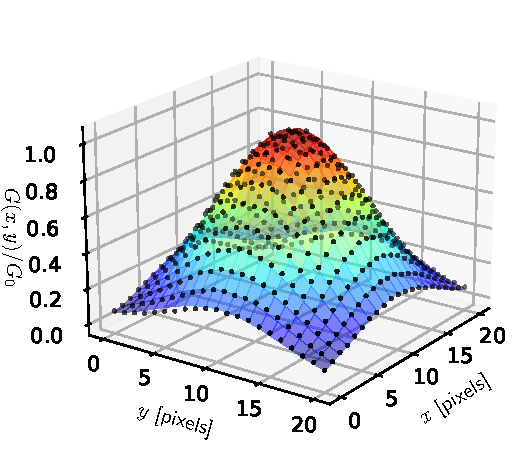
\includegraphics[width=0.5\linewidth]{figures/3DSpotFitGaussian.pdf}
    \caption{Plot showing quality of the Gaussian fit. $R^2 > 0.99$}
    \label{fig:3DFitShowing}
\end{figure}

Assuming the $\sigma_x \sim \sigma_y$ which should be the case for a circlar aperture, we find the waist as $w_0 = \sigma_x + \sigma_y = (0.80 \pm 0.03)$ $\mu$m, where the error originates mainly from the calibration of the magnification. 
We fitted a region of interest around the spot maximum of 10 x 10 pixels. 
Comparing to the theory result, for $\lambdaup = 820$ nm and $\text{NA} = 0.5$ (\cref{eq:GaussianAiryFit}) yields $w_0 = 0.689$ $\mu$m. 
But this result unachievale because of $w_i \sim R$ used. 
We know that as a result of this, the waist should be $\approx$9\% larger \cite{Sortais2007} which was confirmed by \cref{eq:FourierBesselAperture}, yielding $w_0 = 0.751$ nm. 
So our tweezer is about 6\% broader than the theoretical minimum, which is to be expected because of aberrations. 
We did apply some aberration correction, which is mainly described in the next section \cref{sec:Tweezer3D}.
The result shown is after this aberration correction, though this this not significantly improve the result. 
We did note an improvement mainly for the axial direction which the next section is about. 

\section{Tweezer: Axial Direction}\label{sec:Tweezer3D}

For the volume of the tweezer not only the radial direction is important, but the axial (longitudinal) direction as well. 
The relevevant quantity here is the Rayleigh range (see \cref{fig:GaussianBeam}).
For the radial images shown in \cref{fig:2Dresults} we were intially surprised that the results was already pretty good even before aberration correction, because we know for example that the optical thickness of the glass cell (and the quartz plate that replaces the glass cell, \cref{fig:TiSandSLMsetup} is about 0.5 mm too thick: the objective is designed for 3.5 mm of N-BK7 (refractive inded $n = 1.51$, $nd = 5.3$ mm) whereas the cell is 4.0 mm of quartz glass ($n = 1.44$, $nd = 5.8$ mm). 
This might seem insignicant, but because of the high \ac{NA} and consequently large angles under which the light traverses the glass, it is possible the outer (marginal) rays will focus at at a slightly different point than the inner (paraxial) rays. 
To study the axial direction, we scan the Mitutoyo objective along the optical ($z$) axis and record an image of the tweezer. 
In the end, all images are stiched together to make a single image that would give an idea of a sideview of the tweezer.
This is done in figure.
Also plotted in this figure is the result from diffraction theory. 
To calibrate the amount of translation we calibrated the step size of the motor.


\subsection{Picomotor Attenuator Calibration}

Piezo-controlled attenuaters are very good at producing minisclule ($<30$ mm) step sizes. The step size is also extremely constant, making them ideal for axials scans like this.
The stage we used is 8081-M 5-axis motorized tilt aligner from Newport. 
Because of the 5 degrees of freedom, it can accurately align the two objectives with each other. 
To drive this stage, we used a set of Newport 8742 controllers in daisy-chain configuration: both can drive 4 motors so we have 2 of them to address all 5 motors.
For scanning the axial direction of the tweezer we only use one of the 5 motors inthe stage. 


However, to know the exact step size calibration is needed because the step size is dependent on the torque applied, which depends on the direction of travel as well as whether the motor has to counter gravity, etc.
In order to do this, we repeatedly measured the available translation range of some $\sim$ 3mm, recording the amount of steps this takes as well as the amount moved using a caliper. 
We found a step calibration of $10.6 \pm 0.05$ $\mu$m/step, which was used to translate amount of steps to distances. 











\chapter{Tweezer Arrays}\label{ch:arrays}
    \section{Introduction}

For a quantum computer, multiple qubits are needed that are capable of interacting with each other. 
Thus, we need to make an array of the tweezers described in \cref{ch:tweezer}, spaced from each other in the order of micrometers. 
This can be done by sending several laser beams to the objective, each under slightly different angles. 
Experimentally, this could be realized using an \ac{AOD}: a device that diffracts light off of a sound wave in a crystal, where the degree of diffraction is controlled by a \ac{RF} signal. 
By using 2 AODs in an orthogonal configuration, each supplied by a superposition of RF signals (see \cref{fig:CrossAOD}), 2D arrays of optical tweezer were successfully realized \cite{Manuel2016}. 

Nevertheless, one drawback of this method is that there is little flexibility in varying the individual laser spot intensities because of the crossed configuration.
Therefore, it was proposed to use holography methods for producing arrays of optical tweezers instead \cite{Bergamini2004}, making use of a \acf{SLM}.
Using an SLM for tweezer arrays has the advantage that it is possible to dynamically adapt the hologram, correcting for variation within trap depths of the array \cite{Nogrette2014}. 
At the same time, SLMs also allow for the correction of optical aberrations introduced by the optics in the setup \cite{Bijnen2015}.
Lastly, using the holographic method, it is even possible to make 3D arrays of tweezers \cite{DiLeonardo2007,Barredo2016}, though we will limit ourselves to 2D arrays in this work.

In the following section \ref{sec:SLM} we will introduce the working principle of the SLM, as well as the algorithm used to compute the holograms needed.
Next, in \cref{sec:SLMoperatoin} we elaborate how we used the SLM in the practice. 
Finally, in \cref{sec:ArraysResults} we present the measured spot arrays.



\section{The Spatial Light Modulator}\label{sec:SLM}

A spatial light modulator is in essence a device that can imprint a computer generated hologram onto a beam of light, allowing the spatial shaping of this light.
Different types of SLMs can manipulate properties of light like amplitude, phase and polarization.
In this work a phase-only reflective SLM was used, which as the name suggests can only control local phase of the incoming light field.
The use of phase-only SLMs has been extensively covered in our group by, for example by \cite{Bijnen2015,Dijk2012,Bijnen2013}. 

The modulating works by deploying a pixel array, where each pixel houses a liquid birifringent crystal.
By applying a voltage (electric field) over the pixel, the orientation of the liquid crystal molecules change, changing their effective refractive index.
This principle is sketched in \cref{fig:LCoS}.
Because of crystals are birifringent they posses refractive indices among perpendicular axes, commonly referred to as the ordinary and extraordinary refractive indices respectively ($n_o$ and $n_e$). 
If the light travels a distance $t$ in a crystal unit of the SLM, the phase retardation will be $\phi_o = k t n_o$ and $\phi_e(V) = k t n_e(V)$ respectively (only the extraordinary axis can be modulated), such that the phase retarder can be represented by the Jones matrix \cite{Guzman2017}

\begin{equation}\label{eq:JonesMatrix}
    M = e^{i \phi_0} 
    \begin{pmatrix}
        e^{i(\phi_e-\phi_o)} & 0\\
        0 & 1
    \end{pmatrix}.
\end{equation}
Thus the phase retardance $\phi$ as a function of the applied voltage $V$ is \cite{Guzman2017}, using the birifringence parameter $\Delta n= n_e-n_o$

\begin{equation}\label{eq:ElectroOpticResponse}
    \phi(V) = k t(n_e(V) - n_0) t = \frac{2\pi}{\lambdaup}t \Delta n(V).
\end{equation}
To obtain voltage control over each individual pixel, the display is manufactured on a layer of silicon, making use of various semiconductor manufacturing technologies.
As a result of diffraction from the various pixels, one can create arbitrary intensity patterns in in the focal plane of a lens.
This concept is sketched in \cref{fig:SLMLens} and further explained in the next section.


\begin{figure}
	\begin{subfigure}{.39\textwidth}
		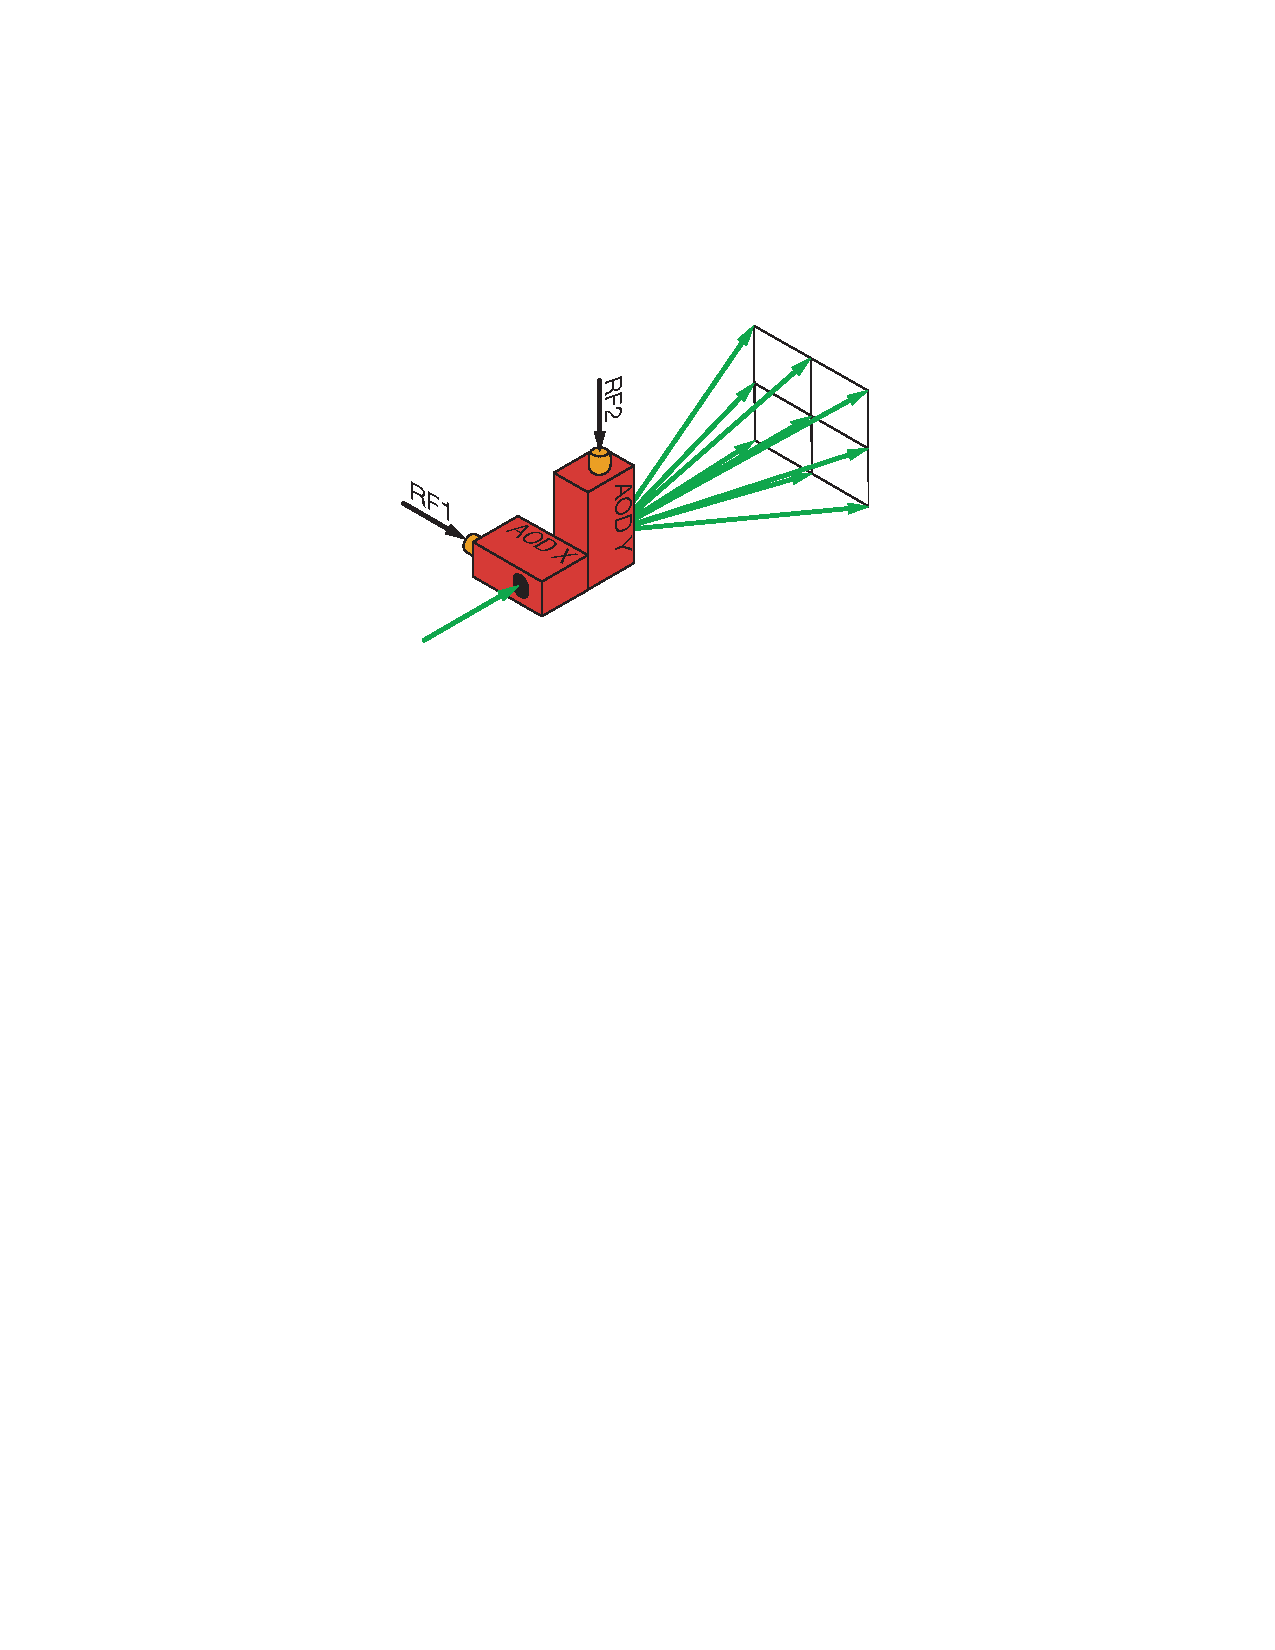
\includegraphics[height=4.25cm]{figures/crossAOD.pdf}
		\caption{}
		\label{fig:CrossAOD}
	\end{subfigure}
	\hfill
	\begin{subfigure}{.59\textwidth}
		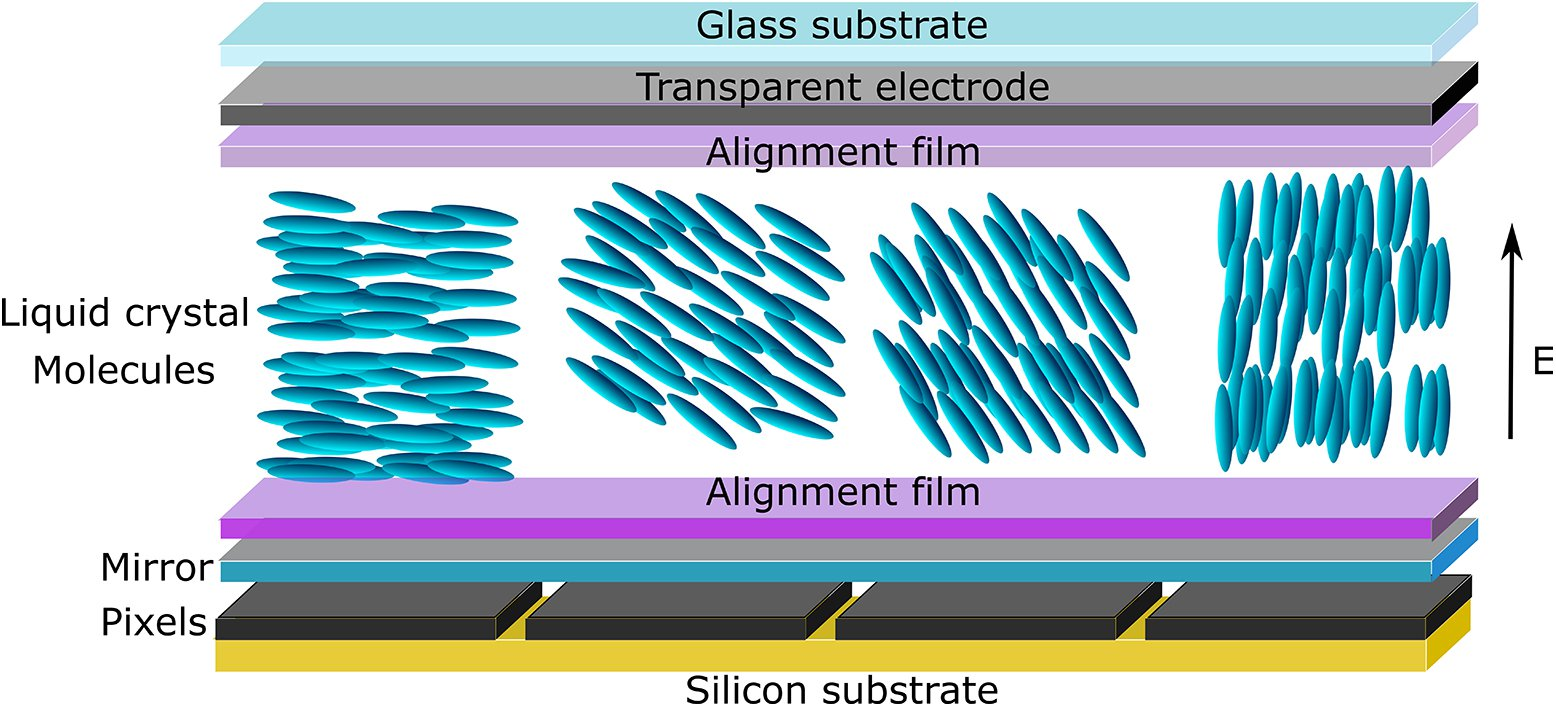
\includegraphics[height=4.25cm]{figures/LCoS.png}
		\caption{}
		\label{fig:LCoS}
	\end{subfigure}
	\caption{\textsf{\textbf{a)}} Two \ac{AOD}s in crossed configuration, used to make a 2D spot array. Figure from \cite{Cooper2018}. 
	\textsf{\textbf{b)}} The orientation of the liquid crystal cells changing as a function of the applied electric field \textit{E}. 
	Figure from \cite{Guzman2017}.}
\end{figure}


\subsection{Diffraction for Spot Arrays}\label{sec:PropagationDerivation}

We will now delve deeper in the diffraction from the SLM hologram, limiting ourselves to producing spot arrays.
First consider plane of the SLM, denoted in \cref{fig:SLMLens} by the Cartesian coordinates $(x',y',z=0)$. 
If we label the pixels of the SLM with the letter $j$, the phase retardance of this pixel is thus $\phi_j(x'_j,y'_j)$.
Now, consider a laser with intensity distribution $|E_i(x',y')|^2$ reflecting off of the SLM: it will pick up a phase factor such that after the SLM, the field is described as $E_i e^{i\phi(x',y')}$, as shown in \cref{fig:SLMLens}. 
The light field will interfere with itself, until at infinity (or approximately in the focal (Fourier) plane $z'=f$, $z=0$ of a lens) the distribution evolves to $|E_f(x,y,z)|^2$, where $(x,y,z)$ are Cartesian coordinates with the origin in the focus point of the lens as denoted in \cref{fig:SLMLens}.

To see how this works, consider the focal plane or Fourier plane of a lens after the SLM\footnote{In reality, the distance between the SLM and the microscope objective is not the focal length $f$ of the objective, but this will lead to an additional phase factor which can be neglected in practice \cite{Bijnen2013}.}.
In the Fourier plane, the spots in the array will be labeled as $m$, which in general have coordinates $(x_m, y_m, z_m)$ in the Fourier plane, see \cref{fig:SLMgeometry}.
As result of traveling from the pixel $j$ to the trap $m$, under paraxial approximation it can be derived the light field will experience a phase shift $\Delta_j^m$ \cite{DiLeonardo2007}

\begin{figure}
	\centering
	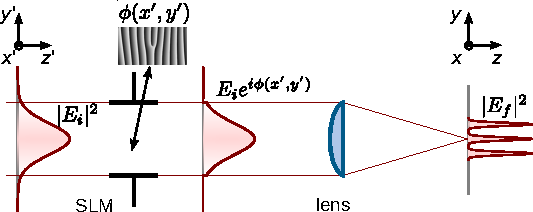
\includegraphics[width = 13cm]{figures/SLMfigure.pdf}
	\caption{Field with intensity distribution $|E_i|^2$ reflects off of the   rectangular SLM, which due to its finite size acts as an aperture in the short-axis direction.
	Also the SLM imprints a phase mask $e^{i\phi(x',y')}$ onto the laser.
	The lens (microscope objective) makes the resulting spot array $|E_f|^2$ in its focal plane.
	Shown on top: two Cartesian coordinate systems in the SLM and focal plane respectively. 
	Figure adapted from \cite{Labuhn2016}.}
	\label{fig:SLMLens}
\end{figure}

\begin{equation}\label{eq:PropagationPhase}
    \Delta_j^m = 
    \frac{2\pi z_m}{\lambdaup f^2} ({x'}_{j}^{2} + {y'}_{j}^{2}) 
    + \frac{2\pi}{\lambdaup f}(x'_j x_m + y'_j y_m).
\end{equation}
The SLM imprints a phase $\phi(x',y') = \phi_j$, leading to a complex SLM plane for pixel $j$ of

\begin{equation}\label{eq:SLMassumption}
    E_j(x',y') = E_j e^{i \phi_j}.
\end{equation}
In the Fourier plane, the contributions for the different pixels will interfere with each other.
We can find the complex light field $V_m$ (for this section, we will denote the complex light field in the Fourier plane as $V$ similar to \cite{DiLeonardo2007}) for trap $m$ by summing over $N$ pixels $j$ using \cref{eq:PropagationPhase,eq:SLMassumption} \cite{Leseleuc2018}

\begin{equation}\label{eq:DiffractionFormula}
    V_m = e^{i k \left(2 f + z_m\right)}
    \frac{d^2}{i \lambdaup f} \sum_{j=1}^N E_j e^{i(\phi_j - \Delta_j^m)},
\end{equation}
which is essentially using a discrete version of the Fresnel diffraction integral, where $d$ is the pixel pitch of the SLM. 
In \cref{eq:DiffractionFormula}, we can assume uniform illumination of the SLM such that the amplitude is the same everywhere on the SLM or $|E_i| = 1$.
This assumption cannot possibly be valid: we illuminate the SLM with a Gaussian beam from an optical fiber.
However, as will become clear in a moment, the input intensity on the SLM will have no influence on the intensities in the focal plane and this assumption can in fact be used without loss of generality.
In addition, we are really only interested in the intensity $I_m =|V|^2$ of each spot, not the phase.
Omitting the pre-factors in \cref{eq:DiffractionFormula} thus yields

\begin{equation}\label{eq:Vm}
    V_m \propto \sum_{j} e^{i(\phi_j - \Delta_j^m)}.
\end{equation}
This equation gives the complex field amplitude for spot $m$, given a hologram $\phi_j$.
While \cref{eq:Vm} can be used to compute intensities of 3D spot arrays, an instructive example is setting $z=0$ first \cite{DiLeonardo2007}, for which the quadratic term of \cref{eq:PropagationPhase} disappears.
Substituting the latter term of \cref{eq:PropagationPhase} in \cref{eq:Vm} yields a 2D array of spots with amplitudes 

\begin{equation}\label{eq:2Dcase}
    V_m \propto \sum_j e^{i\phi_j} \exp{\left(
    - i 2\pi \left[
    \frac{x_m}{\lambdaup f} x_j + \frac{y_m}{\lambdaup f} y_j
    \right]
    \right)},
\end{equation}
Which is the 2D \ac{DFT} of $e^{i\phi}$ evaluated at spatial frequencies $x_m/\lambdaup f$ and $y_m/\lambdaup f$ in $x$ and $y$ respectively \cite{Bijnen2015,DiLeonardo2007}, similar to \cref{eq:FraunhoferDiffractionIntegral}.
Using \cref{eq:2Dcase} has the advantage that the DFT is much faster to evaluate than the general case of the diffraction formula \cref{eq:Vm} using the \ac{FFT}.
In this work, we only use 2D arrays and could in principle use \cref{eq:2Dcase} to speed up calculations.
Because we only computed a small number of holograms, we simply used \cref{eq:Vm}.

\subsection{Computing the Hologram}\label{sec:GSW}

\Cref{eq:Vm} gives the amplitudes of an array of spots given an array of phases $\phi_j$, but we are interested in the reverse problem: what is the hologram $\phi_j$ to be applied, such that we get the spot array of intensities $|V_m|^2$? 
As the equations describing light propagation are time-symmetric, this phase will be the result of $M$ coherent light sources radiating with $w_m e^{i \theta_m}$, picking up a propagation phase described by \cref{eq:PropagationPhase}, leading to a complex amplitude in the \ac{SLM} plane of \cite{DiLeonardo2007,Leseleuc2018}

\begin{equation}\label{eq:InterferencePattern}
    E_j (x',y') = \sum_m w_m \exp{
    i\left(\Delta_j^m + \theta_j\right)
    }.
\end{equation}
But producing the the light field in \cref{eq:InterferencePattern} requires doing phase as well as amplitude modulation, which is not possible: the SLM can only do phase modulation.
So in this step in the algorithm, we take the argument of  \cref{eq:InterferencePattern} yielding the following hologram

\begin{equation}\label{eq:Argument}
    \phi_j = \text{arg}\left\{
     \sum_m w_m \exp{
    i\left(\Delta_j^m + \theta_j\right)
    }
    \right\}.
\end{equation}
But the lack of amplitude modulation leads to a loss of information, and the hologram produced by \cref{eq:Argument} will not produce the result we seek.
The solution to this problem was solved by \cite{Gerschberg1972}, who pioneered the \ac{IFTA} algorithm or Gerschberg-Saxton algorithm.
The core idea of the algorithm is to virtually propagate light between SLM and focal planes, using (inverse) Fourier transforms like \cref{eq:2Dcase}.
In each propagation step, the hologram in the SLM plane and the computed pattern in the Fourier plane are updated in an iterative fashion, until a solution (the desired pattern and the corresponding hologram) are obtained.
For a more detailed description of an implementation of IFTA algorithms the reader is referred to \cite{Bijnen2015,Bijnen2013}.
A key advantage of using these kind of algorithms is that \cref{eq:Vm}: each pixel contributes to individual spot.
As a result, using this algorithm, no knowledge about the laser input field is needed, which can be hard to determine exactly in practice.

For 3D spot arrays, Fourier transforms cannot be used, and the algorithm was extended using \cref{eq:Vm,eq:Argument} by \cite{DiLeonardo2007}. 
This algorithm is called the \ac{GSW} algorithm, which is sketched in \cref{fig:GSWalgorithm}.

\begin{figure}
	\centering
	\begin{subfigure}{.56\textwidth}
		\centering
		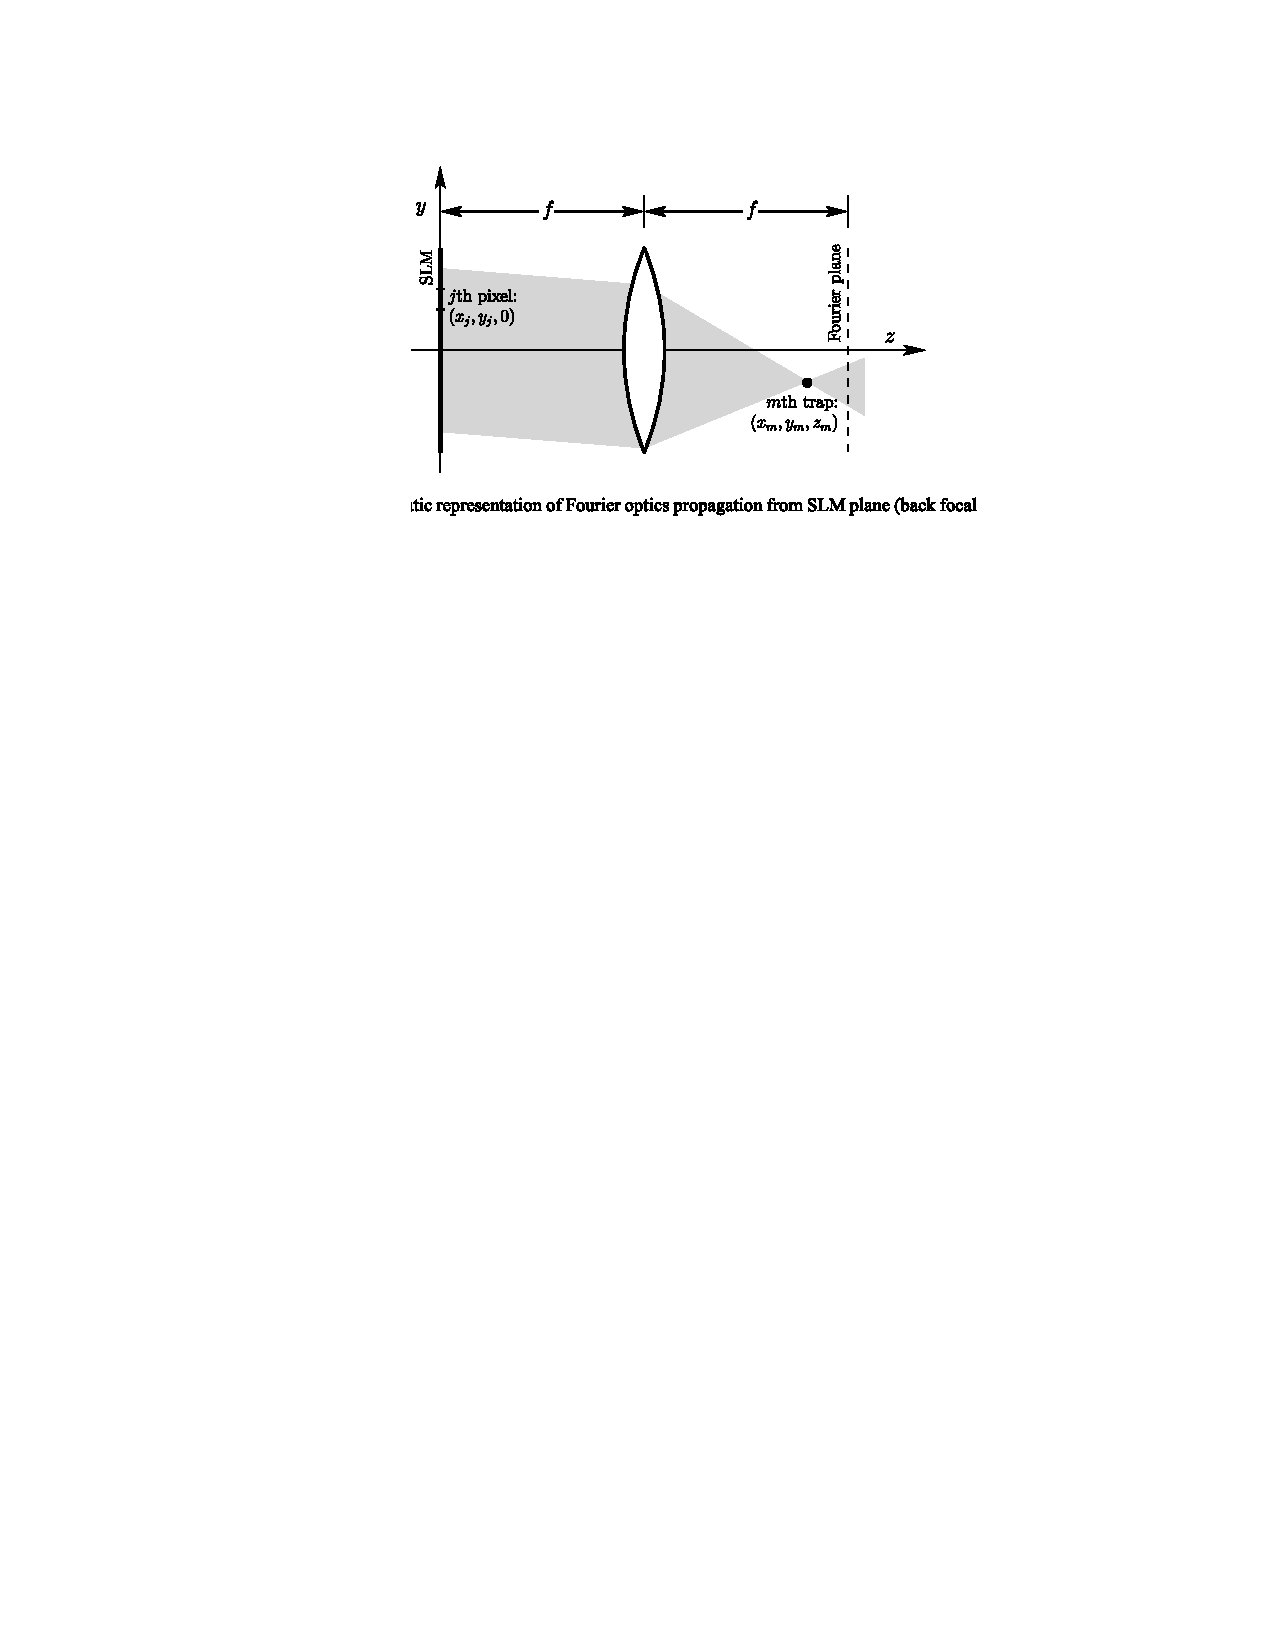
\includegraphics[height=5.3cm]{figures/SLMgeometry.pdf}
		\caption{}
		\label{fig:SLMgeometry}
	\end{subfigure}
	\begin{subfigure}{.43\textwidth}
		\centering
		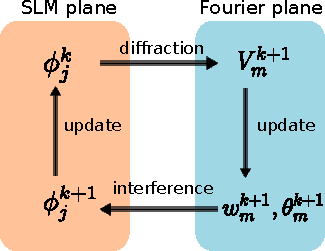
\includegraphics[height=5.3cm]{figures/WeightedGerschbergSaxton.pdf}
		\caption{}
		\label{fig:GSWalgorithm}
	\end{subfigure}
	\caption{\textsf{\textbf{a)}}SLM plane with phases $\phi_j(x,',y',z=0)$ for pixel $j$, as well as the focal plane or Fourier plane with trap coordinates for trap $m$ of $(x_m,y_m,z_m)$. 
		Figure from \cite{DiLeonardo2007}. 
		\textsf{\textbf{b)}} The \ac{GSW} algorithm visualized.
		The light field is virtually propagated between the SLM and focal planes using \cref{eq:Vm,eq:Argument}, continuously updating the weight factors $w_m^k$ as well as the hologram $\phi_m^k$.}
	\label{fig:GerschbergSaxton}
\end{figure}

\subsubsection*{The GSW Algorithm}

\begin{itemize}
    \item Starting with hologram $\phi_j^k$ diffraction equation \cref{eq:Vm} is used to compute the complex amplitudes of the spot array $V_m^{k+1}$. 
    
    \item From the amplitudes, the new weight factors $w_m^k$ and phases $\theta_m^k$ are computed, which are used to compute a new hologram using the interference equation \cref{eq:Argument}.
    
    \item The iteration counter $k$ is increased, the hologram is updated and the steps above are repeated.
\end{itemize}
The algorithm starts with a hologram hologram, $\phi_j^{k=0}$ is computed by using \cref{eq:Argument} for an array of traps of uniform intensities $w_m^{k=0} = 1$ and random phases $\theta_m^{k=0}$.
After each iteration, the diffraction efficiency $e$ (the real part of the complex interference pattern) and the uniformity $u$ of the array $V_m$ should increase until convergence, yielding a set of target amplitudes $V_m$ as well as a hologram $\phi_j$ that produces this set of amplitudes.
The definitions of the diffraction efficiency $e$ and uniformity $u$ are 

\begin{equation}\label{eq:EfficiencyUniformity}
    e = \frac{1}{M}\sum_m I_m = \frac{1}{M}\sum_m |V_m|^2, 
    \quad 
    u = 1-\frac{\text{max}(I_m)-\text{min}(I_m)}{\text{max}(I_m)+\text{min}(I_m)},
\end{equation}
and are evaluated after each iteration $k$. 
The algorithm stops if the user-defined minimum criteria for diffraction efficiency or uniformity are met.

\subsubsection*{Implementation}

The algorithm was implemented in Python by Ivo Knottnerus as part of his PhD research.
Because the SLM has $\sim 2$ million pixels, converting to and from the SLM plane, so performing equations \cref{eq:Vm,eq:Argument} can be time consuming depending on the desired pattern.
Therefore, these computations are performed on a graphics card using the \textit{PyOpenCL} library. 
After a couple tens of iteration steps, we typically see the diffraction efficiency convergence to $e \sim 0.93$.
The theoretically computed uniformity will continue to increase indefinitely, but is typically already on the order $u \sim 0.999$ after $\sim 10^2$ iterations.
A typical hologram using the algorithm is shown in \ref{fig:SLMphase}a as well as \ref{fig:HologramPattern}.


\section{Operating the SLM}\label{sec:SLMoperatoin}

Because the SLM used previously in our group suffered from amplitude modulation \cite{Bijnen2015,Dijk2012}, an unwanted effect, we purchased a newer model SLM. Specifically, the Meadowlark E-series 1920 x 1200 SLM.
A few specifications of the device are presented in \cref{table:SLMspecs}.
In the next section, we will elaborate upon some other practical considerations that have to be taken into account in operating the SLM.

\begin{table}[h]
    \centering
    \caption{Key specifications of the Meadowlark SLM.}
    \label{table:SLMspecs}
    \begin{tabular}{l | l}
        \textbf{Specification}              & \textbf{Value}        \\ \hline 
        Array size                          & 15.4 x 9.6 mm         \\ \hline
        Resolution                          & 1920 x 1200 pixels    \\ \hline
        Bit depth                           & 8 bit                 \\ \hline
        Diffraction efficiency (785 nm)  & 76-79\%   
    \end{tabular}
\end{table}


\subsection{Electro-Optical Response}

The refractive index $\Delta n(V)$ and therefore the light retardation $\phi(V)$ of \cref{eq:ElectroOpticResponse} are not necessarily linear as a function of the applied voltage.
Thus it is needed to calibrate the electro-optic response of the \ac{SLM}, which equates to measuring the retardation $\phi$ as a function of the applied voltage $V$. 
This calibration serves two purposes:

\begin{enumerate}
    \itemsep=0pt
    
    \item Ensure the minimum to the maximum phase retardation corresponds to a $2\pi$ (one wave) phase retardation.
    
    \item Linearize this electro-optical response curve. 
\end{enumerate}
The calibration has to be performed because each individual SLM has a slightly different electro-optical response. 
Furthermore, it is wavelength specific, which is why we performed it for the wavelength relevant for Rb experiments at 820 nm. 
Measuring the electro-optical response directly is impossible because the light field oscillates with frequencies in the THz regime.
There are a variety of methods to measure it indirectly for a phase-only \ac{SLM}, however \cite{Li2019}.
We chose the diffractive calibration method, originally proposed by \cite{Zhang1994}.

The method works by applying a variety of Ronchi gratings onto the SLM, see \cref{fig:LUTCalibrationSetup}.
This is a pattern consisting of $M$ periods $w=8$ pixels in the horizontal direction and a vertical height $H$ of alternating gray values $L_1$ and $L_2$.
Gray values are 8 bit number representing the degree of modulation where 0 (white) mean no voltage while 255 (black) is maximum voltage. 
Assuming amplitude modulation between different gray levels is negligible (a fair assumption for phase-only SLMs), the electric field just after the SLM is proportional to the phase transmittance given by summing over the gratings $m$ \cite{Zhang1994}

\begin{figure}
	\begin{subfigure}{.49\linewidth}
		\flushleft
		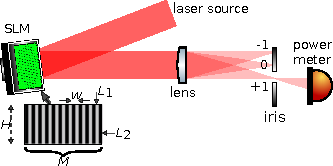
\includegraphics[height=5.1cm]{figures/LUTcalibrationSetup.pdf}
		\caption{}
		\label{fig:LUTCalibrationSetup}
	\end{subfigure}
	\hfill
	\begin{subfigure}{.49\linewidth}
		\flushright
		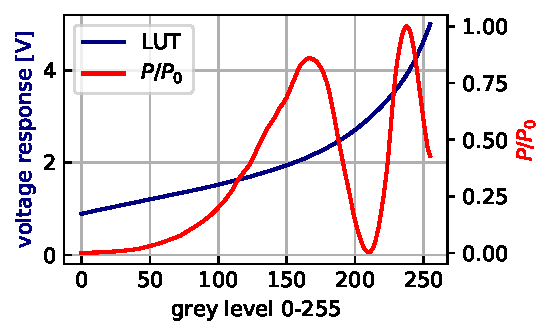
\includegraphics[height=5.1cm]{figures/LUTplot.pdf}
		\caption{}
		\label{fig:LUTcalibration}
	\end{subfigure}
	\caption{\textsf{\textbf{a)}} Ronchi grating on the SLM with gray values $L_1$ and $L_2$. 
	The diffraction order are separated using a $f=400$ mm lens. 
	Other diffraction orders than $+1$ are blocked using an iris. 
	\textsf{\textbf{b)}} Normalized power in the first order as a (\textcolor{red}{red}) and the fitted voltage response (\textcolor{blue}{blue}) as a function of the applied gray level $L_1 \in (0-255)$.}
\end{figure}

\begin{equation}\label{eq:FieldAfterSLM}
    f(x',y') = \sum_{m=0}^{M-1} \left\{
    \operatorname{rect}\left(\frac{x'-m w - w/4}{w/2}\right) + e^{i \phi(L)} \operatorname{rect}\left(\frac{x'- m w - 3 w/4}{w/2}\right)
    \right\},
\end{equation}
where $\operatorname{rect}(\cdot)$ is the rectangular function. 
According to Fourier optics, if we place a lens after the SLM, the field in the \textit{Fourier} plane of the lens is the Fourier transform of the field after the SLM, as derived in \cref{eq:FraunhoferDiffractionIntegral} as well as in \cref{eq:2Dcase}.
The intensity is thus for $y=0$ (we separate the different orders in the $x$-direction around $y=0$) the 2D Fourier transform $F = \mathcal{F}(f)$ \cite{Zhang1994}

\begin{equation}\label{eq:FourierIntensity}
    |F(p,0)|^2=
    \frac{M^2 w^2}{2}\operatorname{sinc}^2\left(\frac{M p w}{2}\right) \times
    \frac{1 + \cos{\left[\phi(L)+p w/2\right]}}{\cos^2(p w/4)}.
\end{equation}
In \cref{eq:FourierIntensity} $p=2\pi x/\lambdaup f$ is the Fourier transformed spatial coordinate. The intensity in the first order ($p=\pm 2\pi/w$) is

\begin{equation}\label{eq:IntensityFirstOrder}
    I_1(\phi) =
    \frac{8M^2w^2}{\pi^2} \left( 
    1-\cos{\phi(L)}
    \right),
\end{equation}
which we will use to fit the measurement data. Experimentally, we load a sequence of Ronchi gratings onto the SLM, looping $L_1$ from the minimum to the maximum gray value, while keeping $L_2$ constant. 
For our 8-bit SLM, this amounts to looping over 255 gray values, which we did with the help of an edited \textit{labVIEW} script from the manufacturer.
For each hologram, separate the multiple diffraction orders using a $f=400$ mm lens (such that the spacing between the various orders is sufficient) and an aperture and record the power in the first order using a power meter.

The results are shown in \cref{fig:LUTcalibration}. 
Also shown is the result of fitting \cref{eq:IntensityFirstOrder}: the voltage response as a function of gray level. 
This fit was done with a software program provided by the manufacturer.
This is also called the gamma curve or \ac{LUT}.
The LUT is what the SLM uses to connect the 8-bit gray level to 10-bit voltage levels in a linear fashion, ensuring the gray level range corresponds to $2\pi$ phase retardation.
As can be seen from \cref{fig:LUTcalibration}, the obtained LUT is rather non-linear, meaning the electro-optic for a linear LUT would be non-linear, as expected. 

Using our newly acquired LUT, we measured a diffraction efficiency in agreement with the specifications in \cref{table:SLMspecs}. 
The exact diffraction efficiency depends on the 'smoothness' of the pattern applied to the SLM: because of the pixelated nature the SLM can only approximate continuous patterns. 
More rapidly-varying patterns equals lower diffraction efficiency \cite{Labuhn2016}.

\subsection{Finite Aperture Size}\label{subsec:ApertureSize}

In order to make use of the maximum amount of degrees of freedom (pixels) the SLM has to offer, the active area should be fully illuminated.
However, because the incident beam is described by a Gaussian, this will lead to power loss as a result of light falling outside of the chip area.
The ideal incident waist size is thus a compromise between power efficiency on the one and amount of pixels used on the other hand.
We estimate this power loss by reflecting a Gaussian beam $G(x,y)$ having waist $w(z)$ and power $P_0$ off of a rectangular aperture of dimensions $(2S_x, 2S_y)$ where $S_{x,y}$ are the semi-widths of the aperture. 
The relative power transmission $P/P_0$ can be found by integrating the intensity of the beam \cref{eq:GaussianBeamIntensity} in Cartesian coordinates over the aperture

\begin{equation}\label{eq:RectAperturePower}
	\frac{P}{P_0} =
	\iint G(x,y) dA=
	\text{erf}\left(\frac{\sqrt{2}S_x}{w(z)}\right) \text{erf}\left(\frac{\sqrt{2}S_y}{w(z)}\right),
\end{equation}
If we use a beam with $1/e^2$ radius equal to the short semi-width SLM and using the aspect ratio from \cref{table:SLMspecs}, the power transmission is $\sim 95$\%.
So we barely use any power, while still almost using all of the pixels.
To obtain this waist, we direct the beam on the SLM from the Schäfter fiber collimator (\cref{sec:MeasuringTweezer}).
This collimator yields a beam with waist $w(z) = 4.8$ mm, about the size of the short semi-width $S_y = 4.9$ mm of the rectangular SLM.


\subsection{Diffraction Efficiency}\label{subsec:Diffraction}

Because the SLM has individual pixels with constant pitch $d$, the device acts effectively as a diffraction grating.
As a result, there will be light diverted to higher diffraction orders in both horizontal and vertical directions.
The SLM is calibrated to direct the most power a single the diffraction order (we call this the first order), but a fraction of light will be sent to higher diffraction orders as well.

\begin{figure}
	\centering
	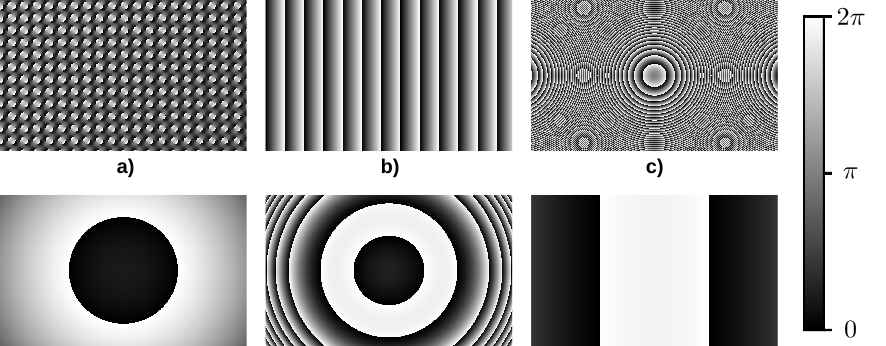
\includegraphics[width=\textwidth]{figures/hologram.png}
	\caption{
		Total phase mask applied on the SLM: \textsf{\textbf{a)}} Hologram obtained from the \ac{GSW} algorithm to generate the spot array.
		\textsf{\textbf{b)}} Lens phase applied to use the SLM as the first lens of a telescope with magnification $M=0.42$.
		\textsf{\textbf{c}} Optical flatness correction pattern as provided by the manufacturer.
		\textsf{\textbf{d)}} Blazed grating, used to move the diffraction pattern away from the optical axis (zoomed in).
		\textsf{\textbf{e)}} Aberration correction phase applied onto the SLM, which is a fourth-order polynomial in the distance from the center.
		\textsf{\textbf{f)}} Cylindrical lens phase to account for aberration introduced by the SLM itself.
	}
	\label{fig:SLMphase}
\end{figure}

In addition, apart from higher diffraction orders, there will always be a fraction of light that is not modulated.
This light originates from surface reflections, back reflections and unused space between the pixels and is focused to a single spot in the glass cell by the objective \cite{Bijnen2013}.
To get rid of this undesired light, typically a linear phase is superimposed on top of the hologram (tilt aberration) which translates the desired pattern away from the undiffracted light.
The type of linear phase used is shown in \cref{fig:SLMphase}d, as well as the hologram producing the spot array in \cref{fig:SLMphase}a.
Subsequently, in an intermediary focus point, the light can be spatially filtered to remove unwanted light using an iris. 
The Fresnel lens phase applied onto the SLM is shown in \cref{fig:SLMbeampath}b.
It is worth noting that this method comes at the cost of a slightly lower diffraction efficiency, because the phase ramp applied can only be approximated by the pixelated SLM.

\subsection{Beam size decrease}

To prevent excess loss of power, the $w = 4.8$ mm beam needs to be adapted to the $R = 2.0$ mm radius of the microscope objective. 
Thus the beam should be magnified by a factor $M=0.42$ (demagnified).
This is commonly done using a Keplerian telescope using two lenses $f_1$ and $f_2$ as shown in \ref{fig:SLMbeampath}a.
Moreover, apart from adapting the beam size, the telescope serves two more functions:

\begin{itemize}
    \item Conjugate the SLM plane and objective aperture planes.
    This means that for any arbitrary angular pattern applied by the SLM, the light field will remain centered on the circular objective aperture \cite{Nogrette2014}. 
    
    \item Allow for spatial filtering: the intensity profile is only produced in the focal plane of a lens (\cref{sec:InFocus}).
    Thus to remove unwanted light from unwanted diffraction orders, an intermediary focus plane is needed which is provided in any case when using a telescope.
\end{itemize}
To accommodate room for the objective holder, (dichroic) mirrors, a polarizing beam splitter cube leave room for additional optics in the future, we estimate from a CAD drawing we need $\sim 45$ cm of room between the last relay lens of the telescope and the objective. 
Using a Keplerian telescope, this distance will be equal to $f_2$ (\cref{fig:SLMbeampath}).

Also knowing that $f_1=f_2/M$ and the total length of the telescope is $2f_1+2f_2$, this is already $\sim 305$ cm of beam path on the optical table. 
Instead, we borrowed a trick from our collaborators at the University of Amsterdam, where we use the SLM as the first lens of the system. 
In terms of the ABCD matrix formalism, the transfer matrix $\mathbf{M}$ for the latter is:

\begin{figure}
	\centering
	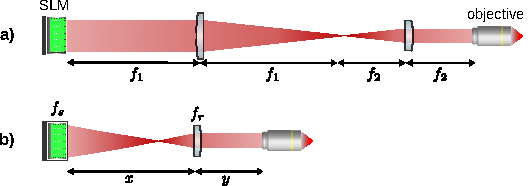
\includegraphics[width=0.9\textwidth]{figures/beampathSLM.pdf}
	\caption{\textsf{\textbf{a)}}: Keplerian telescope with total length $2f_1+2f_2$. \textsf{\textbf{b)}} Using the SLM as a lens, the total beam path has length $x+y$. In the latter case, $y>f_2$.}
	\label{fig:SLMbeampath}
\end{figure}

\begin{equation}\label{ABCD}
	\mathbf{M}=
	\begin{pmatrix}
		1 & y \\
		0 & 1
	\end{pmatrix}
	%
	\begin{pmatrix}
		1 & 0 \\
		-1/f_2 & 1
	\end{pmatrix}
	%
	\begin{pmatrix}
		1 & x \\
		0 & 1
	\end{pmatrix}
	%
	\begin{pmatrix}
		1 & 0 \\
		-1/f_1 & 1
	\end{pmatrix}.
\end{equation}
For substituting $x= f_2(1+f_1/f_2)$ and $y=f_2(1+f_2/f_1)$, \cref{ABCD} reduces to

\begin{equation}
	\mathbf{M}=
	\begin{pmatrix}
		-f_1/f_2 & 0\\
		0 & -f_2/f_1
	\end{pmatrix}.
\end{equation}
Which is the ABCD matrix for a beam expander. The total length is $x+y = 102 + 42.5 = 145$ cm for $f_2 = 300$ mm and $f_2/f_1=0.42$.
The Fresnel lens hologram used on the SLM (which is a quadratic polynomial) is shown in \ref{fig:SLMbeampath}b.
This pattern is superimposed on the spot array hologram in \ref{fig:SLMphase}a along with the other holograms described in this section. 
The sum of the hologram is computed modulo $2\pi$, which equals exactly one wave retardation.



\subsection{Optical Flatness}\label{subsec:Flatness}

Because of manufacturing imperfections, the SLM chip will not be perfectly flat on the scale of the wavelength of the light used. 
The exact shape of the chip area is slightly different between individual SLM units.
The flatness of our chip was measured by manufacturer Meadowlark to have a RMS flatness of $\sim 0.18\lambdaup$ (785 nm).
The shape of the flatness was measured as well and provided to us by the manufacturer, so we can correct for it by subtracting a phase mask corresponding to the same non-flatness.
This mask is shown in \ref{fig:SLMphase}c.


\subsection{Aberration Correction}\label{subsec:AberrationCorrection}

Now that the SLM has been introduced, we will explain more thoroughly how exactly we corrected for spherical aberration as introduced by the incorrect glass thickness (\cref{sec:Tweezer3D}).
We left off at \cref{eq:SphericalFocus}.
For paraxial rays ($\alpha_0 \rightarrow 0$), \cref{eq:SphericalFocus} reduces to $d(1-n_r)$. 
Subtracting this paraxial result from the case for general ray angles, which may contain large angles from \cref{eq:SphericalFocus} and Taylor expanding up to fourth order in $\alpha_0$ yields the difference in focus shift between the general and paraxial case of \cite{Iwaniuk2011}

\begin{equation}\label{eq:FocusDifference}
    \delta f_{\text{general}} - \delta f_{\text{paraxial}} \approx
    -\frac{d \tan^2{\alpha_0}}{2n} (1-n_r^2) 
    +\frac{3d \tan^4{\alpha_0}}{8n}(1-n_r^2)^2+\mathcal{O}(\tan\alpha_0^6).
\end{equation}
Multiplying \cref{eq:FocusDifference} with $2\pi(n-n_0)/\lambdaup$ and converting to a radial dependence as $\tan{\alpha_0}= \text{NA} \times r/R$ yields 

\begin{equation}\label{eq:ConversionRadial}
    \phi(r) \approx \frac{\pi d}{\lambdaup}(1-n_r)\left[
    -\left(\text{NA}\frac{r}{R}\right)^2(1-n_r^2)+\frac{3}{4}\left(\text{NA}\frac{r}{ R}\right)^4(1-n_r^2)^2
    \right].
\end{equation}
This is a function that can be decomposed in Zernike polynomials.
The Zernike polynomials are a set of orthogonal polynomials on the unit disk, related to optical aberrations. 
The coordinates on the unit disk can be denoted as $\rho = r/R$ and $\theta \in (0, 2\pi)$, such that the wavefront $\phi(\rho,\theta)$ can be expanded in terms $R_n^m(\rho)\cos{m\theta}$ and $R_n^m\sin{m\theta}$ where 

\begin{equation}\label{eq:ZernikeRadial}
    R_{n}^{m}(\rho)=
    \sum_{s=0}^{(n-m) / 2}
    \frac{(-1)^{s}(n-s) !}{s !\left((n+m)/2-s\right) !\left((n-m)/2-s\right) !} \rho^{n-2 s}
\end{equation}
is the radial Zernike polynomial set \cite{Mahajan94}. 
Expanding \cref{eq:ZernikeRadial} in radial Zernike terms yields

\begin{equation}\label{eq:ZernikeExpansion}
    \phi(\rho) \approx 0.254 \cdot Z_0^0 - 12.9 \cdot Z_2^2 + 0.254\cdot Z_4^0.
\end{equation}
\begin{figure}
    \centering
    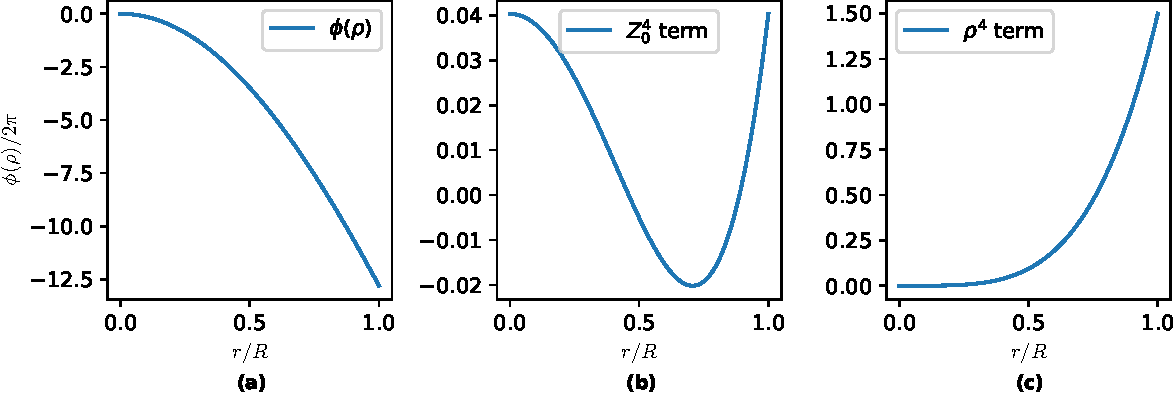
\includegraphics[width=\textwidth]{figures/SphericalAberrationTerms.pdf}
    \caption{
    Radial Zernike polynomials in terms of the normalized radial coordinate $\rho = r/R$.
    \textsf{\textbf{a)}} Total phase error from \cref{eq:ZernikeRadial}.
    \textsf{\textbf{b)}} Only the spherical aberration component of \cref{eq:ZernikeRadial} $z_0^4$, which is actually applied onto the SLM.
    \textsf{\textbf{c)}} Only the $\rho^4$ component, which in terms of Zernike is actually a $Z_4^4$ polynomial.
    }
    \label{fig:AberrationTerm}
\end{figure}
Which is plotted in \cref{fig:AberrationTerm}a.
But we do not need to correct for the full wave error: the $Z_0^0$ is a constant offset phase term. 
Adding a constant has no effect so we can omit it. 
The $Z_2^2 = \rho^2$ term is a defocus aberration, which we can also omit: it is unnecessary to correct for the shift in focus of the glass, we can do this by moving the objective. 
That leaves the $Z_4^0 = 1 - 6\rho^2+6\rho^4$ term (primary spherical aberration) plotted in \cref{fig:AberrationTerm}b \footnote{Because the pupil of the microscope objective is conjugated with the short axis of the SLM, the radial coordinate $\rho =r/R$ also happens to apply on the SLM surface, if one substitutes $R=S_y$ (the short axis of the rectangular aperture).}.
This primary spherical aberration was applied onto the SLM, its corresponding hologram is shown in \cref{fig:SLMphase}e.
Note: the primary spherical aberration term can again be expanded if one wishes to do so: only its $\rho^4$ term is relevant for us, which is plotted in \cref{fig:AberrationTerm}c. 


Even after the spherical aberration correction, we still noted unsatisfactory performance in the axial direction as discussed in \cref{sec:Tweezer3D}. 
We think this is due to the lens phase on the SLM (\cref{fig:SLMLens}b): because the laser reflects off of the device, it effectively travels through a biconvex lens under this same angle (astigmatism aberration). 
This can cause the focus position to change slightly between $x$ and $y$, which would explain the increased Rayleigh range measured. 
We corrected for this by applying an additional lens phase only in the horizontal direction as shown in \cref{fig:SLMphase}f.


\section{Characterizing Tweezer Arrays}\label{sec:ArraysResults}

Using the \ac{GSW} algorithm implemented in Python code by Ivo Knottnerus, we generated holograms corresponding to $n \times n \times 1$ pixels in the $x$, $y$ and $z$-directions respectively, where $n = 1,2,\ldots 10$ (larger arrays are possibly, but cannot be fully imaged onto the CCD camera used because of the limited field of view in conjunction with the 0.85 NA objective). 
The algorithm was run until the uniformity $u$ reached 0.999. 
A typical hologram that was obtained is shown in \cref{fig:SLMphase}a.
Here, an example for a $7 \times 7$ array was used. 
In \cref{fig:SLMphase}b, the simulated diffraction pattern from this phase mask is shown. 
The units in this Fourier plane are so-called focal units, which are the Fourier transformed coordinates \cite{Bijnen2015}



\begin{figure}
    \centering
    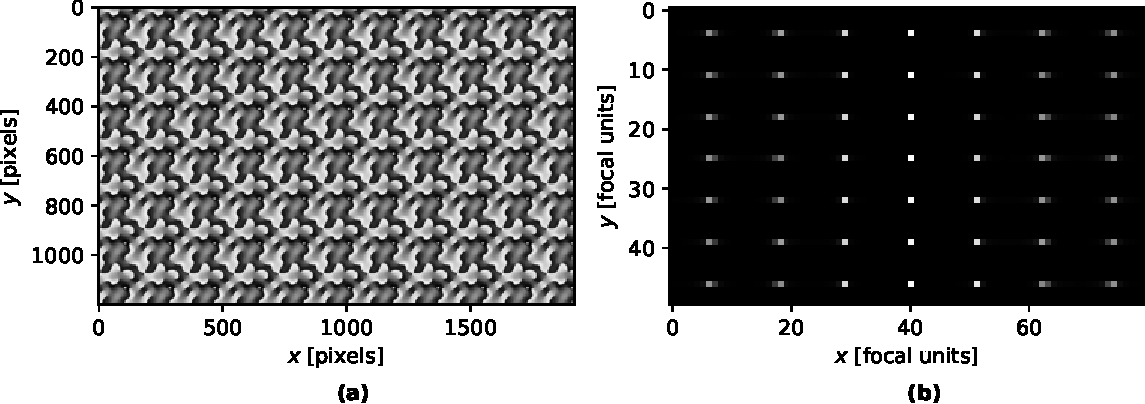
\includegraphics[width=\textwidth]{figures/MaskAndComputedPattern.pdf}
    \caption{\textsf{\textbf{a)}} Hologram computed by the \ac{GSW} algorithm to compute a $7\times7$ spot array.
    \textsf{\textbf{b)}} Diffraction pattern as computed from the algorithm using the hologram in \textsf{\textbf{(a)}} in focal units (\cref{eq:FocalUnit}.}
    \label{fig:HologramPattern}
\end{figure}

\begin{equation}\label{eq:FocalUnit}
    \Delta x \times \Delta y = \frac{\lambdaup f}{S_x}\times \frac{\lambdaup f}{S_y},
\end{equation}
where $S_x = 7.7$ mm and $S_y = 4.8$ mm are the semi-widths of the rectangular SLM aperture in $x$ and $y$ directions respectively.
Multiplying the spacing in focal units in \cref{fig:HologramPattern} with the definitions in \cref{eq:FocalUnit} will lead to a uniform spacing of $\sim 5$ $\mu$m in the Fourier plane. 
Because of non-integer spacing in focal units of the target pattern and the pixelated nature of the array of focal units in \ref{fig:HologramPattern}b, for some spots the peaks are spread out over multiple pixels, but this has no effect on the hologram itself: in the diffraction equation \cref{eq:Vm} the diffraction-limited spot area is considered, which does not have to line up with the pixels in \cref{fig:HologramPattern}b.

The $7\times7$ array as measured on the camera is shown in \cref{fig:CameraLoG}, where the only relevant section of the CCD chip is shown. 
We are mainly interested in the uniformity of the array, as well as the spot size.
To do this, we performed 2D Gaussian least-square fits (\cref{eq:2DGaussian}) as a function of the spot labeled $m$.

\begin{figure}
    \centering
    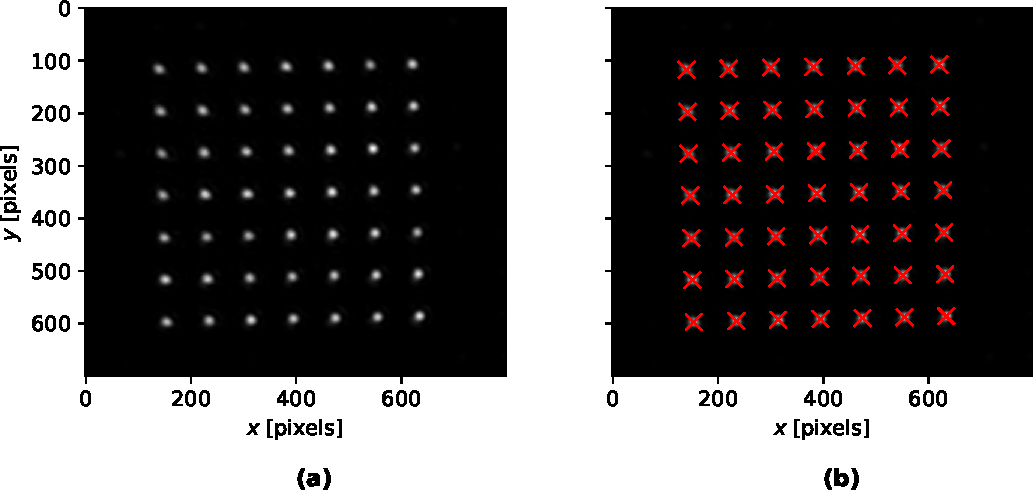
\includegraphics[width=0.95\textwidth]{figures/CamImgLoGSpots.pdf}
    \caption{\textsf{\textbf{a)}} $7\times7$ spot array as obtained from the Flea2 CCD chip.
    \textsf{\textbf{b)}} Spot locations marked with the red crosses, as obtained from the edge-detection algorithm. }
    \label{fig:CameraLoG}
\end{figure}

\begin{equation}\label{eq:2DGaussianNumberK}
    U_m(x,y) = U_{0,m}\exp{\left(\frac{-(x_m-x_{0,m})^2}{2\sigma_{x,m}^2}\right)}
    \exp{\left( \frac{-(y_m-y_{0,m})^2}{2\sigma_{y,}^2} \right)}.
\end{equation}
The fit is similar to the one shown in \cref{fig:3Dshowing}.
Each fit of spot $m$ has 5 fit parameters: the amplitude (optical trap depth) of the Gaussian: $U_{0,m}$, the center of the potential $(x_{0,m}, y_{0,m})$ and lastly the spread of the Gaussian in Cartesian coordinates $\{\sigma_{x,m},\sigma_{y,m}\}$.
Similar to the single tweezer of the previous chapter, the waist is obtained as $w_{0,m} = \sigma_{x,m}+\sigma_{y,m}$, a assumption valid for $\sigma_x\sim\sigma_y$.

In order to routinely perform each fit, a starting guess for the center of each potential is needed, after which a \ac{RoI} can be extracted similar to \cref{fig:3Dwaistfit}.
To reliably detect the expected number of spots, we used the \ac{LoG} edge detection algorithm \cite{Haralick1992}. This method works by computing the Laplacian of the discrete pixel array, where zero crossings above a certain threshold in the second derivative are marked as an edge (spot). 
To prevent marking noisy pixels as a peak, the array is convolved with a Gaussian filter first. 
The spots found by the algorithm are marked in \ref{fig:CameraLoG}b by red crosses. 
If the detected number of spots is too little or too high, the detection threshold can be adjusted, which we did not find to be necessary in practice. 

In \cref{fig:SpotsRoI}, the extracted \ac{RoI} by the \ac{LoG} algorithm is shown for the first 3 peaks. 
Subsequently, the center of the peaks as found by the 2D fit $(x_{0,m},y_{0,m})$ is marked with the red dot, where the $1/e^2$ radii are marked by circles. 
Subsequently, the extracted fit parameters can be used to perform some statistics.
Histograms of the obtained waist (left) as well as trap depths (right) for the same $7\times7$ array are presented in \cref{fig:Histograms}.
We fitted the data in the histograms to a normal distribution, yielding a waist of $w_0 = (0.89 \pm 0.03)$ $\mu$m, where the error denotes the standard deviation, and not the uncertainty in the calibration of the magnification. 

\begin{figure}
    \centering
    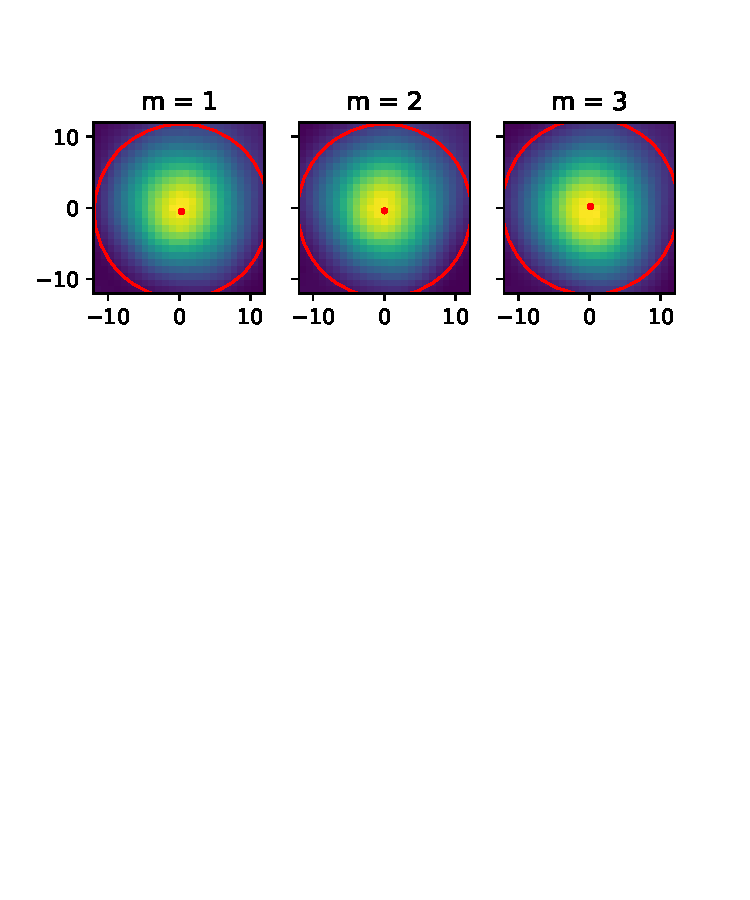
\includegraphics[width=0.6\textwidth]{figures/SpotsCropped_range12.pdf}
    \caption{Region of interest in pixels around the first 3 spots, as extracted by the Laplacian of Gaussian. 
    The centers $(x_{m,0},y_{m,0})$ as found by the 2D is shown by the red dot. 
    The obtained $1/e^2$ radius $w_{m,0}$ is denoted by the circles is drawn for each peak $m$ as well.}
    \label{fig:SpotsRoI}
\end{figure}



\begin{figure}
    \centering
    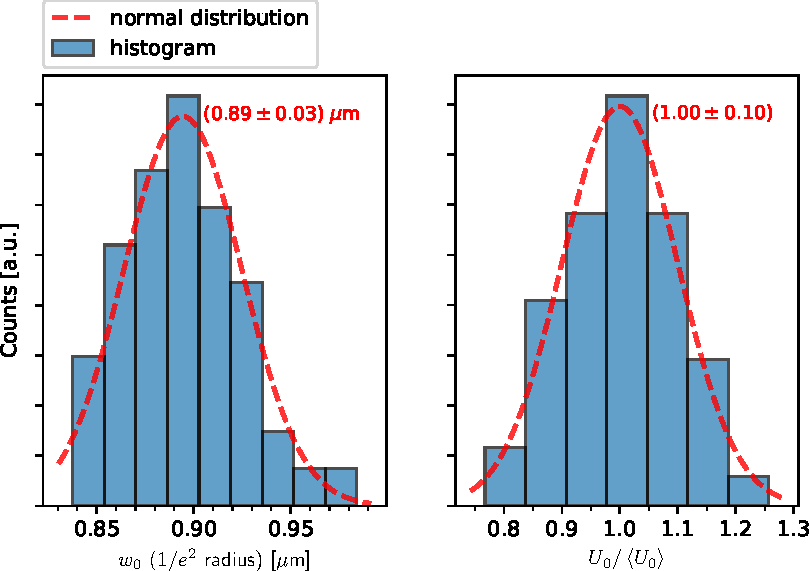
\includegraphics[width=0.85\textwidth]{figures/FittedHistograms.pdf}
    \caption{\textsf{\textbf{a)}} Distribution of the $1/e^2$ radius as measured from the spot array in \cref{fig:CameraLoG}a.
   \textsf{\textbf{b)}} Spread in the fitted depth of the potential $U_0$, normalized by the average trap depth $\left\langle U_0 \right\rangle$.
    Both are fit to a normal distribution.
    }
    \label{fig:Histograms}
\end{figure}

\subsubsection*{Homogeneity}

As a result of the slightly varying waist, there will also be a non-homogeneity (uniformity) in the intensities (trap depths) of the array.
There are other causes to the spread in uniformity as well.
For example, the diffraction efficiency of the SLM increases as one gets closer to the optical axis approximately as $\operatorname{sinc}^2\{
\pi/2 (\theta_{\text{m}}/\theta_{\text{m,max}})\}$ where $\theta$ is the deflection angle from the zeroth order \cite{Ebadi2021}.
We neglected this effect for now: because quite a strong separation phase ramp was used, this variation will be small.

The spread in trap depths is shown in \cref{fig:Histograms}.
Because we only care about the spread and not about the magnitude of the intensity (the former is dependent on camera sensitivity, dichroic filters and laser power used), we normalize by the average trap depth $\left\langle U_0 \right\rangle$, yielding for this array a spread of $\sim 10$\%, which we found to be fairly typical irrespective of the amount of spots in the array.
To our knowledge, there is no literature result of the measurement method used here to compare to, because in a cold atom experiment it is usually measured by an imaging system of similar \ac{NA} by

\begin{enumerate}
    \item Placing the camera after the glass cell. 
    In our case that the camera would have to be accompanied be an identical long-working distance microscope, to bridge the 30 mm outer thickness of the cell.
    This is the same principle as using a set of two in-vacuum high-NA aspheric lenses as done by \cite{Nogrette2014}.
    
    \item Separating Stark-shifted atomic fluorescence from ultra-cold atoms in tweezers recorded by the same high-NA lens used to produce the tweezer array \cite{Ebadi2021}.
\end{enumerate}
In both cases, the light travels twice through the high-NA lens and vacuum glass, which typically seems to yield a larger spread: \cite{Nogrette2014} found 19\% standard deviation uniformity whereas we found $10\%$.

As also shown by \cite{Nogrette2014}, it is also possible to improve this uniformity by iteratively adapting the weight factors in the \ac{GSW} algorithm in a feedback loop to achieve a non-homogeneity of $1.4\%$.
It is worth noting here that this correction can only be as good as the imaging system used to obtain the feedback. 
Thus, in the method 1) one has to be careful not to 'over-correct' for aberrations \cite{Labuhn2016}, as it is impossible to know if the aberrations really occur in the place of the atoms or are rather a result of the imaging system which will also have aberrations. 
Because of this, the latter method 2) of really looking at the Stark shift by the atomic fluorescence might be the more robust method because here the aberration picked up by the imaging system will be approximately the same aberration introduced by producing the tweezer array in the first place (as the same high-NA lens is used.)
Both methods 1) and 2) are possible to implement in our ultra-cold experiment, which we will introduce now.








    
\chapter{Implementation in the Machine}\label{ch:implementation}
    %Now that the light potentials have been measured, we elaborate in this chapter how it was implemented in an real-world experiment on ultra-cold atoms, initially using Rb atoms.
While our group has a lot of experience on Rb magneto-optical traps, because of the use of a glass cell and microscope objectives, we built a novel apparatus almost from scratch, apart from the laser system which we used from the previous setup.
The construction of the vacuum and atom source part can be found in \cref{sec:VacuumAtom}.
The laser system is explained in \cref{sec:LaserSystem}.
Images of the MOT are displayed in \cref{sec:MOTresult}.
We finish up with how overlap this MOT with our tweezer array (\cref{sec:Tweezers}) and how to image the tweezers (\cref{sec:TweezerImaging}).

\section{Vacuum and Atom Source}\label{sec:VacuumAtom}

The vacuum and atom source of the setup was designed with compactness in mind. 
The core of the experiment is the glass cell (30 mm outer and 4.0 mm wall thickness, optically contacted)\footnote{The glass cell was provided to us by our collaborators from the University of Amsterdam.}.

The microscope objectives are place in the vertical direction.
The coils producing the magnetic field gradient should also be placed near the cell. 
To still have room for all 6 MOT beams, we use a design similar to the \textit{Endres} group.
The idea is that two MOT beams and their retro-reflection pass the cell under a 60 degree angle, leaving room for the microscope objectives. 
The last MOT beam is sent through the hole of the anti-Helmholtz magnetic field coils.
To allow for placement of optics in the vertical direction, a vertical was used. 
In \cref{fig:VacuumSetup} the vertical breadboard is shown along with the vertical MOT beams and the magnetic field coils. 
Also the bottom objective is shown. 
The center of the glass cell is positioned 110 mm away from the vertical breadboard and 300 mm from the optical table. 
The housing for the magnetic field coils was designed by Deon Janse van Renseburg and Rick van Herk and is shown in \cref{fig:Coils} in \cref{subsec:Overlap}.

A real life picture of the glass cell is shown in \cref{fig:Chamber}.
It is pumped down to the ultra-high vacuum regime, which is need to minimize collisions with the background gas and improve the lifetime of the atoms in the tweezers.
To pump the cell down, the glass cell is connected to a vacuum chamber (\cref{fig:VacuumSetup}, left).
To allow for more room around the glass cell, in between the vacuum vessel and the glass cell an extension tube is added.
We attach a turbomolecular pump to the chamber using a valve (not shown in the figure) and pump down to $\sim 10^{8}$ mbar.
This pressure was measured using a pressure Gauge (\cref{fig:Chamber}).
To reach a better vacuum, the system was baked for a duration of two weeks at 130${}^{\circ}$C by Rik van Herk \cite{Herk2022}.

As atom source, a Rb dispensers\footnote{SAES Getters Alkali Metal Dispensers.} is used.
Only one dispenser is connected at a time, but we installed a triplet for redundancy.
The amount of Rb released can be controlled by the current running through the dispensers.
We typically run the dispensers at $\sim$ 5A.
The dispensers are mounted to the vacuum chamber using a CF40 adapter made by Eddy Rietman.
We first ran the dispensers for 30 minutes while leaving the turbo pump on to get rid of the oxidation layer on the dispenser.
This lead to a brief but significant increase in pressure, while we say no atomic fluorescence from Rb in the chamber.  
Next, we activate the non-evaporative getter\footnote{NEXTorr Z 100 NEG - ion combination pump.} by heating it to 500${}^{\circ}$C while pumping away its out gassing using the turbo pump. 
Finally, after closing the turbo valve and turning on the ion pump we reached a pressure of $\sim 2\times 10^{-10}$ mbar, as measured using the ion pump (the pressure gauge is not usable in this pressure regime).
When turning on the dispensers, the pressure briefly spikes to the $10^{-9}$ region but quickly returns back to the $10^{-10}$ regime.
One note: if this Rb machine is to be used for a longer time in the future, it would probably be wise to add a valve between the dispensers and the vacuum vessel, which allows for replacement of the dispensers without venting the entire chamber. 


\begin{figure}
	\begin{subfigure}{.5\linewidth}
		\flushleft
		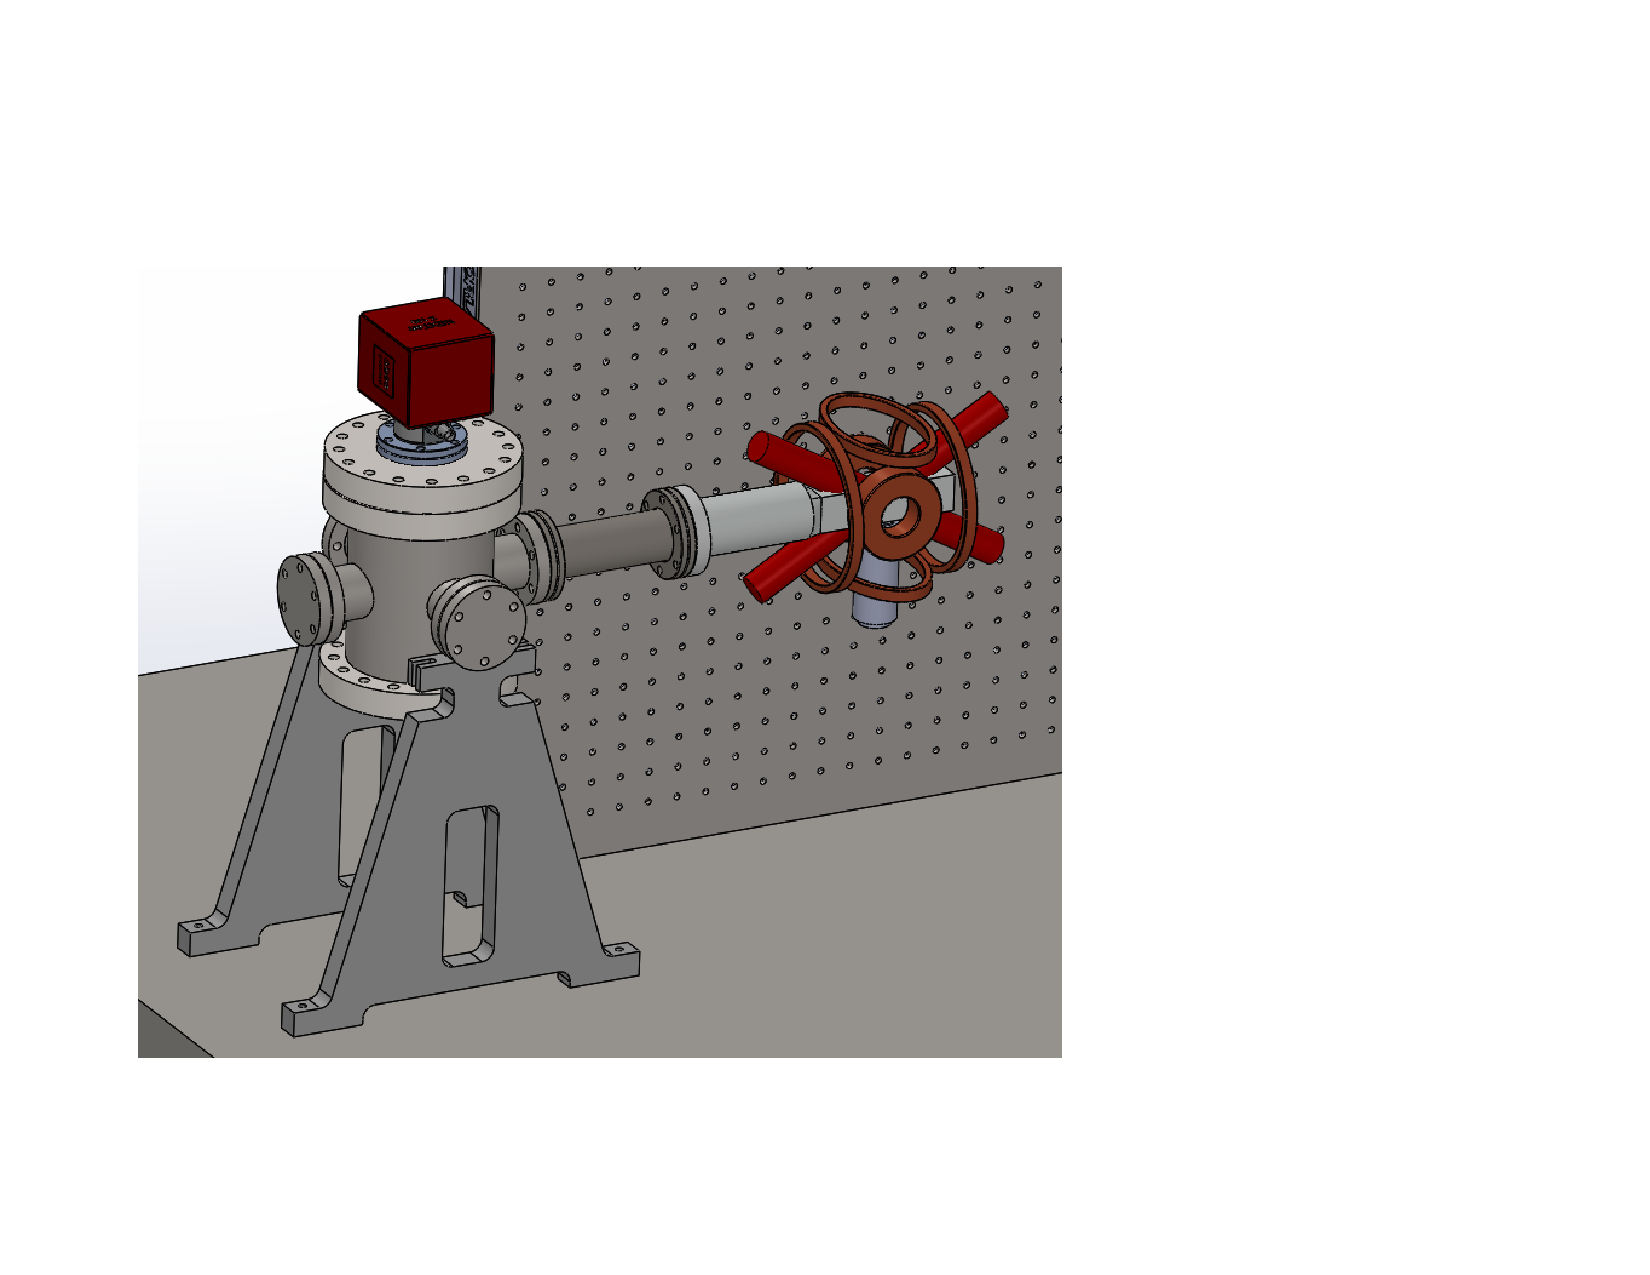
\includegraphics[height=6.5cm]{figures/Vacuum.pdf}
		\caption{}
		\label{fig:VacuumSetup}
	\end{subfigure}
	\hfill
	\begin{subfigure}{.49\linewidth}
		\flushright
		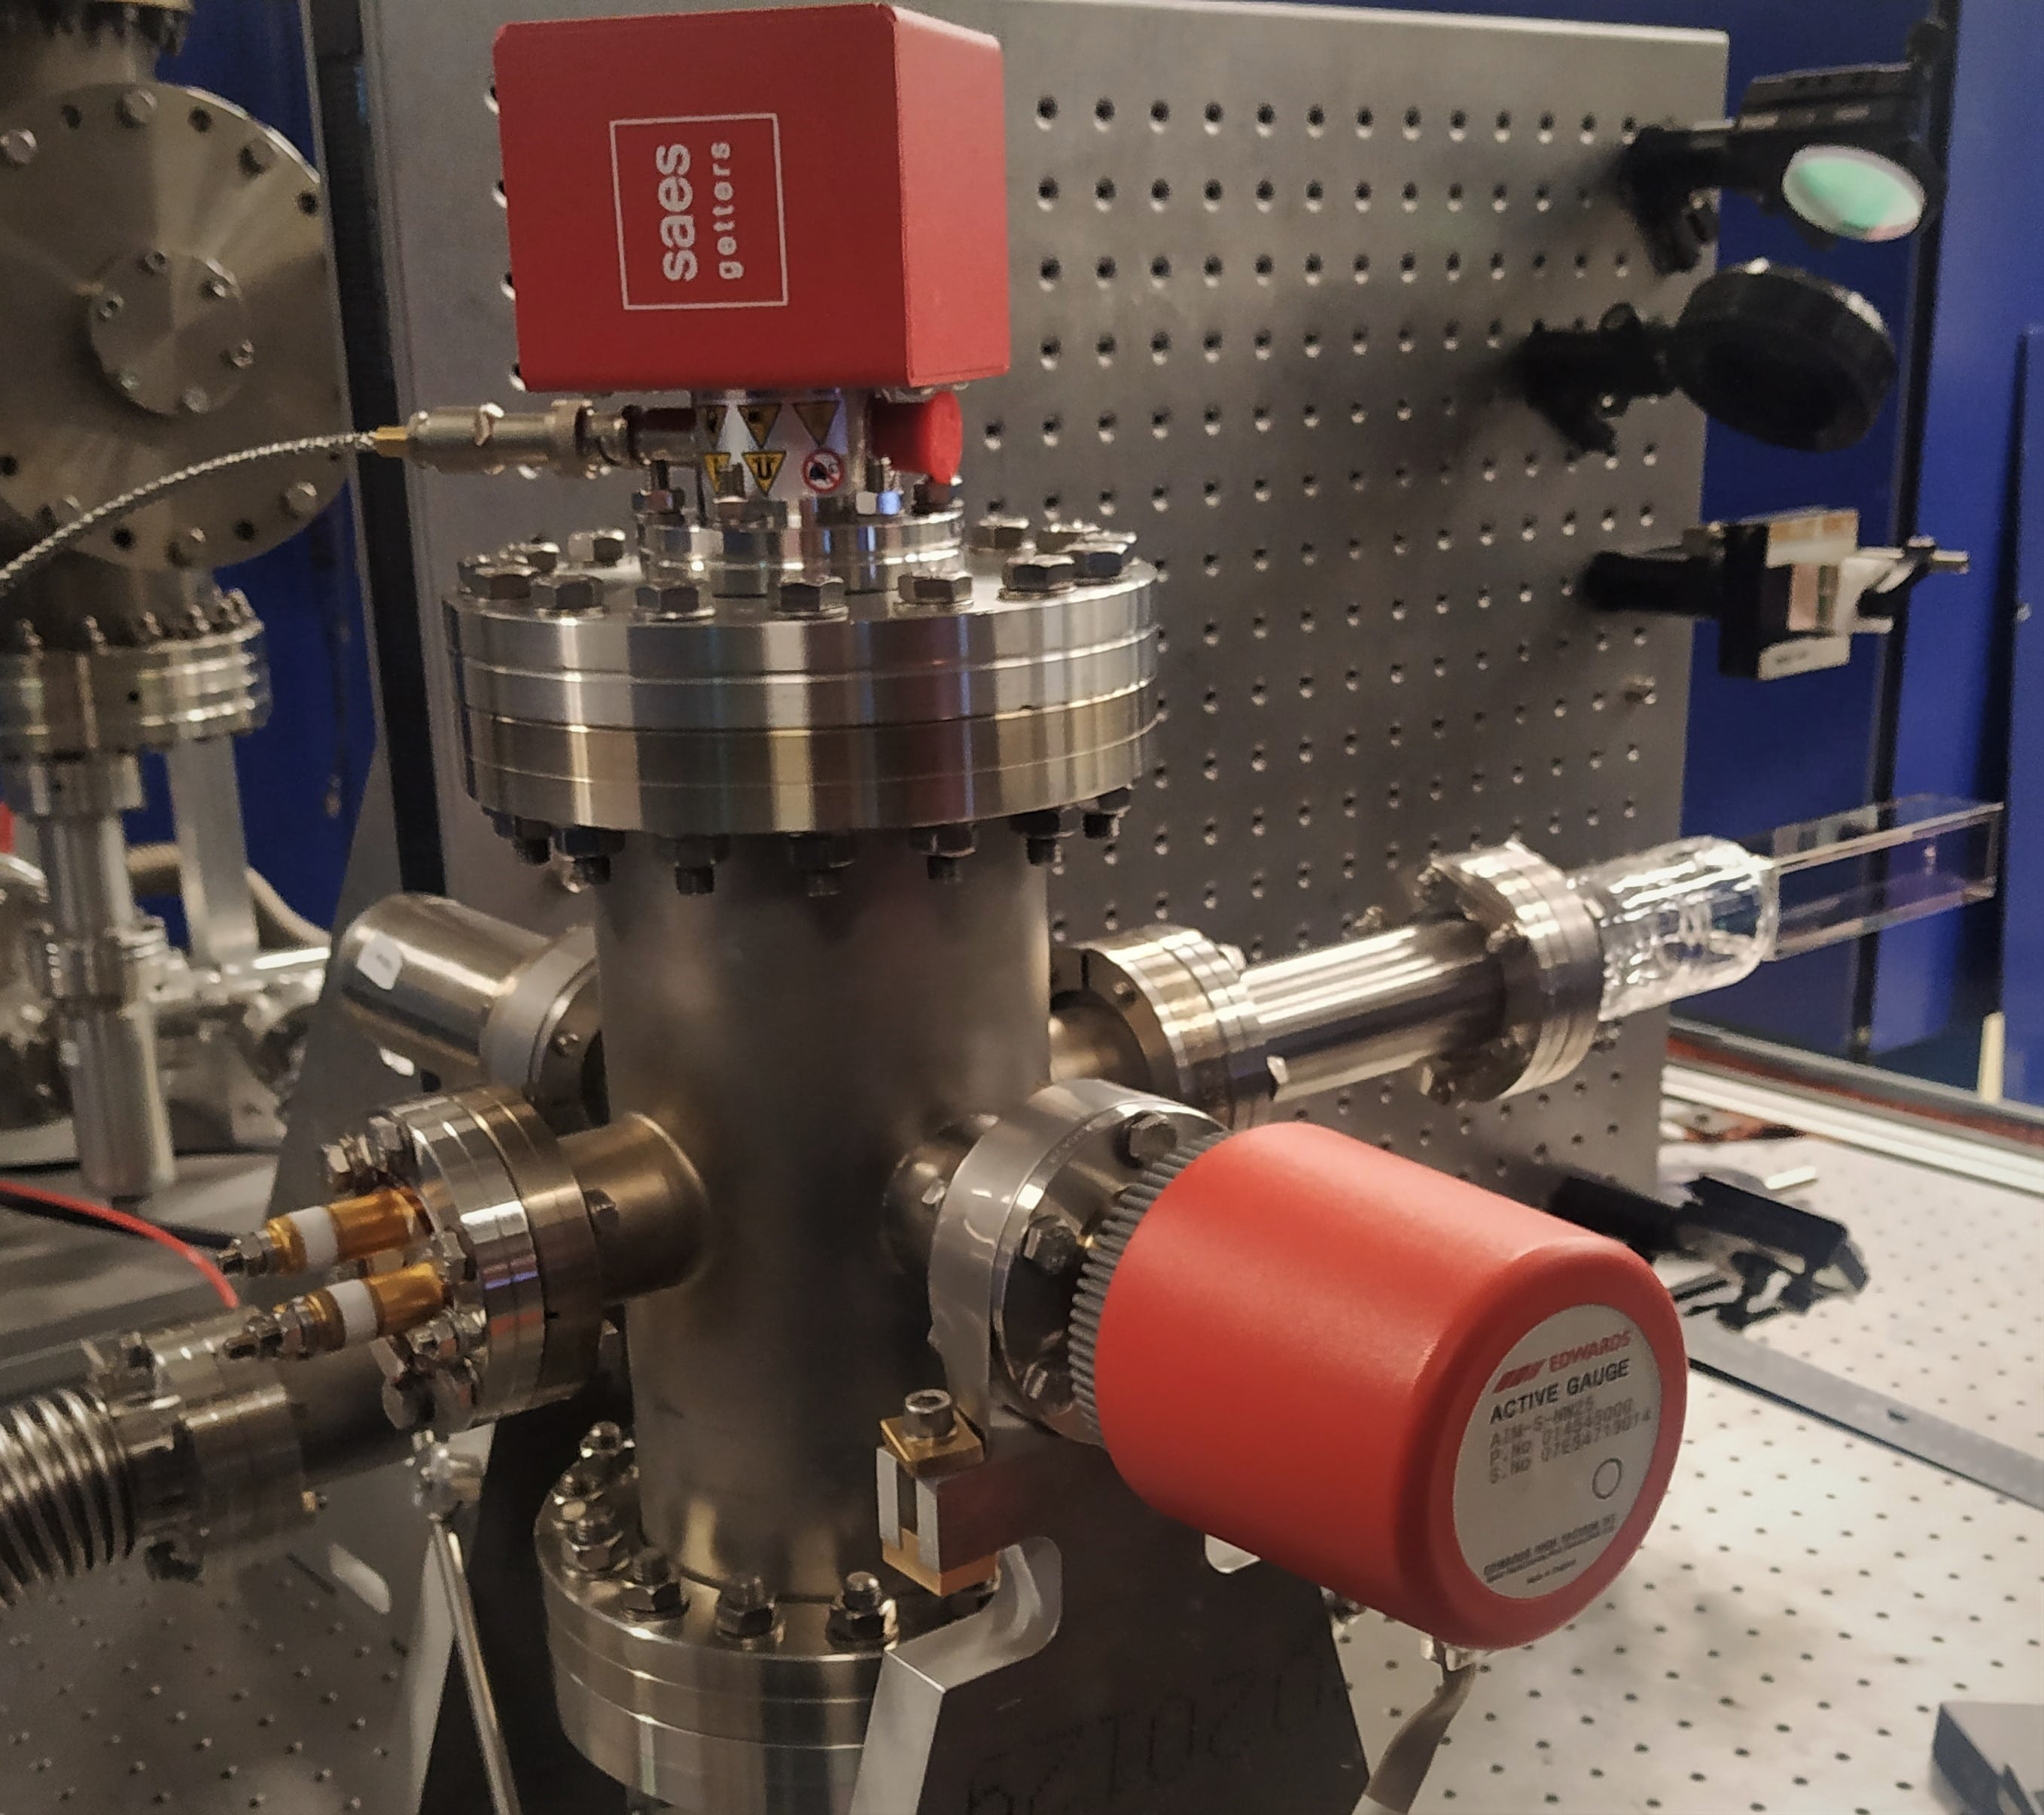
\includegraphics[height=6.5cm]{figures/Chamber.jpg}
		\caption{}
		\label{fig:Chamber}
	\end{subfigure}
	\caption{\textsf{\textbf{a)}} CAD drawing of the vacuum vessel connected to the glass cell on the right. 
	Around the glass cell, 4 out of 6 MOT beams are shown along with the magnetic field coils and a single microscope objective on the bottom. 
	CAD drawing by Eddy Rietman.
    \textsf{\textbf{b)}} Picture of the vacuum components: top: ion/getter pump. Right: glass cell. Also connected to the chamber rom left to right: valve for turbo pump, triplet of Rb dispensers and pressure gauge.}
\end{figure}

\section{Laser System}\label{sec:LaserSystem}

For the laser system we recycled a significant part of the previous setup \cite{Reijnders2010}.
The atomic species we selected is Rb-85 because it is the most abundant isotope. 
a Rb-85 MOT requires two lasers: a trapping/cooling laser as well as a repump laser to recycle back atoms that end up in the wrong ground state (\cref{sec:PracticeRb}).
We used the same laser source for both of them. 

\subsection{Cooling/Trapping}

For the laser cooling and trapping beams we used the Toptica DLX110.
This laser should be able to produce $\sim 1$ W of power, but in current condition we typically output $\sim 500$ mW, which is already plenty of power for what we need. 
The repump light is produced by applying sidebands of fixed frequency spacing on the main trapping laser, more on this later.

\begin{figure}[t]
    \centering
    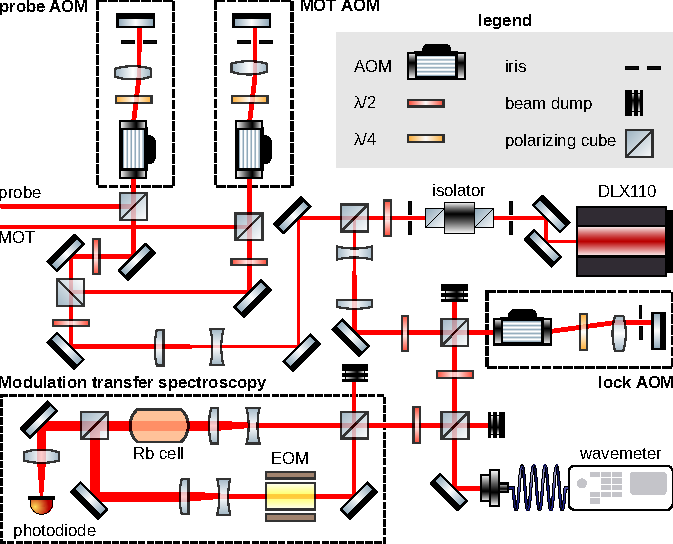
\includegraphics[width=\linewidth]{figures/RbLaserSetup.pdf}
    \caption{Laser system for the trapping and repump laser system for \textsuperscript{85}Rb.
    This system was built by \cite{Reijnders2010}.
    A section of laser light is split off to the modulation transfer spectroscopy (bottom left), after first double passing the lock \ac{AOM} (right). 
    Top: set of AOMs for the MOT and probe light.
    }
    \label{fig:RbLaserSetup}
\end{figure}

The laser is shown in \cref{fig:RbLaserSetup}.
After passing an optical isolator, a fraction of laser power is split off to the modulation transfer spectroscopy section after being offset-locked using the lock \ac{AOM} (right) set to $2\pi \times  84.5$ MHz\footnote{From now on, all frequencies are assumed to be angular and we omit the $2\pi$ term.}
Modulation transfer spectroscopy is described elsewhere \cite{McCarron2008,Reijnders2010}, but very briefly: the working principle is that by scanning the probe pulse using the \ac{EOM}, the absorption peak of $D_2$ is found using the Rb cell, which the laser is locked to.  
Contrary, the MOT AOM (top) is set to 80 MHz, which is $2 \times (80 - 84.5) = -9$ MHz from the resonance frequency, which is roughly equivalent to a detuning of $\delta = -1.5 \gamma$.
We typically use about $80$ mW of power for the MOT beams as measured after the \ac{AOM} in \cref{fig:RbLaserSetup}.
We have another AOM, which we use to make probe light, the light to induce fluorescence of the atoms when they are trapped in the optical tweezers.
The probe light is better described in \cref{sec:TweezerImaging}.

\begin{figure}[t]
    \centering
    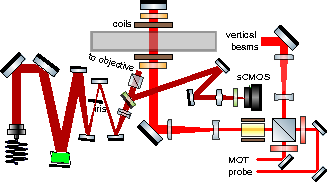
\includegraphics[width=\textwidth]{figures/MOTupview.pdf}
    \caption{The laser for the MOT beams and probe beam are split to a vertical beam section (see \cref{fig:GlassCellSide}) as well as one horizontal beam, which travels through the anti-Helmholtz coil as shown here. 
    Both beams are expanded using a beam expander.
    This horizontal beam also contains the repump light using the \ac{EOM}.
    }
    \label{fig:GlassCellTop}
\end{figure}

\subsection{Repump}

Contrary to the previous setup, we do not use a separate repump laser. 
Instead, we used an \ac{EOM}.
The principle at play here is the electro-optic effect that can be used to modulate a beam of light. 
We drive the EOM with a modulation amplitude $\epsilon$ and frequency $\Omega$.
If the laser beam is described by amplitude $A$ and frequency 'carrier' frequency $\omega = \omega$ as $A = A_0 e^{i \omega_c t}$, after passing through an EOM the amplitude can be described as

\begin{equation}
    A(t) = A_0 e^{i \omega t}(1+i \epsilon \sin(\Omega t)
\end{equation}
where we assumed $\epsilon < 0$. In this case ($\epsilon <0$), most of the power is still contained in the carrier frequency component $\omega_c$, but a small fraction of power is contained in two first-order sidebands at $\omega_c \pm \Omega$.
We can use one of the sidebands as our repump laser. 
The other side-band is unused. 

As for the experimental details.
The EOM\footnote{7Qubig EO-Rb85-3K} was fed a $\Omega = 2915$ MHz signal provided by a harmonic synthesizer RF\footnote{DS instruments SG6000PRO} providing a signal of $-6.9$dbm.
This signal was amplified by a 45 dB amplifier\footnote{Minicircuits ZHL-16W-43+} which should provide some $\sim 10$\% of power in the first sidebands \cite{Rens2014}, which should be a sufficient amount of power for a repump laser. 
We did not measure the exact fraction of power in the sidebands because we do not have a sufficiently high-finesse wavemeter available, but the current parameters seemed to work satisfactory. 

\subsection{Distribution the Beams}

After passing through the AOMs, the MOT and probe light beams are directed further to the glass cell. 
This is shown in \cref{fig:GlassCellTop}.
Both beams are combined in a polarizing beam splitter cube, which also serves to split the MOT beams: one branch going to the horizontal section as shown in \cref{fig:GlassCellTop} as well as a beam that serves as the angled vertical MOT beams, as shown in \cref{fig:GlassCellSide}. 
Both beam paths are expanded to increase the overlap volume of the resulting MOT beams.
This was done using Galilean beam expanders. 
The lenses used for the horizontal beam are $f=-75$ mm and $f=400$ mm, which for a $\sim 0.9$ mm initial beam comes down to $\sim 0.9 \times 400/75 \sim 4.8$ mm.
The beam expander for the horizontal beam expands the $\sim0.9$ mm beam waist a factor of $400/75$ to $\sim5.4$ mm.
The angles beams are slightly bigger: because they are angled they need to be to still have a sufficiently big overlap volume. 

The half wave plates in front of the cube are set to only have probe light in the horizontal beam, while about 2/3 of the power for the MOT beams will travel to the vertical section. 
The repump light is only present in the horizontal beam: as a result of hitting the glass cell perpendicularly this beam has only a few per cent reflection losses, contrary to the vertical MOT beams. 
Because we only need repump light in one of the beams, it thus makes sense to do in this horizontal beam. 
The horizontal beam travels through the anti-Helmholtz coils as shown in \cref{fig:GlassCellTop}.
The mirror and $\lambdaup/4$ plate for retro-reflection are mounted directly on the vertical breadboard. 

Furthermore, the probe light is only directed to the horizontal beam path as well. 
This because the probe is on during the imaging sequences and the horizontal beam has considerably less reflections, meaning less background. 
Typically we run about an intensity of $I \sim I_{sat} =1.6$ mW/cm${}^2$ in the probe beam.
The detuning is a couple linewidths from the Stark shifted tweezers. 

\begin{figure}
    \centering
    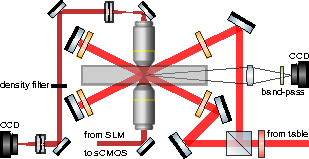
\includegraphics[width=0.85\textwidth]{figures/MOTsideview.pdf}
    \caption{Side view on the glass cell, showing vertical MOT beams under a 60 degree angle, as well as the bottom microscope objective. 
    The top and side view MOT cameras are shown as well.}
    \label{fig:GlassCellSide}
\end{figure}


\section{Characterizing the MOT}\label{sec:MOTresult}

To image the MOT we position a CCD cameras\footnote{UEye UI-2230SE} looking at the MOT from the side, using the 5th and last available glass cell window. 
The camera is positioned in an $X-Y-Z$ translation stage and features a 780 nm band-pass filter. 
This camera has a magnification of $0.5$ and has a $f=100$ mm lens. 
Having camera images from two perpendicular axes allows for spatial overlapping in three dimensional space, more about this in \cref{subsec:Overlap}.
The top windows of the glass cell is used by the identical Mitutoyo microscope objective. 
The objective is brought in focus with the tweezers and the MOT is overlapped with both microscope objectives, ensuring we are in focus.


A picture showing the laser-induced fluorescence from the MOT as imaged through the camera on the side is shown in \cref{fig:LiF}.
A Gaussian fit of the spatial profile in $x$ and $y$-directions is shown in \cref{fig:LiF}.
When moving the MOT with the compensation coils, we see the MOT seem to change shape. 
Probably, this is due to the compensation coils not being perfectly Helmholtz (their spacing is unequal to their radius). 
As a result, the Helmholtz pair that makes a field in the $y$-direction could also have $x$ and $z$ components, for example. We think that for us this is not really a problem, however.
For the image in \cref{fig:LiF}, we find a 

\begin{figure}
    \centering
    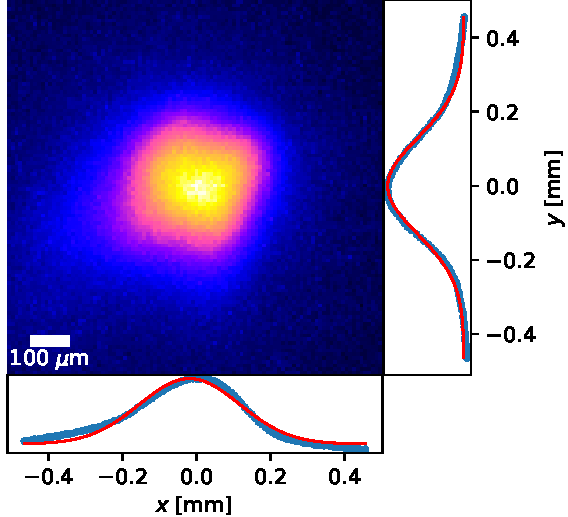
\includegraphics[width=0.65\textwidth]{figures/FluoresenceAndFits.pdf}
    \caption{A picture of laser-induced fluorescence from the magneto-optical trap as imaged onto side camera. 
    The colors denote the relative intensity.
    Also, a Gaussian fit is shown in the $x$ and $y$-directions.}
    \label{fig:LiF}
\end{figure}

   
We estimate the number of captured atoms in the MOT by counting the number of counts on our side camera, subtracting background counts by turning off the field by summing over all pixels in a region of interest around the MOT $\sum_j p_j$.
We keep in mind the exposure time $\tau_s$, which varied but was typically $10$ ms, camera gain $G = 1$ and sensitivity $C$.
The camera sensitivity constant $C$ for this particular camera was determined to be $6 \cdot 10^3$ counts per photon and was calibrated using a variety of ND filters and a laser at 780 nm of known intensity. The total number of atoms is now
 
 \begin{equation}\label{eq:AtomNumber}
     N = \left( \frac{2}{\gamma\beta}\right)
     \left(\frac{4\pi l^2}{R^2}\right)
     \sum_j \frac{p_j}{\tau_s G C}.
 \end{equation}
In \cref{eq:AtomNumber} $\gamma = 2\pi \cdot 6.0 \cdot 10^6$ is the aforementioned linewidth of the D2 transition of Rb-85, $\beta \sim 0.6$ is a parameter taking into account photon loss of the glass cell and band-pass filter, $l = 20$ cm is the distance from the MOT to the collection lens and $R = 25$ mm is its radius. 
An additional factor of 2 comes in to account for the atoms occupying the excited state half of the time on average. 
We typically find a an atom number $\sim 10^5$.
This is a relatively small number of atoms for a Rb magneto-optical trap.
A possible explanation for the rather small number of atoms is that the unbalance in the various MOT beams: as a result of the rather large angle the vertical MOT beams make with the glass cell to make room for the microscope objective(s), there is significant loss of power in the retro-reflected beam, which has to pass the glass cell twice. 
From the atom number, we can estimate the peak atom density in the MOT $n_0$ as \cite{Townsend1995}

\begin{equation}
    n_0 = \frac{N}{(\sqrt{2\pi}\sigma)^3}.
\end{equation}

Which yields $n_0 \sim 10^9$.
In a next iteration of this Rb machine or a Sr equivalent, it would be useful to have 6 independent laser beams instead of 3 retro-reflected ones, though this comes at a cost of requiring more power. 
But the quantity that is of more relevance for optical tweezers is the MOT temperature, which was measured by Rik van Herk to be $200$ $\mu$K \cite{Herk2022}, which is slightly above the Doppler temperature. 
 

\section{Tweezer Arrays}\label{sec:Tweezers}

The next step in the optical setup is the optical tweezer array. 
The optical setup used for the optical tweezer array was already introduced in \cref{fig:TiSandSLMsetup,fig:SLMbeampath}b.
The implementation of this setup in the machine was already shown in \cref{fig:GlassCellTop}.
Using two sets of relay-mirrors, the beam from the \ac{SLM} is steered to the mirror sending the beam in vertical direction to the microscope objective (see \cref{fig:GlassCellSide}. 
In reality, from the top view in\cref{fig:GlassCellTop} the horizontal MOT beam and tweezer beam overlap which each other, therefore the tweezer beam is shown under a slight angle here.
A polarizing beam splitter cube is added which can be used to add additional laser beams to send into the objective, e.g. Rydberg lasers or laser beams for re-arrangement of the optical tweezer array. 
At the moment, this cube is unused, but we added it because it will change the optical path length of the SLM-objective path.

The microscope objective is again positioned on the same 5-axis piezo stage, using a custom aluminum holder.
To allow for arbitrary positioning of the stage with respect to the glass cell, it is not mounted directly into the vertical breadboard but in a set of base-plates that in turn screw into the table.
The holder is shown in \cref{fig:Coils}.

\begin{figure}
	\begin{subfigure}{.49\linewidth}
		\flushleft
		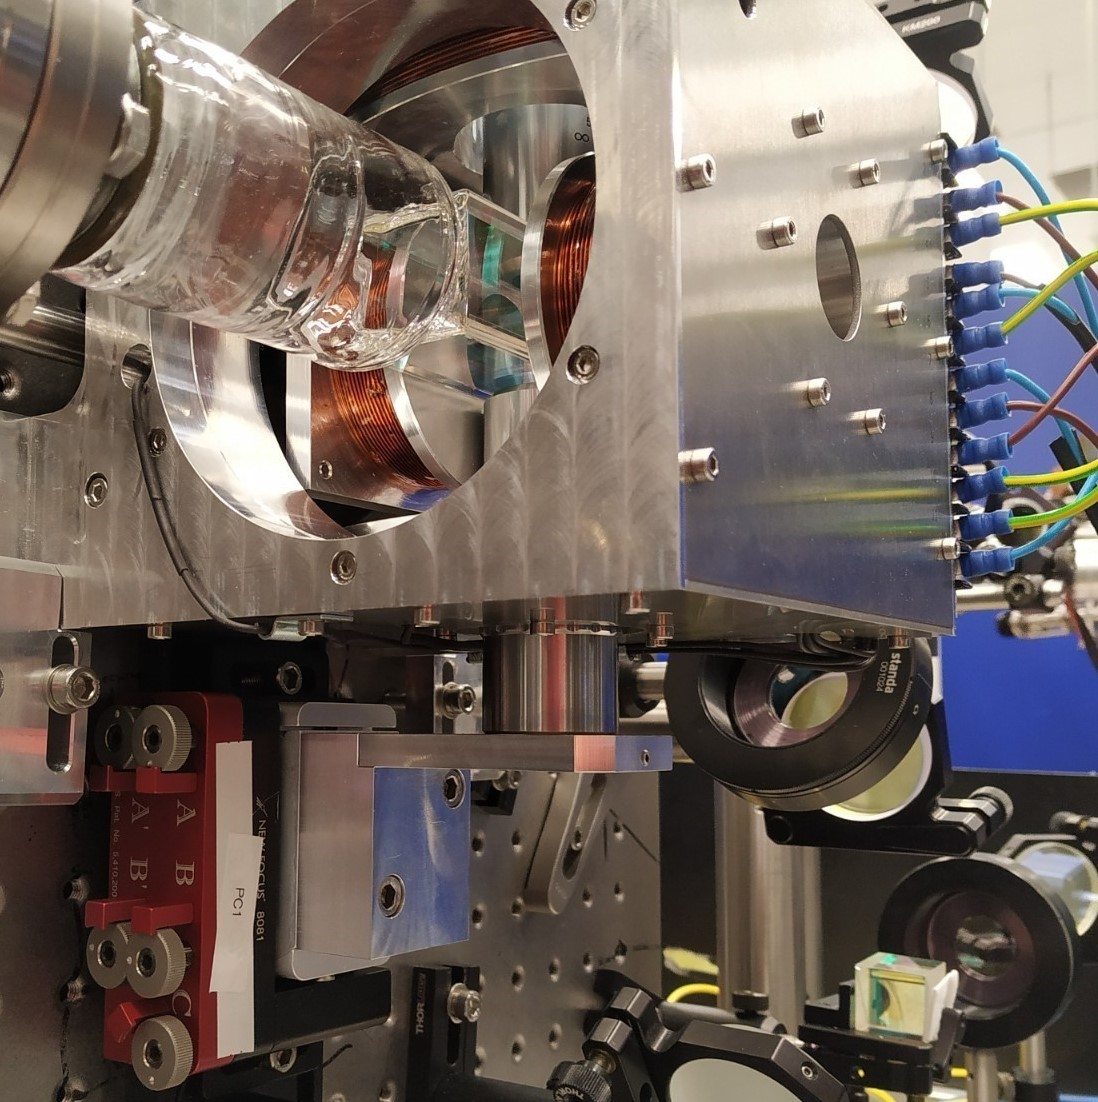
\includegraphics[height=7.6cm]{figures/CoilsCropped.jpg}
		\caption{}
		\label{fig:Coils1}
	\end{subfigure}
	\hfill
	\begin{subfigure}{.49\linewidth}
		\flushright
		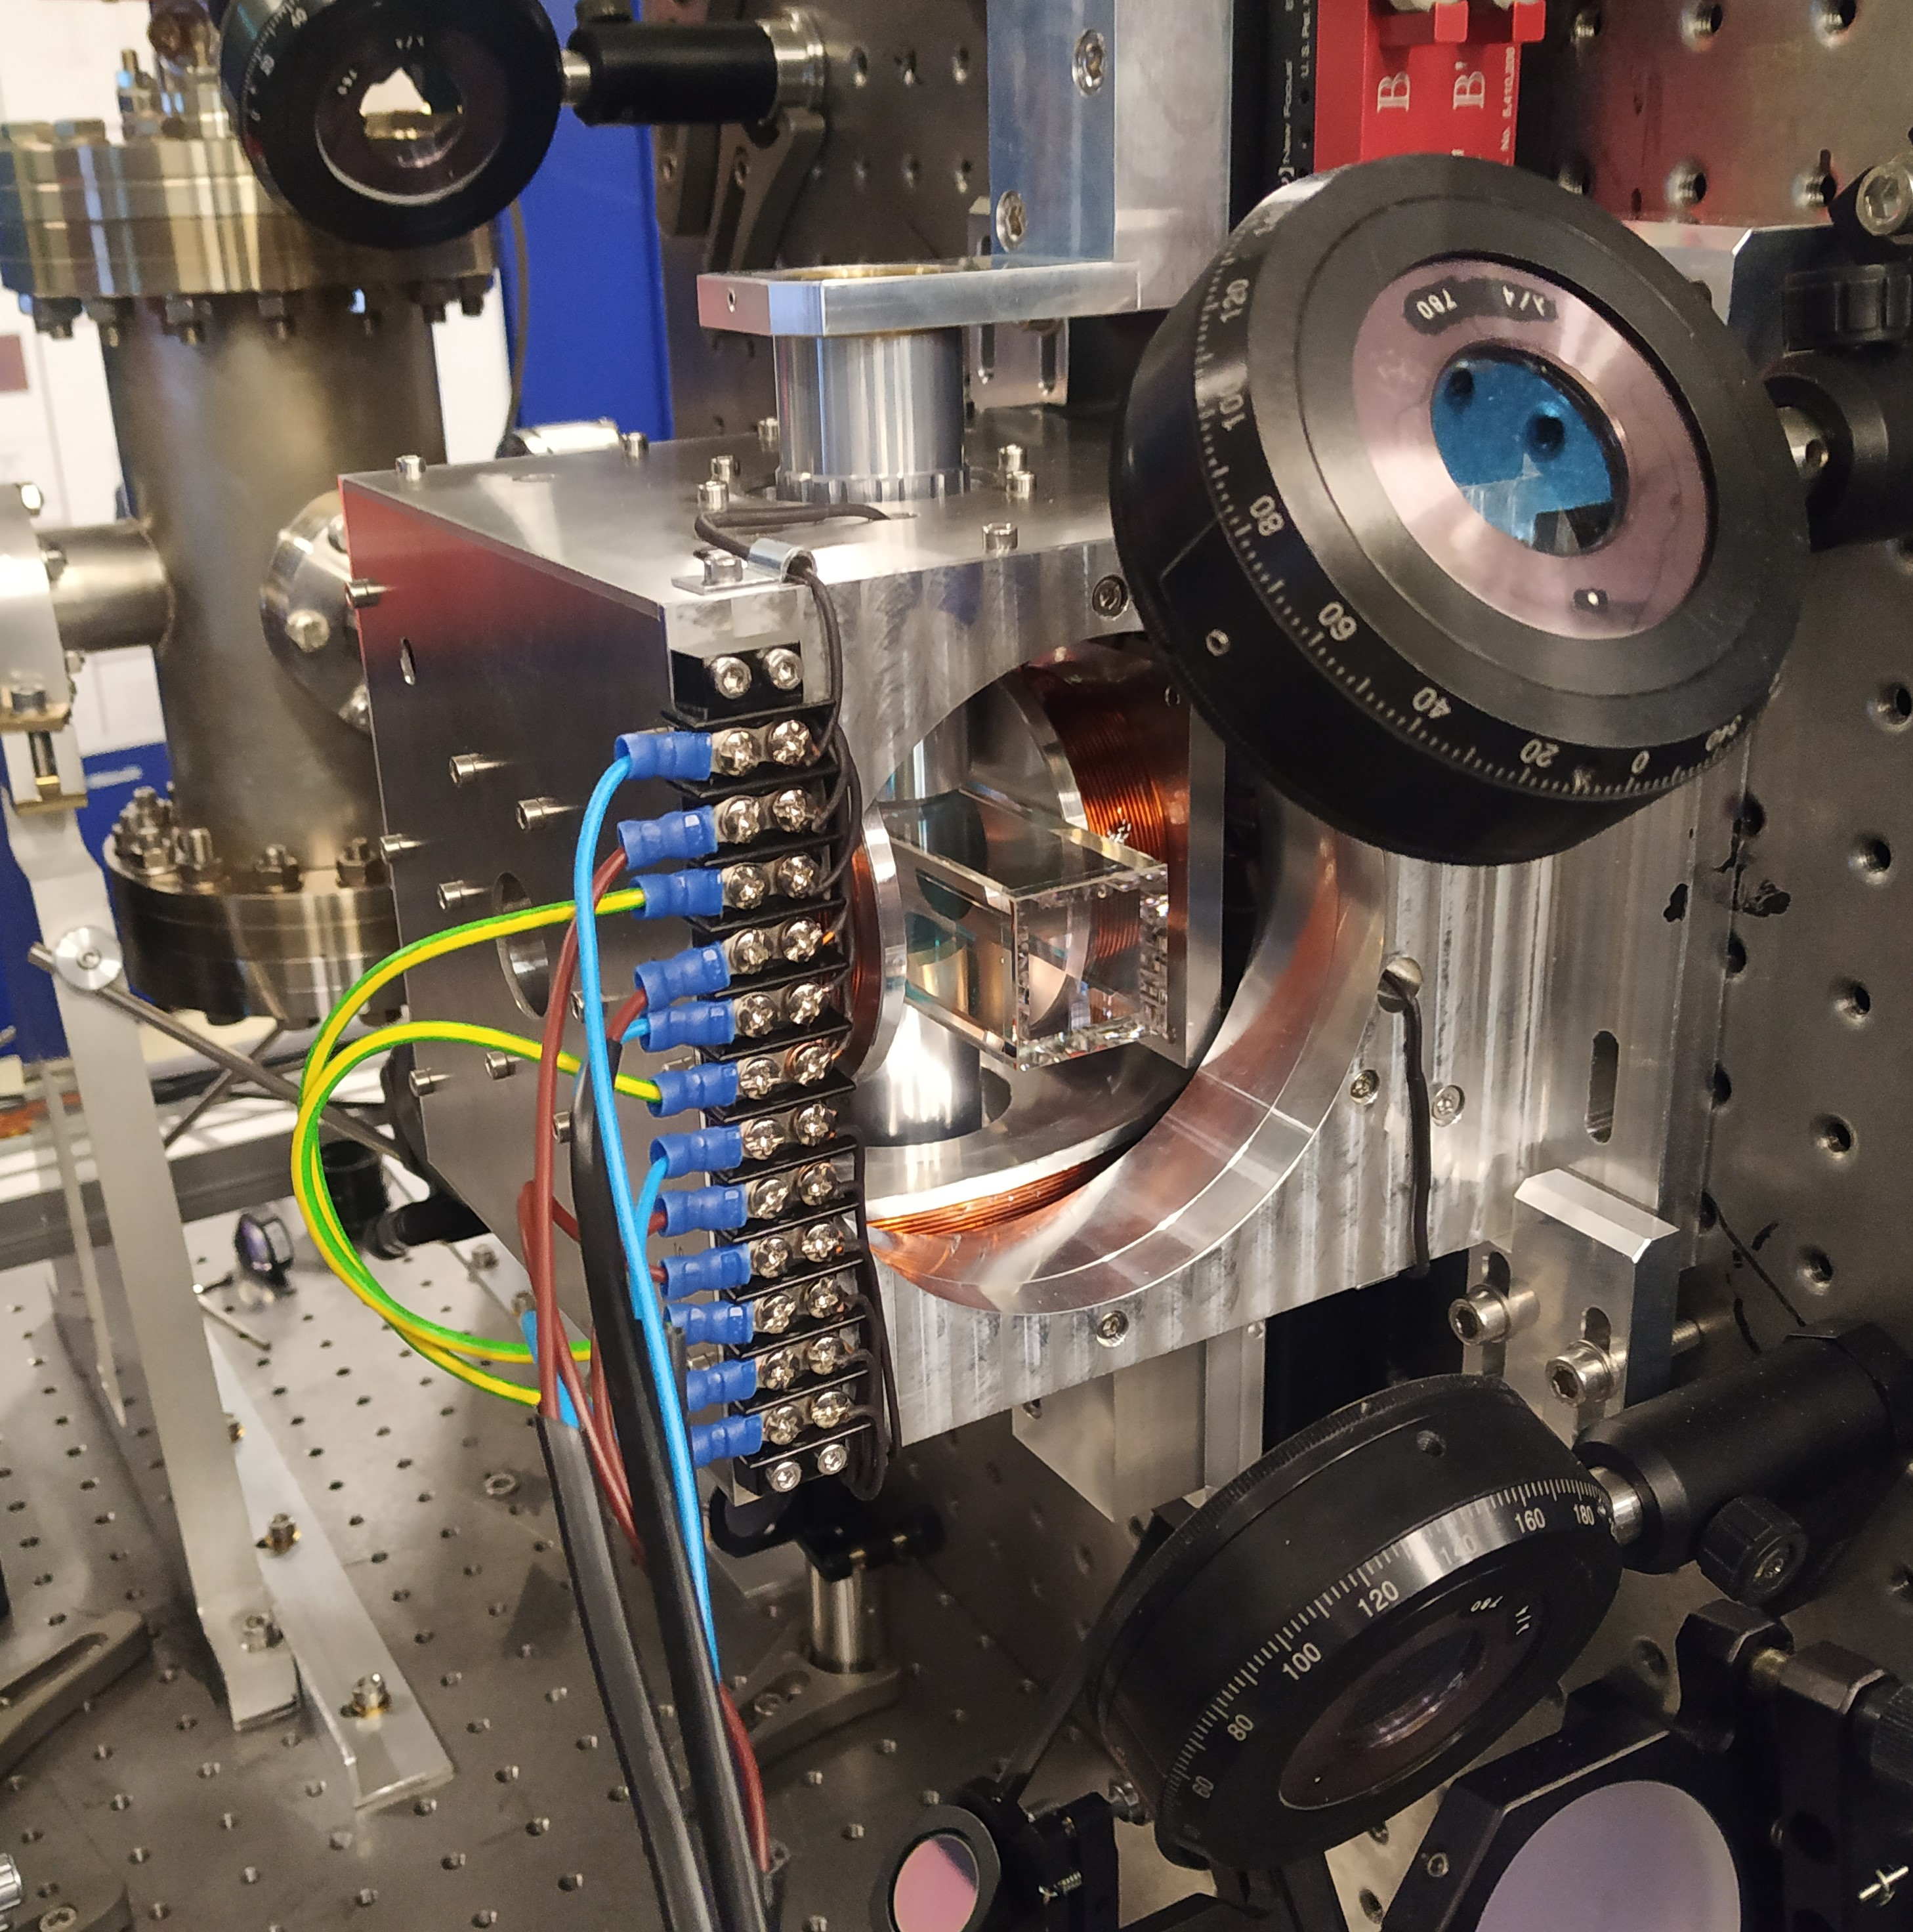
\includegraphics[height=7.6cm]{figures/CoilsCropped2.jpg}
		\caption{}
		\label{fig:Coils2}
	\end{subfigure}
	\caption{
	\textsf{\textbf{a)}} and  Housing for the magnetic field coils. 
	The glass cell slides into the magnetic field coils enclosure.
    The microscope objectives are positioned on 5-axis piezo controlled stages using a custom aluminum mount. 
    \textsf{\textbf{b)}} Different angled picture, showing the vacuum vessel in the background as well. 
    The large holes in the enclosure for the coils is for the angled MOT beams.
    }
    \label{fig:Coils}
\end{figure}


\subsection{Overlap with MOT}\label{subsec:Overlap}

To load the tweezers with ultra-cold atoms, it is to be overlapped with the magneto-optical trap.
The most straightforward method is to move the MOT in 3D-space using additional bias coils.
To this end, a magnetic field coil holder was designed by Deon Janse van Renseburg and Rik van Herk. 
It is shown in \cref{fig:Coils} and features a set of Anti-Helmholtz field coils producing a quadrupole magnetic as well as a set of coils in the directions perpendicular to it.
The coils perpendicular to the anti-Helmholtz coils are not exactly Helmholtz because of space limitations, more about this in the thesis of Rik van Herk \cite{Herk2022}.
We found moving the MOT to work very nicely over a range of $\sim 1$ cm, which is more than plenty in overlapping with the \ac{ODT}.
We did notice however, the MOT changing shape for larger bias fields. 
Probably, the magnetic field gradient is not fully linear.
This should pose no issue, however.

To ensure we are overlapped with the ODT, we bring the \ac{Ti:S} laser producing the tweezer pattern to the resonance frequency of \ac{Rb}.
This will make the tweezer visible on the top camera as it no longer blocked by the band-pass filter.
On this top camera, we can overlap the \ac{MOT} in the horizontal direction, and move the MOT vertically until we are in focus. 
Because the frequency is now resonant, and the scattering force becomes important, we can also verify we are destroying the MOT by off-balancing it, which we can see on the horizontal camera in \cref{fig:GlassCellSide}.
Using this method: one camera for 2D overlap and one camera for the vertical overlap, we verify we are overlapped in 3D space. 

The power supply used to drive the coils\footnote{KORAD KC3405 programmable DC power supply} as well as the \ac{AOM}s are controlled by a custom Python control program written by Deon Janse van Renseburg, with a graphical user interface in \textit{PyQt}.


\section{Imaging Tweezer Arrays}\label{sec:TweezerImaging}

As discussed in \cref{sec:ArraysResults}, we have two methods of seeing our tweezers.
Both methods should be possible with our current setup and we plan to use them both, combining the best of both worlds.
Contrary to the method in \cref{ch:tweezer}, information will be lost because the imaging resolution will be similar to the resolution limit of the tweezers. 

\subsection{Direct Imaging}

This is similar to the method in \cref{ch:tweezer}. 
But, because the glass cell has a outer thickness of 30 mm, we need an additional ultra-long working distance glass-thickness compensated objective.
The microscope objective has a working distance when imaging through 3.5 mm N-BK7 glass of 15.08 mm, but we know that the glass cell has 4 mm thick quartz glass.
As a result, the paraxial rays focus a distance $d(1-1/n)$ further, where $d$ is the excess thickness and $n$ the refractive index of NBK-7.
Marginal rays focus further, but are corrected for using the spherical aberration pattern. 
Thus, we estimate the working distance in conjunction with this glass is $15.18$ mm. 
Thus, it should be possible to get a second objective in focus, but this requires positioning the objective less than $0.2$ mm close to the glass cell.
The tweezer beam coming out of the second objective can be focused onto a linear CCD camera. 
The direct tweezer image can be used to verify the array remains aberration-free during the experiment. 
Additionally, it can be used to dynamically adapt the weight factors in the \ac{GSW} algorithm. 

We did not manage to get a parallel beam out of the top microscope objective: shown in \cref{fig:GlassCellSide} the objective forms a focus, which we use another achromatic lens for to correct. 
The objective is designed for parallel operation and will thus contain aberration. 
The working distance of the objective with 3.5 mm cover glass is 15.08 mm. 
Because of the extra glass with thickness $d_{ex} = 0.5/n$ mm, we estimate the new working distance to be $15.08 + d_{\text{ex}}(1-1/n) \approx 15.19$ mm.
This should be just enough to get both objectives in focus because the outer thickness of the glass cell is 30 mm, but even if the glass cell is almost touching we did not get a parallel beam. 
For now, it is not a problem the top camera is slightly abberated, but for the next iteration of the machine we ordered a new glass cell from Japan Cell with 25 mm outer thickness, so this should no longer be a problem anymore.  

\subsection{Fluorescence Imaging}

For actual useful cold-atom experiments, we want to see if we have actual atoms in the tweezer. 
The way to do this is to use atomic fluorescence.
If the atom in the tweezer sees near-resonant light, it can scatter light releases atomic fluorescence. 
Because this fluorescence is typically fairly weak, we should maximize the amount of scattered photons that we can actually collect. 
The fraction $\eta$ of fluorescence that can be captured by our imaging system is 

\begin{equation}\label{eq:Collection}
    \eta = \frac{\Omega}{4\pi} = 
    \frac{1}{2}\left(1-\sqrt{1-\frac{\text{NA}^2}{n^2}}\right)
\end{equation}
For $\textsf{NA}=0.5$ and $n=1$, this collection fraction is $\eta =0.067$. 
Because the amount of photons that can be collected from an atom in a tweezer is limited, it is important to maximize \cref{eq:Collection}.
We collect the laser-induced fluorescence using the same microscope objective as used for producing the tweezer, separating it from the tweezer beam using a \ac{DM} \footnote{Thorlabs DMLP805, 1 inch}.
This is shown in \cref{fig:GlassCellTop}.
This dichroic mirror has a 805 cut-off, which is why 820 nm was chosen for the dipole traps.
We could collect the fluorescence from the top objective as well, but this has the disadvantage that the top objective is looking directly in the dipole laser, which we found near impossible to fully separate from the relatively weak fluorescence signal. 

The fluorescence is steered onto the Andor Zyla 5.5 sCMOS camera chip covered by a 780 band-pass filter, see \cref{fig:GlassCellTop,fig:GlassCellSide}.
The pixel size is 6.5 $\mu$m, or 19.5 $\mu$m using $3\times3$ pixel binning. 
It is focused onto the chip using a $f= 55$ mm lens\footnote{Nikon Micro-NIKKOR 55 mm f/2.8}.
Using \cref{eq:InfinityMagnification} this comes down to a magnification factor of $13.75$.
Assuming our spots are $0.8$ $\mu$m in $1/e^2$ radius, which after convolution with the imaging optics is roughly $1.1$ $\mu$m.
With the $13.75$ magnification, it turns out $3\times 3$ binning is probably the best choice for us. 
Thus, the spots are imaged onto one $3\times3$ binned chip when aligned with the center of the spot.
By trying to map the tweezer spots one to one on the camera, the signal to noise ratio is maximized. 

We focus the sCMOS camera by adjusting the $f=55$ mm field lens.
We do not have a feature we can focus onto, but we know we should be focused at infinity to be in focus with our tweezer array. 
We ensure we focus at infinity by shining a laser source collimated by a fiber outcoupler directly onto our camera, adjusting the focus until the parallel is imaged onto the chip as a diffraction-limited spot. 


The near-resonant light we will refer to as the probe light. 
In principle, the MOT beams could be used for this, as they should be near-resonant as well. 
However, we were worried using the MOT beams would cause too much noise, as they have fairly high power we say quite a large amount of scattering in the vacuum chamber on the camera, especially from the angled beams, which can internally reflect in the glass cell.
To also control over the exact power, detuning as well as in which beam the probe light goes, we used a separate laser path for this. 
As shown in \cref{fig:RbLaserSetup}, we split off a tiny amount of power to a separate AOM, denoted as probe AOM. 
The probe is recombined with the MOT beams in \cref{fig:GlassCellTop}, but we have full control over which beam it will go because of the $\lambdaup/2$ plate.
We typically run the probe with a blue detuning of $\delta \sim +3\gamma$ (the transition is Stark shifted to the blue) and intensity $I = 0.5 I_{\text{sat}}$, which for our beam diameters comes down to $\sim0.$5 mW per beam. 

\subsubsection*{Experimental Sequence}

After letting the MOT build up for about 800 ms, we overlap the tweezer with it for about 150 ms.
This is done by a mechanical shutter, positioned on the \ac{Ti:S} laser table.
The delay of the shutter is in the order of a couple ms. 
During imaging, the MOT beams should be turned off, because its scattering will make the dipole traps impossible to see. 
The MOT beams can be shuttered off using the \ac{AOM}s in a matter of micro seconds. 
The MOT magnetic field will take longer to shut off due to Eddy currents in the coils. 
Rik van Herk measured a $1/e$ decay time of 8 ms, so we typically wait about 20 ms after turning off the MOT with the imaging. 
The imaging consists of triggering the probe beam as well as triggering the sCMOS camera at the same time. 
The triggering sequences are fed to the hardware using a programmable pattern generator custom built in our group. 
The imaging sequence is shown in \cref{fig:Sequence}.

\begin{figure}
    \centering
    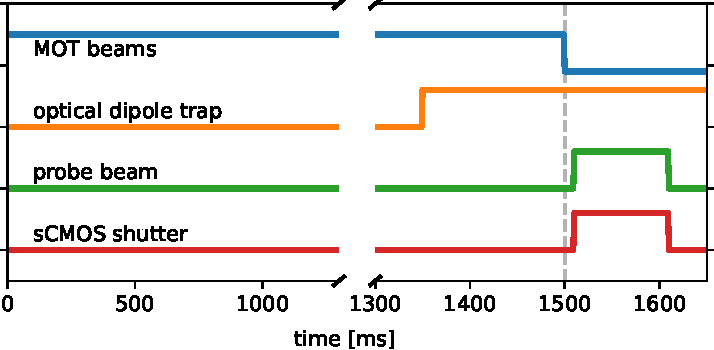
\includegraphics{figures/Sequence.pdf}
    \caption{Experimental sequence used to record laser-induced fluorescence from atoms trapped in an array of optical tweezers. }
    \label{fig:Sequence}
\end{figure}

For the atomic fluorescence pictures shown, the magnetic field was left on, but in the future it should be turned off. 
The reason is that the probe light is circularly polarized, which will cause Zeeman energy shifts in the array (\cref{eq:DetuningFull}).  
Due to Eddy currents, the magnetic field cannot be instantly switched off. 
Rik van measured measured a $1/e$ decay time of 8 ms when turning off the field \cite{Herk2022}, which in our case is definitely useable 


\subsubsection*{Images}

Below we show several images of atoms in our tweezer. 
These images were recorded using the aforementioned experimental sequence. 
We also performed exactly the same experimental sequence, but without turning no the dipole trap laser. 
The latter should only yield background as a result of atoms remaining from the expanding MOT or scattered photons from the probe beam. 
We subtracted the two images from each other, yielding the image in \cref{fig:fluorescence}


\begin{figure}
    \centering
	\begin{subfigure}{.49\linewidth}
		\centering
		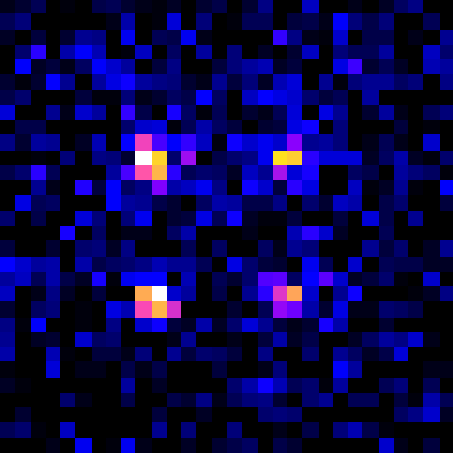
\includegraphics[height=5.5cm]{figures/2x2fluorescence.pdf}
		\caption{}
		\label{fig:fluor2x2}
	\end{subfigure}
	\hfill
	\begin{subfigure}{.49\linewidth}
		\centering
		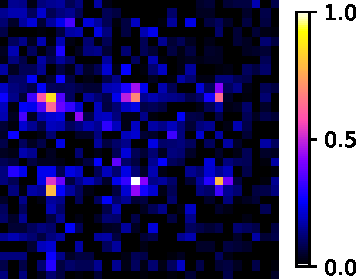
\includegraphics[height=5.5cm]{figures/2x3fluorescence.pdf}
		\caption{}
		\label{fig:fluor2x3}
	\end{subfigure}
	\caption{
	Fluorescence imaged onto the sCMOS camera when \textsf{\textbf{a)}} applying a $2\times2$ array pattern to the SLM and \textsf{\textbf{b)}} a $2\times 3$ array.
	Averaged over 50 runs.
    }
    \label{fig:fluorescence}
\end{figure}

This procedure was averaged a number of times as the signal to noise ratio was too low when not averaging. 
It is unclear why this is the case, most most likely it is not because too little atoms are loaded into the tweezer.
The reason is that our atom density of $\sim 10^9$ is comparable to the values mentioned in \cite{Schlosser2002} and are of similar order of magnitude to our collaborators at the University of Amsterdam.
Also, we have a relatively high atom temperature for loading optical tweezers, which should mean we have an even larger loading rate $R$ (\cref{eq:LoadingTweezer}).
This can be described by the following model \cite{Kuppens2000}

\begin{equation}
    R \propto n_0 \bar{v} A\propto n_0 T^{1/2} w_0^2.
\end{equation}

Here, $A$ is the area of the dipole trap as seen by the atom approaching with velocity $\bar{v}$. In our case $A \propto w_0^2$.
This model, which is only applicable in initial loading of the tweezer would thus predict that it is unlikely we have a loading rate that is too low. 

Rather, it is possible that the signal to noise ratio of the detection is too low. 
We also see that for more averages, the signal to noise significantly improves. 
Possible causes are that at the moment, we do not have a physical shutter in front of the camera. 
The camera should clear its array prior to beginning imaging, but we noticed that it does not do this. 
Also, the amount of photons we collect is quite small. Apart from the 0.069 collection fraction, 







\chapter{Conclusions and Outlook}\label{ch:conclusion}
    %conclusies

\section{Outlook}

\begin{itemize}
    \item single atom loading: fluorescence as a function of time
    \item Rydberg laser
    \item Subdoppler cooling scaling to more atoms
    \item 
\end{itemize}


\clearpage
\chapter*{Bibliography}
\addcontentsline{toc}{chapter}{Bibliography}%in inhoud

\printbibliography[heading=none]



%APPENDICES%

\begin{appendices}

 %appendix nummering sections, equations, figures5
\renewcommand{\thesection}{\thechapter.\arabic{section}}
\renewcommand\thefigure{\thechapter.\arabic{figure}}
\renewcommand\theequation{\thechapter.\arabic{equation}}
 
\setcounter{equation}{0}
\setcounter{figure}{0}

\chapter{Light-Matter Interaction: 2-level}\label{ch:LightMatter}

We follow \cite{Leeuwen2017}. For a 2-level atom (see \cref{fig:2LevelAtom}), the atomic Hamiltonian is best written down in its eigenstates, such that we have 

\begin{equation}\label{eq:AtomHamiltonian}
	\mathcal{H}_A = \hbar \omega_g \ket{g}\bra{g} + \hbar \omega_e \ket{e}\bra{e}.
\end{equation}
Where the eigenvalues are $\hbar \omega_g$ and $\hbar \omega_e$, and they satisfy the Schrodinger equation

\begin{subequations}\label{eq:AtomEigenStates}
	\begin{align}
		i \hbar \dot{\ket{g}}= \hbar \omega_g \ket{g}, \\
		i \hbar \dot{\ket{e}}= \hbar \omega_e \ket{e}.
	\end{align}
\end{subequations}
Where the dote denotes the temporal derivative. We treat the light field as a time-dependent perturbation $H_{I}(t)$ such that the total Hamiltonian is

\begin{equation}\label{eq:Perturbation}
	\mathcal{H} = \mathcal{H}_A + \mathcal{H}_{I}(t).
\end{equation}
The time evolution of \cref{eq:Perturbation} can be written down in the unperturbed states as

\begin{equation}\label{eq:TwoLevel}
	\ket{\psi} = c_g(t) e^{-i \omega_g t} \ket{g} + c_e(t) e^{-i \omega_e t} \ket{e}.
\end{equation}
Substituting \cref{eq:Perturbation,eq:TwoLevel} in the Schrodinger equation yields, after canceling the terms that involve \cref{eq:AtomEigenStates} 

\begin{equation}\label{eq:TwoLevelSchroedinger}
	i \hbar \left(\dot{c}_g(t) e^{-i \omega_e t}+\dot{c}_e(t) e^{-i \omega_e t} \right) = c_g(t) \mathcal{H_I}(t)\ket{g} e^{-i \omega_g t} + c_e(t) \mathcal{H_I}(t) \ket{e} e^{-i \omega_e t}.
\end{equation}
Because $\{\ket{g},\ket{e}\}$ constitute an orthogonal set, we can exploit a trick where we multiply \cref{eq:TwoLevelSchroedinger} from the left by $\{\bra{g},\bra{e}\}$, yielding a set of two coupled equations:

\begin{subequations}\label{eq:CoupledEq}
	\begin{align}
		i \hbar \dot{c}_g &= e^{-i \omega_0 t} 
		\left[c_g \bra{g} \mathcal{H}_I \ket{g} + c_e \bra{g} \mathcal{H}_I \ket{e}\right],  \\
		i \hbar \dot{c}_e &=  e^{ i \omega_0 t} 
		\left[c_g \bra{e} \mathcal{H}_I \ket{g} + c_e \bra{e} \mathcal{H}_I \ket{e}\right].
	\end{align}
\end{subequations}
Where the explicit time dependence of $c_g$ and $c_e$ will be omitted from now on. In order to calculate the matrix elements in \cref{eq:CoupledEq}, the Wigner-Eckart theorem can be used. If $\ket{g}$ and $\ket{e}$ are described by the quantum numbers $J$, $M$ and $\alpha$ (total and magnetic quantum number, and $\alpha$ keeps track of the other quantum numbers), the matrix elements can be evaluated as 

\begin{equation}\label{eq:WignerEckart}
	\bra{J_g M_g \alpha_g} \hat{T}_q^n \ket{J_e M_e \alpha_e} = 
	(-1)^{J_e-M_e} \begin{pmatrix}
		J_e & n & J_g \\
		-M_e& q & M_1
	\end{pmatrix}
	\bra{J_g\alpha_e } | \hat{T}^n | \ket{J_g\alpha_g}.
\end{equation}
Where $q \in \{-1,0,1\}$ is the spherical component index, the 2 x 3 matrix is the $3j$-symbol, which is in principle known and can be formulated in terms of  Glebsch-Gordan coefficients. $\hat{T}_q^n$ is a spherical tensor operator. The term $\bra{}|\hat{T}^n|\ket{}$ is the reduced matrix element \cite{Leeuwen2017}. Calculating the matrix elements will not be done here, but many $3j$-symbols will turn out to be zero. For example, the diagonal matrix elements will turn out to be zero, such that \cref{eq:CoupledEq} reduces to

\begin{subequations}\label{eq:NoOffDiagonal}
	\begin{align}
		i \hbar \dot{c}_g &= e^{-i \omega_0 t}  c_e \bra{g} \mathcal{H}_I \ket{e}, \\
		i \hbar \dot{c}_e &=  e^{ i \omega_0 t} c_g \bra{e} \mathcal{H}_I \ket{g}  .
	\end{align}
\end{subequations}
We will now calculate the matrix elements for the classical light field. Up until this point, the derivation was exact for the 2-level atom. Now we will make a series of approximations to get to a solvable set of equations \cite{Leeuwen2017}

\begin{equation}\label{eq:CosineLightField}
	\mathbf{E}(z,t) = \mathbf{E}_0 \cos{(k z - \omega t)}.
\end{equation}
Under the dipole approximation, the interaction Hamiltonian is \cite{Foot2005}

\begin{equation}
	\mathcal{H_I} = - e\mathbf{r}\cdot \mathbf{E}.
\end{equation}
Because an atom is orders of magnitude smaller than the wavelength of the radiation field, we can safely set $z=0$. The Hamiltonian simplifies to 

\begin{equation}\label{eq:OscillatingHamiltonian}
	\mathcal{H}_I = \frac{-e E_0 z}{2} \left(e^{i \omega t} + e^{-i \omega t}\right).
\end{equation}
Substitution of \cref{eq:OscillatingHamiltonian} in \cref{eq:NoOffDiagonal} yields

\begin{subequations}\label{eq:ClassicalHamSubstituted}
	\begin{align}
		i \hbar \dot{c}_g &= \frac{e E_0}{2} c_e[e^{ i (\omega-\omega_0) t}+e^{-i(\omega+ \omega_0)t}] \bra{g} z \ket{e}, \\
		i \hbar \dot{c}_e &= \frac{e E_0}{2} c_g[e^{+i (\omega+\omega_0) t}+e^{-i(\omega- \omega_0)t}] \bra{e} z \ket{g}.
	\end{align}
\end{subequations}
We assume $\omega \gg \delta$, such that $\omega+\omega_0 \approx 2\omega_0$ which oscillates much faster than the $\omega-\omega_0=\delta$ term. Over time scales of absorption and emission processes, this much faster contribution averages out. This is known as the \ac{RWA} \cite{Vredenbregt2020,Loudon2000} Thus we are left with

\begin{subequations}\label{eq:Rabi}
	\begin{align}
		i \hbar \dot{c}_g &= c_e \frac{\hbar \Omega  }{2} e^{ i \delta t},\\
		i \hbar \dot{c}_e &= c_g \frac{\hbar \Omega^*}{2} e^{-i \delta t}.
	\end{align}
\end{subequations}
Where the so-called Rabi frequency 

\begin{equation}\label{eq:RabiFrequency}
	\Omega \equiv \frac{e E_0}{\hbar} \bra{g}\mathbf{r}\ket{e},
\end{equation}
and its complex conjugate is introduced. In order to remove the time-dependence of \cref{eq:Rabi}, we can turn 'look' at them from a 'rotating frame'. More formally, it is a basis transformation described by the unitary matrix $\mathcal{U}$ \cite{Foot2005}

\begin{equation}\label{eq:RotatingFrame}
	\begin{pmatrix}
		\tilde{c}_g \\ 
		\tilde{c}_e
	\end{pmatrix} =
	\mathcal{U}
	\begin{pmatrix}
		c_g \\
		c_e
	\end{pmatrix} =
	\begin{pmatrix}
		e^{i \delta t/2} & 0\\
		0 & e^{-i \delta t/2}
	\end{pmatrix}
	\begin{pmatrix}
		c_g \\
		c_e
	\end{pmatrix} =
	\begin{pmatrix}
		c_g e^{i\delta t/2}\\
		c_e e^{-i \delta t/2}
	\end{pmatrix}.
\end{equation}
Substituting \cref{eq:RotatingFrame} in \cref{eq:Rabi} yields, after omitting the tiles, the matrix equation \cref{eq:MatrixEvolution}

\begin{equation}
	i \hbar \begin{pmatrix}
		\dot{c}_g \\ 
		\dot{c}e
	\end{pmatrix}
	= \frac{\hbar}{2} \begin{pmatrix}
		\delta & \Omega \\ \Omega^* & -\delta 
	\end{pmatrix} 
	\begin{pmatrix}
		c_g \\ c_e
	\end{pmatrix}.
\end{equation}



%\chapter{Fourier Optics}



% %\section{Fourier Optics}

% For describing the optics in this project, we need a description of diffraction. Ray optics will not suffice for this, wave optics is needed. One elegant description is Fourier optics. 

% We start with a result from Maxwell's equations in an electromagnetic medium in three dimensions, where $\mathbf{u(\mathbf{r},t)}$ can denote either the electric or magnetic field vector.

% \begin{equation}\label{WaveEquation}
% 	\nabla^2 \mathbf{u}(\mathbf{r},t) = \frac{n^2}{c^2} \frac{\partial^2 \mathbf{u}(\mathbf{r},t)}{\partial t^2}
% \end{equation}

% For monochromatic light, which is true to good approximation for a laser, we can substitute the ansatz $\mathbf{u(\mathbf{r},t)} = Re\{ \mathbf{U}(\mathbf{r}) e^{i \omega t} \}$, yielding the time-independent so called Helmholtz equation:

% \begin{equation}\label{Helmholtz}
% 	(\nabla^2 + k^2)  \mathbf{U}(\mathbf{r}) = 0
% \end{equation}

% \section{Huygens-Fresnel Principle}

% The Huygens-Fresnel principle can be expressed mathematically as \cite{Goodman2005}:

% \begin{equation}\label{eq:HuygensFresnel}
% 	U(P_0) = \frac{1}{i \lambda} \iint U(P_1) \frac{e^{i k r}}{r} \cos{\theta} \text{d}x' \text{d}y'
% \end{equation}

% Because $\cos{\theta} = z/r$, we can write \ref{eq:HuygensFresnel} as:

% \begin{equation}\label{eq:HuygensFresnel2}
% 	U(x,y) = \frac{z}{i \lambda} \iint U(x',y') \frac{e^{i k r}}{r^2} \text{d}x' \text{d}y',
% \end{equation}

% where $r$ is given by $\sqrt{(z^2 + (x-x')^2 +(y-y')^2)}$. Because the square root is difficult to work with, $r$ can be approximated by assuming $z^2 \gg (x-x')^2 + (y-y')^2$, which is really the same thing as assuming the angle $\theta$ is small (paraxial approximation). We can then expand the definition for $r$ to first order as

% \begin{equation}\label{eq:FirstOrderR}
% 	r = z \sqrt{1+ \Big(\frac{x-x'}{z}\Big)^2 + \Big( \frac{y-y'}{z}\Big)} \approx z \left[ 1 + \frac{1}{2} \Big(\frac{x-x'}{z}\Big)^2 + \frac{1}{2} \Big( \frac{y-y'}{z} \Big)^2\right]
% \end{equation}

% When $r$ appears in the denominator, we can approximate the term in square brackets as unity. For terms appearing in the exponent however, we cannot do this. Substituting \cref{eq:FirstOrderR} in \cref{eq:HuygensFresnel2}:

% \begin{equation}\label{eq:HuygensFresnel3}
% 	U(x,y) = \frac{e^{i k z}}{i \lambda z}\iint U(x',y') \exp{\frac{i k}{2 z} \left[(x-x')^2+(y-y')^2\right]} \text{d}x' \text{d}y'
% \end{equation}

% \subsection{Fraunhofer Approximation}

% the term in square brackets in \cref{eq:HuygensFresnel3}, when expanded yields:

% \begin{equation}
% 	(x^2+y^2) + (x'x+y'y)+(x'^2+y'^2)
% \end{equation}

% As a final approximation, if the Fraunhofer approximation is met: $2z \gg k \max{(x'^2+y'^2)}$, $x'x+y'y \gg x'^2+y'^2$ and we can drop the latter two terms in the integration. If the constant phase term involving $x^2+y^2$ is brought in front of the integral we are left with the Fraunhofer diffraction integral:

% \begin{equation}\label{FraunhoferDiffractionIntegral}
% 	U(x,y) = \frac{e^{i k z}}{i \lambda z} e^{i(x^2+y^2)/(2z)} \iint U(x',y') e^{\frac{-i 2 \pi}{\lambda z} (x'x+y'y)}\text{d}x' \text{d}y'
% \end{equation}

% In \cref{FraunhoferDiffractionIntegral}, the 2D Fourier transform property can be recognized, for frequencies $f_x=x/(\lambda z)$ and $f_y=y/(\lambda z)$:

% \begin{equation}
% 	U(x,y)=\frac{e^{i k z}}{i \lambda z} e^{i(x^2+y^2)/(2z)} \mathscr{F}\{ U(x',y')\} 
% 	\Bigr\rvert_{f_x=x'/\lambda z,f_y=y'/\lambda z}
% \end{equation}

% where $\mathscr{F}\{\}$ denotes the 2D Fourier transform, evaluated at frequencies $f_x=x'/\lambda z$ and $f_y=y'/\lambda z$, more conveniently written as $\mathscr{F}\{U\}(f_x,f_y$) from now \cite{Bijnen2015}.

% \subsection{Transfer Function Lens}

% The SLM produces an intensity pattern in the far field. To project this pattern a distance smaller than infinity away, a positive lens is used. To describe the optics of the SLM pattern, this lens should thus be taken into account. In Fourier optics, the effect of a thin lens can be described as

% \begin{equation}\label{lensTransfer}
% 	U'_{lens}(x,y) = t(x,y) U_{lens}(x,y),
% \end{equation}

% where t(x,y) is the so-called transfer function of a lens. The derivation for paraxial approximation is done from p. 97 in \cite{Goodman2005} and \cite{Dijk2012} and will not be repeated here. The result for a thin lens is:

% \begin{equation}\label{transferFunction}
% 	t(x,y)=\exp{\left[\frac{-i k}{2 f}(x^2 + y^2)\right]}
% \end{equation}

% **insert some more stuff** In the end, one finds the following relation between the SLM plane and the focal plane of the Fourier lens:

% \begin{equation}\label{relationSLMlens}
% 	U(x, y)=\frac{e^{i \frac{k}{2 f}\left(1-\frac{d}{f}\right)\left(x^{2}+y^{2}\right)}}{i \lambda f} \iint U_{\text{SLM}}(x', y') e^{-i \frac{2 \pi}{\lambda f}(x'x+y'y)} \mathrm{d}x'\mathrm{d}y'
% \end{equation}

% However, the quantity typically measured is power or intensity, which is the absolute value squared of the complex amplitude \cite{Dijk2012,Bijnen2015}

% \begin{equation}\label{FourierFinal}
% 	I(x,y) = |U(x,y)|^2 \propto \left| \mathscr{F} \{ PU_0 e^{i \Phi(x',y')} \} (\frac{x'}{\lambda f},\frac{y'}{\lambda f})\right|^2
% \end{equation}

% Where $U_0$ notes the input intensity complex amplitude, $P$ the aperture function of the SLM and the phase factor $e^{i \Phi(x,y)}$ the phase modulation of the SLM. In practice, we have a finite amount of pixels available on the SLM and $\Phi(x',y')$ is not continuous, therefore we use the discrete Fourier transform (DFT) which uses a more efficient algorithm also known as the fast Fourier transform (FFT). 




%\chapter{Light matter interaction}


% Because light is the main tool used in the field of ultracold atoms to manipulate atoms, here a brief description of light-matter interaction will be discussed. The matter has been discussed more thoroughly in several sources \cite{Metcalf1999,Vredenbregt2020,Leeuwen2017}.
% \section{Light Matter Interaction}



%\chapter{Strehl Ratio}

% In practice, there will always be some wavefront-distortion present as a result of aberrations. This distortion can be measured using a Shack-Hartmann wavefront sensor. A quicker method is using the definition of the Strehl ratio, a measure of the intensity contained in the central lobe of the Airy disk compared to the theoretical diffraction-limited maximum \cite{Sortais2007}. The definition of the Strehl $S$ ratio in terms of the RMS wavefront error $\Delta$ is 

% \begin{equation}\label{Strehl}
% 	S = 1- 4\pi^2\frac{\Delta^2}{\lambdaup^2}
% \end{equation}

% A commonly used criterion is $S>0.8$ for the system to be diffraction-limited. This sets a limit on the RMS wavefront error of $\Delta < 0.071 \lambdaup$.


 
\end{appendices}


\end{document}
